


% Couverture
\MakeUGthesePDG

\clearpage
\ifodd\value{page}\hbox{}\newpage\fi

\begin{center}\textbf{\large Étude et amélioration de l'exploitation des architectures NUMA à travers des supports exécutifs}

\quad

\textbf{Résumé}
\end{center}

L'évolution du calcul haute performance est aujourd'hui dirigée par les besoins des applications de simulation numérique.
Les secteurs comme l'aéronautique, les applications militaires, la météorologie, ou encore le nucléaire ont besoin de simuler des phénomènes à grande échelle, se traduisant parfois par la résolution de systèmes de systèmes linéaires à plusieurs millions d'inconnues.

Toutes ces simulations sont au final exécutées sur des supercalculateurs qui peuvent proposer plusieurs milliers de coeurs, et qui sont découpés en un très grand nombre de noeuds de calcul ayant eux un nombre de coeurs beaucoup plus faible.

Si l'évolution des processeurs du siècle dernier était caractérisée par une augmentation de la fréquence, de nos jours l'évolution des processeurs est caractérisée par une multiplication du nombre de coeurs.
Dans ces architectures à mémoire partagée moderne, la mémoire est découpée en plusieurs blocs physiques différents, avec chacun leur propre contrôleur.
La conséquence direct de ce découpage est que le temps d'accès à la mémoire est devenu non-uniforme : il dépend directement de quel processeur essaye d'accéder à quelle partie de la mémoire.
On appelle ce genre d'architectures NUMA (pour \emph{Non Uniform Memory Access}) et elles sont aujourd'hui la brique de base pour créer des supercalculateurs.

L'exploitation efficace des machines NUMA est critique pour l'amélioration globale des performances des supercalculateurs.

Cette thèse est axée sur l'amélioration des standards et techniques pour l'exploitation des machines NUMA, et peut se découper en deux parties : une partie a été dédié à fournir au programmeur les moyens de comprendre et analyser, et mieux spécifier le comportement des parties critiques de son application, et l'autre partie se concentre sur différentes améliorations du programme chargé d'exécuter les applications : le support exécutif.



\quad

\textbf{Mots-clés} : trucs

\begin{center}\textbf{\large TODO }

\quad

\textbf{Abstract}
\end{center}

TODO

\quad

\textbf{Keywords} : stuff

%\begin{savequote}[8cm]
%<< Une thèse sans théorème ce n'est pas une thèse >>
%\qauthor{Denis Trystram}
%\end{savequote}
%% Remerciements...
%\chapter*{Remerciements}

%\begin{todo}
%Test todo
%\end{todo}


% TOC
\cleardoublepage
\dominitoc
\makeatletter
\renewcommand{\tableofcontents}[1][\contentsname]{%
  \chapter*{#1}
  \@starttoc{toc}
}
\makeatother
\tableofcontents

%TODO : Ajouter papiers Christiane Pousa Ribeiro à la biblio

\begin{savequote}[6cm]
<< Elle sert à quoi ta thèse ?  >>

\end{savequote}
\chapter{Introduction}
\chaptertoc

L'évolution du calcul haute performance est aujourd'hui dirigée par les besoins des applications de simulation numérique.
Ces applications sont omniprésentes dans l'industrie, et concernent parfois même directement le grand public.

Par exemple des secteurs comme l'aéronautique, les applications militaires, ou encore le nucléaire ont besoin de simuler des phénomènes à grande échelle, se traduisant parfois par la résolution de systèmes linéaires à plusieurs millions d'inconnues.
Les prévisions météorologiques à destination du grand public sont faites à l'aide d'applications simulant les interactions entre les différents éléments de l'atmosphère.
Il en va de même pour tout ce qui se rapporte à l'étude de la propagation des ondes sismiques dans le sol, ou de la prévision de l'impact d'un séisme sur un bassin de population.

Toutes ces simulations sont au final exécutées sur des supercalculateurs, et il n'y a pas de limite au nombre de ressources qu'elles peuvent utiliser : que ce soit pour améliorer la précision de la simulation, ou augmenter la taille de l'ensemble simulé, elles pourront toujours bénéficier d'un plus grand nombre de ressources.
Avoir plus de ressources peut également permettre d'exécuter un plus grand nombre de simulations simultanément, voire de les coupler entre elles.

Si les supercalculateurs peuvent proposer plusieurs milliers de cœurs, ils sont en fait composés d'un grand nombre de nœuds de calcul avec un nombre de cœurs beaucoup plus faible.
Ces machines peuvent proposer, en plus de processeurs traditionnels, des accélérateurs plus ou moins spécifiques comme des GPUs ou des FPGA, formant une architecture dite \emph{hétérogène}.
La très grande majorité des nœuds de calcul intègrent plusieurs processeurs qui accèdent à une mémoire commune.

Contrairement aux processeurs du siècle dernier pour lesquels un changement de génération s'accompagnait d'une augmentation de leur fréquence de fonctionnement, l'évolution des processeurs contemporains se traduit aujourd'hui par la multiplication du nombres de cœurs de calcul qu'ils embarquent.
Pour illustrer ce phénomène il suffit de regarder par exemple la gamme de produits proposés par Intel : la première génération de Pentium 4 - Willamette - lancée par Intel en 2000 était constituée d'un unique cœur cadencé à 1.5GHz. 6 ans plus tard, la dernière génération de Pentium 4 - Cedar Mill - était également consituée d'un seul cœur, mais cette fois cadencé à 3.6 GHz. 10 ans plus tard en 2016, les processeurs de la génération Skylake d'Intel i7 ne dépassent pas les 3.4GHz de fréquence, mais tous ont 4 cœurs physiques au lieu d'un seul.

Avec ce changement de design, les modalités d'accès à la mémoire ont été repensées pour éviter les goulots d'étranglement se formant lors des accès concurrents de plusieurs cœurs au même bus mémoire. Le moyen qui a été trouvé pour éviter trop de contention sur le bus mémoire fut de diviser la mémoire en plusieurs blocs physiques différents, avec chacun leur contrôleur.
La conséquence directe de ce changement est que le temps d'accès à la mémoire est devenu non uniforme : il dépend directement de quel processeur essaye d'accéder à quelle partie de la mémoire.
On appelle ce genre d'architectures NUMA (pour \emph{Non Uniform Memory Access}) et elles sont aujourd'hui la brique de base pour créer des supercalculateurs.

L'amélioration des performances générales d'un supercalculateur passe donc directement par l'optimisation de l'exploitation des machines NUMA.
Plusieurs techniques de programmation permettent de cibler ce genre d'architectures.
On peut notamment citer des techniques statiques à base de boucles parallèles.
En pratique cela marche particulièrement bien pour les applications où toutes les itérations des boucles sont régulières et où leur temps d'exécution est prévisible.
Néanmoins il existe beaucoup de situations où ce n'est pas le cas.
Un exemple typique est celui des applications de parcours de graphes, qui sont généralement irrégulières.
Mais même dans le cas d'une application où le travail peut sembler régulier, comme par exemple une multiplication de matrices, l'ajout d'une variabilité dans le temps des accès mémoires rend le temps d'exécution difficile à prévoir, et peut entrainer un déséquilibre de charge.


Les techniques d'ordonnancement dynamiques peuvent garantir une utilisation plus efficace des ressources.
L'une des plus communes est l'ordonnancement par vol de travail : l'application est exprimée comme un graphe de flot de données, chaque sous-partie - tâche - consommant et produisant des données.
Un programme dédié - le support exécutif - a la charge d'exécuter ce graphe : à chaque fois qu'un processeur devient inactif, il va récupérer une tâche disponible pour l'exécuter.
Pour que cela soit efficace, il faut pouvoir exprimer un maximum de parallélisme : plus il y a de parallélisme, mieux on est capable d'équilibrer la charge au cours de l'exécution.

Les modèles de programmation standards ont su s'adapter : par exemple OpenMP, qui est le standard \emph{de-facto} pour ce genre d'architectures, ne proposait au départ que du parallélisme de boucles. Les dernières versions proposent de la programmation par tâche avec dépendances de données.
En revanche ces modèles de programmation présentent toujours un manque lorsqu'il s'agit d'exploiter efficacement les machines NUMA.
Le programmeur doit donc faire de gros efforts pour effectuer des optimisations spécifiques peu portables, par exemple via des bibliothèques externes pour contrôler précisément le placement des données.
Les outils standards et non intrusifs permettent simplement de distribuer les pages de la mémoire sur les différentes parties physiques : cela a pour avantage d'améliorer l'uniformité des temps d'accès à la mémoire, mais pas d'améliorer le temps d'accès moyen, rendant donc les processeurs uniformément mauvais vis à vis de l'accès à la mémoire.

Cette thèse est axée sur l'amélioration des standards et techniques pour l'exploitation des machines NUMA, et cela passe par plusieurs étapes : tout d'abord fournir au programmeur les moyens de comprendre et analyser le comportement des parties critiques de son application.
Ensuite lui permettre de fournir plus d'information au support exécutif, principalement en lui permettant d'exprimer une \emph{affinité} entre ses tâches et les ressources de la machine.
Et enfin proposer des techniques d'ordonnancement prenant en compte ces informations, dans le but d'améliorer efficacement les performances globales de l'application.





\section{Objectifs}\label{sec:intro:objectives}

L'objectif principal de cette thèse était d'étudier les améliorations possibles de l'exploitation des architectures NUMA, à l'aide d'un modèle de programmation à base de tâches.
Cela a été découpé en trois axes de travail.


\subsection*{Analyse du comportement d'applications sur machine NUMA}

Avant de pouvoir penser aux améliorations, il faut commencer par analyser les différents points améliorables, tant du côté logiciel que matériel.
Si l'on souhaitait cibler les modèles de programmation à base de tâches, il fallait néanmoins choisir l'un des modèles existants pour l'étude concrète, et ce choix s'est porté sur OpenMP.

Face à l'absence de suite de benchmarks ciblant certaines fonctionnalités d'OpenMP que nous souhaitions utiliser, nous avons commencé par publier une suite de benchmarks, les KASTORS~\cite{Virouleau2014}.
Les applications présentes dans cette suite ont été adaptées depuis des applications existantes, afin d'utiliser les constructions dont nous avions besoin, et qui sont aujourd'hui utilisées par la communauté.

Nous avons également écrit un outil plus générique, \outil, afin de pouvoir évaluer plus précisément certaines parties ciblées des applications.
L'objectif derrière cet outil est de se libérer de certaines contraintes se présentant lors de l'observation de ces parties de code au cours de l'exécution complète du programme.
En extrayant les parties critiques on peut faire varier à loisir, et précisément, des paramètres tels que le placement des données ou le jeu de données en entrée, afin d'analyser finement quels impacts ils ont et comment l'architecture sous-jacente réagit.


\subsection*{Quelles améliorations pour l'utilisateur et le support exécutif ?}

À partir des conclusions tirées du point précédent, le second objectif était de trouver, proposer, et évaluer des améliorations possibles, tant pour l'utilisateur que pour le support exécutif.

Ces réflexions ont donné lieu à deux contributions : la première est axée sur la réponse au besoin de l'utilisateur, en proposant une clause |affinity| pour les tâches OpenMP~\cite{Virouleau2016b}.
Cette clause a pour but de permettre à l'utilisateur d'indiquer explicitement un lien fort entre une tâche et une ressource de la machine, que ce soit un coeur, un noeud, ou une donnée.
La seconde est axée sur l'extension du support exécutif~\cite{Virouleau2016a}, d'une part pour faciliter la distribution des données sur la machine, et d'autre part pour exploiter les informations disponibles sur les données manipulées par les tâches, dans le but d'améliorer la localité des données au cours de l'exécution.


\subsection*{Place des travaux dans l'évolution du matériel et du logiciel}

Au cours de cette thèse les architectures NUMA ont évolué, on peut alors se demander dans quelle mesure l'évolution du matériel impacte les travaux de cette thèse.
Le dernier objectif est donc d'analyser les travaux effectués - voir les compléter - afin de proposer des approches indépendantes du matériel, dans le but de faciliter le travail du programmeur et du développeur de support exécutif à l'avenir.

Parmi nos travaux, \outil propose une approche transposable à tout type d'architecture, et nous avons fait des travaux préliminaires sur un simulateur, qui à partir des données de cet outil peut donner un aperçu des performances de l'application complète.
Le coût - en temps - de changer l'implémentation utilisée par un support exécutif est assez important, ces travaux préliminaires ont pour objectif de donner un premier aperçu de l'impact que pourrait avoir une modification de l'ordonnancement par le support exécutif.
Cela permet ainsi, lors du "portage" d'une application ou d'un support exécutif sur une nouvelle architecture, d'estimer son comportement, et évaluer si des changements dans l'un des deux sont nécessaires.

\section{Plan}\label{sec:intro:outline}

TODO



\part{Problématiques impliquées et approches existantes}

\begin{savequote}[6cm]
<< Some great quote  >>
\qauthor{François Broquedis}
\end{savequote}
\chapter{Contexte}\label{chap:contexte}
\chaptertoc

\pagebreak

L'objectif de ce chapitre est de donner au lecteur les connaissances de base nécessaires pour l'appréciation du reste de la thèse.
Elles peuvent se classer en trois catégories~: la première concerne les architectures cibles pour nos travaux. Il y a une grande variété de matériels disponibles pour le calcul haute performance : la section~\ref{sec:context:numa} décrit en détails les architectures à mémoire partagée actuelles (NUMA), et la section~\ref{sec:context:os} décrit leur gestion par le système d'exploitation.
La seconde concerne les modèles de programmation à base de tâche. La section~\ref{sec:context:others} décrit les techniques modernes utilisées pour cibler les architectures NUMA, et décrit en détails les concepts de base ainsi que les points clés pertinents à nos travaux. La section~\ref{sec:context:openmp} est dédiée à OpenMP, modèle de programmation qui a été utilisé pour l'application des travaux de la thèse.
Enfin la section~\ref{sec:context:runtimes} regroupe des informations générales concernant le rôle des supports exécutifs dans l'exécution d'applications parallèles à base de tâches.

\section{Architectures à mémoire partagée}\label{sec:context:numa}


Les architectures à mémoire partagée ont subit des changements majeurs liés à l'évolution des processeurs.
L'augmentation du nombre de cœurs par processeur a introduit des problèmes d'accès à la mémoire centrale : dans une architecture composée d'une unique mémoire, plusieurs cœurs cherchant à accéder à la mémoire vont rentrer en concurrence et introduire de la contention et donc des délais dans l'accès à la mémoire, ce qui pénalise formtement les performances.

Pour pallier ce problème, les constructeurs ont divisé la mémoire centrale en plusieurs parties physiquement distinctes, appelées \emph{nœuds}.
Le nœud NUMA est le composant de base pour une architecture NUMA.
Chaque nœud est constitué d'une partie de la mémoire centrale, d'un contrôleur local d'accès à ce bloc mémoire, ainsi que d'un certain nombre de cœurs de calcul.
L'ensemble des nœuds de la machine sont ensuite reliés entre eux par un réseau d'interconnexion.
La topologie de l'interconnexion ne permet généralement pas d'avoir des nœuds équidistants, ce qui introduit une hiérarchie mémoire.

Malgré le fait que les différentes parties de l'architecture soient physiquement séparées, le système d'exploitation voit l'ensemble comme une unique machine.

Nous décrivons dans un premier temps les caractéristiques techniques communes d'un processeur multicœur d'un nœud dans les sections~\ref{sec:context:numa:cache}, et~\ref{sec:context:numa:node}, puis celles des systèmes d'interconnexion des nœuds dans la section~\ref{sec:context:numa:interconnect}.
Elles ont une influence directe sur le comportement du nœud au sein de la machine.

\subsection{Caches des processeurs}\label{sec:context:numa:cache}

Le cache est une mémoire pour laquelle le temps d'accès est bien meilleur que pour la mémoire centrale, mais dont la capacité est beaucoup plus restreinte. Il peut être spécifique à un cœur du processeur, ou partagé par plusieurs d'entre eux.

\subsubsection{Fonctionnement}

Au niveau des accès le fonctionnement d'un cache est légèrement différent de celui de la mémoire centrale : plutôt que de lire uniquement un octet, c'est généralement une partie fixe de la mémoire contenant cet octet qui est chargée.
On appelle cette quantité une \emph{ligne de cache}, et un exemple de taille standard pour une ligne de cache est 64 octets (8 nombres réels double précision).

Lorsqu'une instruction demande le chargement d'une valeur située en mémoire, le contrôleur du cache reçoit la requête du processeur, détermine la ligne de cache correspondante à partir de l'adresse demandée, et effectue l'une des deux opérations suivantes :
\begin{description}
  \item [Cache hit :] si la ligne correspondante est déjà présente dans le cache la donnée est directement retournée au cœur.
  \item [Cache miss :] si la ligne n'est pas présente le contrôleur de cache va charger la valeur depuis la mémoire centrale vers le cache, et retourner la valeur au cœur.
\end{description}

%(je vire ça vu qu'on ne parle de niveaux de cache que plus tard) Si le cœur a accès à plusieurs niveaux de cache, la requête est transférée au niveau supérieur, et seul le dernier niveau effectue la requête à la mémoire centrale.
Une fois qu'une ligne est chargée dans le cache, elle n'y reste pas de manière permanente, plusieurs raisons décrites ci-après peuvent entraîner son \emph{éviction} du cache :

\begin{itemize}
  \item Le maintien de la cohérence : lorsqu'un cœur modifie une ligne de cache dans son propre cache, cette même ligne est \emph{invalidée} dans les caches des autres processeurs qui en disposent d'une version.
Si un processeur essaie de faire un accès sur une ligne invalidée, elle sera rechargée depuis la mémoire centrale, générant un \emph{cache miss}.
  \item Le dépassement de la capacité du cache : il est assez commun que l'ensemble des données manipulées par le programme ne tienne pas dans le cache.
Lorsqu'une requête est effectuée sur une ligne, qu'elle n'est pas présente dans le cache, et que le cache est plein, le contrôleur choisira une ligne à évincer du cache pour faire de la place à la nouvelle ligne.
Le choix de la ligne à évincer est un sujet très étudié, et le prochain paragraphe revient sur les politiques d'éviction communément utilisées.
  \item Le conflit d'adresse : dans certains modèle de caches, certaines lignes correspondant à des adresses mémoires doivent être stockées dans le même emplacement du cache.
    Si elles sont requises alternativement pendant l'exécution du programme, elles se sortiront mutuellement du cache.
    Ce problème dépend directement de l'\emph{associativité} du cache, qui est traitée dans le paragraphe suivant.
\end{itemize}



\subsubsection{Associativité}

Le cache ne pouvant être suffisamment grand pour contenir toute la mémoire, il faut pouvoir déterminer l'association entre l'adresse d'une ligne dans la mémoire centrale et son emplacement dans le cache.
Il y a trois grandes catégories d'associativité utilisées par les caches :
\begin{itemize}
  \item Les caches à association directe (\emph{direct-mapped cache}) : dans ce système, chaque ligne de la mémoire est associée à exactement un emplacement dans le cache.
    Ce système est simple, propose le meilleur temps de réponse, mais est peu prévisible et à taille identique est moins efficace que les deux autres catégories.
  \item Les caches complètement associatifs (\emph{fully associative cache}) : dans ce système, chaque ligne de la mémoire peut être associée à n'importe quel emplacement dans le cache.
    Cela permet de maximiser l'utilisation de l'espace disponible, mais cela induit un coût supplémentaire pour déterminer l'association entre une ligne et son emplacement.
  \item Les caches N-associatifs (\emph{N-way associative cache}) : ce système est un compromis entre les deux précédents.
    Chaque ligne de la mémoire peut être associée à exactement N emplacements dans le cache.
    Cela implique un certain nombre d'opérations sur les adresses des lignes, et l'espace pris par le composant ainsi que le temps d'accès moyen dépend directement de la valeur de N.
\end{itemize}

Hill et al.~\cite{Hill1989} (Table III) illustre l'impact de l'associativité sur la proportion de cache miss et catégorise son origine (conflit d'adresse, défaut de capacité du cache, chargement normal de la donnée).
Cela permet de dégager deux observations : d'une part qu'augmenter l'associativité permet de diminuer les cache miss.
D'autre part que les défauts de cache ayant une forte associativité sont quasi exclusivement dus à la capacité du cache, alors que pour les caches à association directe les conflits d'adresse sont une part non négligeable des cache miss.

\subsubsection{Niveaux de caches}

Il y a en général 3 niveaux de cache dans ces architectures :
\begin{itemize}
  \item L1 : C'est le cache le plus "proche" du CPU, mais aussi le plus petit - typiquement quelques Ko. Il est généralement découpé en deux parties distinctes : une partie pour les instructions, une autre pour les données.
  \item L2 : Ce cache est physiquement plus éloigné du processeur et présente une latence d'accès plus importante que le L1, mais propose une plus grande capacité de mémoire. Il a un ordre de grandeur de quelques centaines de Ko.
  \item L3 : Ce cache est généralement le cache de dernier niveau - \emph{Last Layer Cache (LLC)} - sur un processeur. La latence pour y accéder est plus importante que le L2, mais sa capacité est bien supérieure, pouvant en général atteindre plusieurs Mo.
\end{itemize}

En fonction des fabricants, ces caches peuvent être soit \emph{inclusifs} (c'est-à-dire que toutes les données présentes dans le L1 sont également présentes dans le L2), ou \emph{exclusifs} (c'est-à-dire qu'une donnée est garantie de n'être présente que dans l'un des caches).

Au sein d'un nœud, le L3 est généralement partagé par tous les cœurs, alors que les caches L1 et L2 sont spécifiques à un cœur.

\begin{figure}[ht]
  \centering
  \includegraphics{processor_small}
  \caption{Schéma d'un processeur multicœurs}\label{fig:context:schema-caches}
\end{figure}

La figure~\ref{fig:context:schema-caches} décrit la hiérarchie typique d'un processeur multicœurs que l'on peut trouver sur un nœud NUMA.
Dans cet exemple, le processeur dispose de 8 cœurs, et chaque cœur dispose d'une cache L1 indépendant pour les données et les instructions (32 Ko chacun), d'un cache L2 (256 Ko), et d'un cache L3 partagé avec 7 autres cœurs (20 Mo).


En général les développeurs d'applications pour le HPC accordent beaucoup d'attention à l'optimisation de leur application, pour que les parties de code séquentiel critiques utilisent des données qui puissent être contenues dans le L1/L2.
De même, beaucoup d'optimisations au sein des compilateurs visent également cet objectif.

Lorsqu'il s'agit de cibler des architectures NUMA, on va tout particulièrement s'intéresser au L3, qui représente la mémoire la plus rapide accessible par tous les cœurs d'un même nœud.

\begin{todo}
TODO : ref + paragraph sur les caches configurables du ryzen.
Pas trouvé de ref sur le ryzen parlant de cache configurable, mais j'ai trouvé Jenga : http://people.csail.mit.edu/sanchez/papers/2017.jenga.isca.pdf
\end{todo}

\begin{table}[ht]
\def\arraystretch{1.5}
\centering
\begin{tabular}{|c||c|c|c|c|}\hline
  Cache & \multicolumn{2}{c|}{Intel Sandy Bridge} & \multicolumn{2}{c|}{Intel Broadwell}  \\ \cline{2-5} 
 & Latence & Bande passante & Latence & Bande passante \\ \hline
 L1 & 1.6 ns & 16 Go/s & 1.8 ns & 32 Go/s \\ \hline
 L2 & 5.0 ns & 14 Go/s & 5.4 ns & 17 Go/s \\ \hline
 L3 & ~20 ns & 8 Go/s & ~24 ns & 9 Go/s \\ \hline
 RAM & ~90 ns & 4 Go/s & ~140 ns & 7 Go/s \\ \hline
\end{tabular}
\caption{Tableau synthétiques des latences et bande passante en fonction du niveau de cache et du processeur}\label{tab:synthese-processeurs}
\end{table}

Afin de donner un ordre d'idée des latences et bande passantes sur les différents processeurs, le tableau~\ref{tab:synthese-processeurs} récapitule les chiffres en fonction de la génération du processeurs.
Les mesures ont été faites à l'aide de l'outil LMbench~\cite{McVoy1996}. Pour la latence, les temps considérés sont ceux du benchmark |lat_mem_rd| avec un accès aléatoire à la mémoire.
Pour la bande passante les temps considérés sont ceux du benchmark |bw_mem|, en utilisant un équivalent de |memcpy|.
Pour la latence, tout effet potentiel du prefetcher est annulé par l'utilisation de \emph{pointer chasing} (l'adresse de la case suivante à charger est située dans la case courante), ce qui n'est pas le cas pour la bande passante.

Comme on peut le voir sur ces chiffres, le coût d'accès à la mémoire principale est prohibitif par comparaison aux différents caches, y compris le L3.
Les différentes caractéristiques de ces processeurs et des machines sur lesquels ils sont intégrés seront étudiées en détails dans la section~\ref{sec:contribs:machines}.

\subsubsection{Politiques d'éviction}

Le choix de la ligne de cache à remplacer lorsque le cache est plein a un impact direct sur les performances, et les politiques de remplacement ont été très étudiées par les différents acteurs de la communauté académique et industrielle.

La politique optimale serait de remplacer la ligne qui sera réutilisée le plus tard, mais ce genre de clairvoyance est impossible à implémenter en pratique.
Un certain nombre d'alternatives ont donc été imaginées, et sont décrites ci-après :
\begin{itemize}
  \item Random : cette politique choisi une ligne à remplacer au hasard. Sa simplicité la rend simple à implémenter en pratique, et a notamment été utilisée dans les processeurs ARM Cortex-R~\cite{ARM-Cortex-R}.
  \item First-In First-Out : comme son nom l'indique, la ligne remplacée est la première qui est rentrée dans le cache parmi celles présentes.
  \item Least Recently Used (LRU) : dans cette politique, chaque ligne dispose de plusieurs bits représentant la date de la dernière utilisation de cette ligne. La ligne remplacée est celle ayant été utilisée il y a le plus longtemps.
  \item Pseudo-LRU : cette politique offre une version dégradée permettant de gérer des caches de grandes tailles.
Lorsque l'associativité du cache dépasse un certain seuil, le coût d'implémentation de LRU devient trop important~\cite{Kedzierski2010}, l'alternative proposée par les politiques pseudo-LRU est donc de remplacer une ligne parmi celles utilisées il y a le plus longtemps.
Cela permet de limiter le nombre de bits nécessaire pour tracer les lignes à remplacer potentielles.
  \item Autres politiques adaptatives : dans le cas spécifique du cache de dernier niveau (LLC), certains fabriquants comme Intel utilisent des politiques adaptatives présentées comme supérieures à Pseudo-LRU, prenant en compte la fréquence à laquelle sont utilisées certaines lignes de caches.
    \emph{Dynamic Re-Referency Interval Prediction} en est un exemple, qui a été présenté parmi d'autres par Jaleel et al.~\cite{Jaleel2010}.
\end{itemize}

La politique pseudo-LRU semble être la plus utilisée par les fabricants de processeurs tous niveaux de cache confondus. Al-Zoubi et al.~\cite{Al-Zoubi2004} proposent une évaluation complète et détaillée de l'impact des politiques d'éviction en fonction de l'associativité du cache, justifiant le choix des constructeurs.



\subsection{Autres caractéristiques matérielles des processeurs}\label{sec:context:numa:node}

En plus des caches qui nous intéresseront tout particulièrement dans la suite de ce manuscrit, les processeurs ont également d'autres composants matériels dont il est important d'avoir conscience, mais qui ont une place plus limitée dans le contexte de cette thèse : il s'agit des instructions vectorielles et de l'hyperthreading, décrit ci-après.

\subsubsection{Instructions vectorielles}\label{sec:context:numa:simd}

Le concept de vectorisation est l'action d'appliquer une même instruction sur plusieurs données (ou un \emph{vecteur} de données) nécessitant la même opération.
Ce type d'instructions est appelée SIMD, pour \emph{Single Instruction Multiple Data}.

Afin d'illustrer ce point, il suffit d'imaginer que l'on souhaite additionner deux vecteurs d'entiers :
\begin{lstlisting}
int vecteur_a[8] = { 1 };
int vecteur_b[8] = { 1 };
int addition[8];
for (int i = 0; i < 8; i++) {
  addition[i] = vecteur_a[i] + vecteur_b[i];
}
\end{lstlisting}

Exécuter la boucle complète effectuerait 8 additions sur des entiers.
En supposant que la largeur des registres (et des instructions) du processeur est de 64 bits, et que la taille d'un |int| est 32 bits, on "gaspillerait" en fait 32 bits par addition.

Étant donné que l'on souhaite effectuer la même opération (une addition), sur des éléments indépendants du tableau, on peut alors aisément grouper deux additions successives dans la même instruction : il suffit de mettre un entier de 32 bits sur la partie haute du registre, et un deuxième entier sur la partie basse, d'effectuer l'instruction, et de faire l'opération inverse pour stocker le résultat dans le tableau.
De plus la vectorisation permet au processeur d'optimiser la décomposition de l'instruction en micro opérations et donc l'utilisation du pipeline.
Au final on divise le nombre d'itérations, mais aussi le nombre d'accès mémoire et d'opérations par 2.


\begin{todo}
  j'ai pas trouvé la ref des procs vectoriels sur ACM, (re)demander à Thierry
\end{todo}

Des extensions au jeu d'instructions x86 ont été créées afin de pouvoir opérer sur des éléments plus larges que 64 bits, et la plupart des architectures des processeurs récents utilisent des registres plus larges que le type le plus large en C (|long long|, 64 bits).
La première d'entre elles, SSE (\emph{Streaming SIMD Extensions}), a été introduite par Intel dès 1999 et a évolué régulièrement, agrandissant progressivement la taille des registres jusqu'à l'extension AVX-512, permettant d'effectuer des instructions sur des registres de 512 bits.

La plupart des processeurs actuels (depuis les Sandy Bridge d'Intel, et les Bulldozer d'AMD, en 2011) supportent au moins l'extension AVX avec des registres de 128 bits.

\subsubsection{Hyperthreading}

Chaque cœur possède un certain nombre d'UAL (Unité Arithmétique et Logique) qui lui sont privées. Lorsqu'il est en attente d'une donnée de la mémoire centrale, ces UALs ne sont pas utilisées, et des cycles CPU sont donc "perdus" à ne rien faire.

Afin de maximiser l'utilisation de ces ressources, certains processeurs Intel sont équipés de la technologie \emph{hyperthreading}.
Le concept est assez simple : avoir deux cœurs logiques (\emph{hyperthreads}) associés à un seul cœur physique.
De cette manière lorsqu'un thread est en attente sur une donnée (par exemple lors d'un chargement d'une donnée depuis la mémoire), le second peut profiter des UALs disponibles.

Pour des tâches peu gourmandes en ressources ou utilisant beaucoup de données, cela peut effectivement se traduire par un gain de performances, mais pour le cas des applications HPC il faut regarder le type d'applications utilisées pour savoir si on peut espérer un gain ou non.
En particulier les caches L1 et L2 sont partagés par les deux hyperthreads, donc si le code séquentiel généré est optimisé pour les tailles de caches correspondant, exécuter le même type de code séquentiel sur deux hyperthreads peut entrainer du \emph{cache trashing}.
Au meilleur des cas l'hyperthreading améliorera les performances mais ne sera pas forcément très efficace, atteignant par exemple entre 2.3 et 3.3 de speed-up pour 4 hyperthreads par cœur~\cite{Jeffers2016} sur les derniers processeurs d'Intel, les Xeon Phi.
Si l'application est très intensive en calcul et utilise au maximum les UALs, l'hyperthreading n'apportera pas grand chose, voire rien.

L'hyperthreading est généralement une option que l'on peut désactiver dans le BIOS de la machine, ou éviter en plaçant correctement les threads de son application.


\subsection{Interconnexion des nœuds}\label{sec:context:numa:interconnect}

L'une des parties majeures d'une machine NUMA est le système d'interconnexion entre les différents nœuds.
C'est cette partie qui va déterminer à quel point cela va être couteux d'accéder à la mémoire située sur un nœud distant, et donc à quel point l'aspect NUMA de la machine va impacter les performances d'une application.
Dans la majorité des cas, ce système d'interconnexion est \emph{cache-coherent}, c'est à dire que la cohérence de cache est assurée entre les différents nœuds par le matériel, et n'est pas la responsabilité du programmeur ou du support exécutif.
L'impact sur les performances peut être lié à la fois au protocole de cohérence de caches utilisé, ainsi qu'à la topologie de l'interconnexion des nœuds.


\subsubsection{Protocoles de cohérence de cache}

Le nombre de caches utilisés dans une machine NUMA peut être important, et la même ligne de la mémoire peut être présente dans plusieurs caches en même temps.
Il est important que l'état des différentes copies soit cohérent : par exemple si une ligne a été écrite et modifiée, les copies de cette ligne dans les autres caches doivent être mises à jour.

La plupart des protocoles se basent sur un ensemble d'états possibles pour une ligne de cache :

\begin{description}
  \item [Modified (M) :] la ligne a été modifiée dans le cache. Les données dans cette ligne ne sont donc pas cohérentes avec la mémoire principale. Quand la ligne est évincée, elle doit être écrite dans la mémoire principale.
  \item [Shared (S) :] la ligne est <<propre>> (non modifiée), elle existe dans d'autres caches mais est en lecture seule dans le cache courant. Cette ligne peut être évincée sans autre action.
  \item [Invalid (I) :] la ligne est soit absente du cache courant ou a été invalidé par un autre cache. Elle doit être récupérée depuis la mémoire principale (ou un autre cache qui en possède une copie valide).
\end{description}

Cet ensemble d'états de base forme le protocole \emph{MSI}, qui a ensuite été étendu avec plusieurs autres états :

\begin{description}
  \item [Exclusive (E) :] la ligne est présente uniquement dans le cache courant et elle est <<propre>>.
  \item [Owned (O) :] la ligne est présente dans plusieurs caches dans un état valide, mais seul le cache courant peut y effectuer des modifications.
    Cet état permet de partager des lignes qui ont été modifiées sans passer par une ré-écriture dans la mémoire centrale : le cache qui possède la ligne est responsable de fournir une version à jour, et d'écrire la ligne dans la mémoire centrale lorsque que la ligne est évincée.
  \item [Forward (F) :] cet état est similaire à l'état \emph{Shared}, mais indique au cache courant qu'il est responsable de satisfaire une requête en lecture sur la ligne.
\end{description}

Intel Quick Path Interconnect~\cite{Ziakas2010} (QPI) est le système d'interconnexion utilisé dans les machines d'expérimentation que nous avons utilisé, et qui sont décrites dans la section~\ref{sec:contribs:machines}.
Il implémente le protocole MESIF. Du à l'introduction de l'état \emph{F}, ce protocole est avantageux lorsque la latence de cache à cache est bien plus faible que la latence d'accès à la mémoire principale.

Pour implémenter ce protocole, il existe deux types de mécanismes :

\begin{itemize}
  \item À base de Snooping : chaque cache observe le trafic sur le bus mémoire pour des requêtes qui concerneraient les lignes de caches dont ils possèdent une copie. Un composant dédié peut effectuer un premier filtre pour restreindre le trafic lié au mécanisme de snooping. Néanmoins ce type de mécanismes ne passent pas bien à l'échelle, et aurait du mal à obtenir de bonne performance dans les architectures NUMA, où le nombre de caches est important.

  \item À base de répertoires : la donnée est placée dans un répertoire qui maintien la cohérence entre les caches. Chaque cache ne peut pas accéder directement à la mémoire principale mais doit passer par le répertoire.
\end{itemize}

Le QPI utilise un mix des deux mécanismes : il utilise des \emph{home agents} - comparables à des répertoires - qui sont les principales autorités pour fournir une version du cache depuis la mémoire principale.
Il utilise ensuite du \emph{snooping} pour satisfaire les requêtes des différents \emph{caching agents} (les entités qui possèdent un cache, telles que les processeurs).

Le QPI peut fonctionner avec deux modes de \emph{snooping} :
\begin{description}
  \item [Source snooping :] le \emph{caching agent} envoie la requête à tout le système. Les autres \emph{caching agent} peuvent répondre à la requête s'ils possèdent une version de la ligne de cache dans un état compatible. Le \emph{home agent} responsable de la ligne mémoire doit fournir une copie propre de la ligne de cache si besoin, et résoudre les conflits s'ils apparaissent.
  \item [Home snooping :] le \emph{caching agent} envoie la requête au \emph{home agent}, qui envoie ensuite une requête aux \emph{caching agents} qui possèdent une copie de la ligne et peut commencer à charger la ligne depuis la mémoire. L'un des \emph{caching agents} possédant la ligne et/ou le \emph{home agent} peut ensuite envoyer la réponse.
\end{description}

Le mode \emph{source snooping} a une latence plus faible que le mode \emph{home snooping}, mais passe moins bien à l'échelle.
C'est donc ce dernier qui est le plus adapté à un environnement NUMA, puisqu'il limite le nombre de requêtes envoyés sur le bus mémoire, et économise donc de la bande passante.


\subsubsection{Topologies}
\begin{todo}
  décrire le facteur NUMA et inclure des chiffre (reprendre graphe 2.1.2 plus bas)
\end{todo}

La topologie du système d'interconnexion peut être très différente d'une machine à une autre, et de multiples exemples existent dans les machines commercialisées.
Il existe des topologies plates, où chaque nœud est directement connecté aux autres (TODO: ref graph 2.1.2), des topologies où des couples de nœuds sont groupés entre eux et peuvent passer par un ou deux niveaux d'interconnexion (TODO: ref graph idchire).

Le nombre de rebonds - \emph{hops} - à effectuer avant d'accéder à la mémoire demandée impacte directement la latence et la bande passante, comme le montre le tableau comparatif de la figure~(TODO).

Chiffres :
même noeud: 2.11 GB/s
noeud meme group: 1.50 GB/s
groupe proche: 1.28 GB/s
groupe loin: 1.06 GB/s

GRAPHE : 2.1.2 les chiffres de base !
GRAPHE : 2.1.2 heatmap
GRAPHE : 2.1.2 montrer une version schématique d'une machine NUMA (2 socket, 1 socket/2 nœuds, idchire, knl)



\subsection*{Conclusion}

Cette partie s'est concentrée sur les connaissances de base nécessaires pour comprendre l'interaction entre les différents composants des architectures NUMA.
Le développeur d'application ne va généralement pas influer directement sur ces composants, en revanche il est capital d'avoir conscience des caractéristiques de chacun d'entre eux pour pouvoir expliquer facilement tel ou tel comportement de l'application.

Le premier composant logiciel qui va s'intéresser à la gestion directe du matériel est le système d'exploitation.
La section suivante revient sur les points relatifs à la gestion des architectures NUMA dans le système d'exploitation.

\section{Exploitation des architectures NUMA par le système d'exploitation}\label{sec:context:os}

Le support des machines NUMA dans Linux est arrivé dès 2003~\cite{Dobson2003}.
Détailler les dispositifs spécifiques à l'exploitation des machines NUMA au niveau système ne peut pas se faire sans avoir connaissance de certains mécanismes déjà existant.
La section suivante détaille donc la manière dont Linux gère la mémoire d'une machine <<standard>>, puis nous détaillerons les spécificités liées au caractère NUMA de la machine, ainsi que certaines bibliothèques externes utiles pour les programmeurs.

\subsection{Gestion de la mémoire}

La compréhension de la gestion de l'allocation de la mémoire par le système d'exploitation est un point critique lorsque l'on traite les machines NUMA.
Le système d'exploitation gère la mémoire par petit fragments, appelés \emph{pages}.
Lors de l'allocation d'un tableau par exemple, si sa taille dépasse celle d'une \emph{page}, l'espace mémoire alloué consistera donc de plusieurs pages.


Par défaut, lorsque l'allocateur mémoire demande au système la réservation d'un espace mémoire constitué de plusieurs \emph{pages} (lors d'un appel à |malloc| par exemple), le système retarde l'allocation effective de ces pages jusqu'au moment du premier accès - \emph{first-touch}.
C'est ce premier accès qui va déterminer l'allocation physique de la page : elle sera alloué sur le nœud local du processeur effectuant le \emph{first-touch}.

L'allocateur par défaut de la libc fait de la réutilisation de pages. Cela veut dire qu'après plusieurs allocations/libérations successives d'espace mémoire, vous n'obtenez pas forcément des nouvelles pages.
L'objectif derrière cela est de réduire le coût général d'une allocation, puisque l'allocation et la libération physique de nouvelles pages est couteux, et que réutiliser des pages supprime ce coût.
En revanche le corollaire de ce constat est que le contrôle de l'allocation physique par \emph{first-touch} n'est possible que lors de la première allocation des pages.
Ce problème est limité à la durée de vie du programme, s'il est susceptible d'apparaître, il est alors possible d'utiliser des librairies externes pour l'allocation de données, comme décrit dans la section suivante.

Enfin, un dernier détail mérite de l'attention, il s'agit de la taille des pages manipulées par le système.
En effet celle ci est configurable, et deux options sont généralement possibles : soit des pages de 4 Kilo octets, soit des - \emph{huge} - pages de 2 Mega octets.
L'impact de cette taille peut être important dans le cas d'un bloc de données s'étendant sur plusieurs pages : plusieurs requêtes de pages de petites tailles seront plus sensibles à la \emph{latence} de la mémoire, alors qu'une requête d'une page de grande taille équivalente sera plus sensible à la \emph{bande passante}.

\subsection{Prise en compte des architectures NUMA et bibliothèques externes}\label{sec:context:os:lib}

Avec l'arrivée du support des machines NUMA dans le système d'exploitation, plusieurs fonctionnalités fondamentales sont apparues et parmi elles on retrouve : la capacité d'obtenir des informations à propos de la machine, telles que le numéro de nœud d'un cœur donné, ou le numéro de nœud d'une adresse mémoire donnée.
On trouve aussi la possibilité de contrôler le placement d'un thread sur un ensemble de cœurs physiques à l'aide d'un masque d'affinité, ce qui permet par exemple de garantir la proximité physique de deux threads vis à vis d'un nœud, ou tout simplement de garantir qu'un thread sera exécuté par un cœur précis.

Plusieurs outils se sont basés sur ces briques de base pour proposer des fonctionnalités plus avancées, parmi eux \emph{numactl} et \emph{hwloc} :

\begin{description}
  \item [numactl~\cite{numactl} :] cet outil s'utilise avant l'utilisation d'un exécutable sur la ligne de commande. Il permet : de contrôler l'ensemble des cœurs (ou nœuds) sur lesquels les threads peuvent être placés au cours de l'exécution du programme ;
    de contrôler l'ensemble des nœuds NUMA sur lesquels peuvent être allouées des données ;
    et encore de modifier la politique d'allocation des pages du système, en permettant par exemple de distribuer les pages successives allouées, de manière cyclique sur un ensemble de nœuds.
  \item [hwloc~\cite{Broquedis2010} :] cet outil permet, entre autres, d'obtenir des informations précises sur le matériel et la topologie de la machine. Il expose les facteurs NUMA théoriques fournies par le matériel, et permet de visualiser les différents nœuds et groupes de nœuds.
  Il propose également des fonctions d'allocations plus fiable que |malloc|, garantissant l'allocation de nouvelles pages, et proposant différentes politiques d'allocations (incluant le \emph{first-touch}).
\end{description}


\bigskip

Dans la section précédente nous avons vu les détails concernant le matériel utilisé au cours de cette thèse, et dans cette section nous avons vu comment l'exploiter au niveau du système d'exploitation.

Le développeur d'application scientifique n'est généralement pas un spécialiste des fonctionnalités de base du système d'exploitation : il va plutôt être un expert de son application et des parties critiques qui la composent.
Il faut donc une couche par dessus le système d'exploitation pour lui permettre d'exprimer de manière plus abstraite son application. Cette couche est le \emph{modèle de programmation}.
Pour cibler les architectures à mémoire partagée, les modèles de programmation à base de tâches offrent des propriétés très intéressantes : ils permettent d'exprimer du parallélisme à grain fin, et l'équilibrage de charge est effectué de manière dynamique par le système exécutif.
Cela permet potentiellement de maximiser l'utilisation du nombre important de ressources disponibles sur une machine NUMA.
L'expression d'un programme à base de tâches permet également d'isoler les parties critiques du programme, ce qui peut faciliter leur analyse.

\section{Modèles de programmation à base de tâches}\label{sec:context:others}

Il existe de nombreux modèles de programmation à base de tâches, certaines fonctionnalités diffèrent, mais les concepts de base restent les même, et seront détaillés ci dessous.

\subsection{L'unité de base : la tâche}

Une tâche peut être vue comme la plus petite quantité de travail séquentiel exécutable sur un processeur.
En pratique c'est une section de code bien définie du programme, et cela peut être une simple instruction, comme une fonction très complexe.

Dans certains supports exécutifs, tel que StarPU, certaines extensions permettent d'adapter cette notion d'unité de base en agglomérant, ou découpant, des tâches séquentielles.

\subsection{Moyens de synchronisation}

Lorsqu'on parle de programmation parallèle, il faut bien évidemment parler de synchronisation.
Les différentes tâches définies par l'utilisateur vont être exécutées en parallèle sur la machine, mais dans beaucoup de cas certaines tâches doivent attendre la complétion d'une ou plusieurs tâches avant de pouvoir commencer à être exécutée.

Il y a deux grand types de synchronisations pour la programmation à base de tâche~:

\begin{itemize}
  \item la synchronisation dans le thread courant : le thread se bloque sur un point de synchronisation, et attend que l'ensemble des tâches qu'il a créé ait été exécuté avant de reprendre son exécution. Dans l'exemple du listing~\ref{lst:context:task-wait}, exprimé en OpenMP, la tâche C sera garantie d'être exécutée \textbf{après} les tâches A et B.
  \item ajouter des dépendances de données, induisant un ordre sur l'exécution des tâches. Dans le listing~\ref{lst:context:task-dep}, la tâche C sera également garantie d'être exécutée \textbf{après} les tâches A et B, car elle consomme des données que A et B produisent.
\end{itemize}

\begin{lstlisting}[caption=Synchronisation dans le thread courant (OpenMP),label=lst:context:task-wait]
void foo() {
  #pragma omp task
  A();
  #pragma omp task
  B();
  #pragma omp taskwait
  #pragma omp task
  C();
}
\end{lstlisting}

\begin{lstlisting}[caption=Synchronisation via des dépendances (OpenMP),label=lst:context:task-dep]
void foo() {
  int a;
  int b;
  #pragma omp task depend(out: a)
  A(&a);
  #pragma omp task depend(out: b)
  B(&b);
  #pragma omp task depend(in: a, b)
  C(a, b);
}
\end{lstlisting}

GRAPHE : 2.2.2 mini schéma dataflow du graphe correspondant au programme écrit.

Les deux ont des avantages et des inconvénients : la synchronisation dans le thread courant représente très peu d'overhead lors de l'exécution, mais si le travail est légèrement déséquilibré, certains threads pourraient rester inactifs alors que des tâches pourraient être exécutées.
Les dépendances induisent un coût de calcul des tâches prêtes lors de l'exécution, mais maximise l'utilisation des ressources.

En dehors de ces mécanismes de base, d'autres moyen de synchronisations peuvent être également utilisés pour garantir un ordre ou la correction du programme.
On peut mentionner les sections critiques, les mutex, les moniteurs, ou encore les sémaphores : l'ensemble de ces mécanismes à pour but de délimiter une zone du programme parallèle que seul un thread peut exécuter à la fois.


\subsection{Quantité de travail et granularité}

\begin{todo}
  Parler du coût naturel d'une tâche, de la vie de la création à la fin de l'exécution.
  (+ parler outlining, création manuelle)

  Piège ?
  - intrusif (exemples !)
  - granularité (cf courbe starpu)

  Exemple 
\end{todo}

Dans ce type de modèles de programmation, la clé pour maximiser l'utilisation des ressources est de réduire l'overhead du support exécutif par rapport au calcul en trouvant le bon \emph{grain} de tâche.

Il y a donc un compromis à trouver entre le degré de parallélisme et les performances : les tâches doivent être suffisamment petites pour proposer le maximum de parallélisme, mais pas trop pour ne pas surcharger le support exécutif.

Le listing~\ref{lst:context:cilk} illustre ce concept en Cilk.
Le code exposé calcule le nième nombre de la suite de Fibonacci, en utilisant une implémentation à base de fonction récursive.
La création de tâche ne porte que sur l'une des deux branches récursives, limitant ainsi le nombre de tâches créées et donc le surcoût de gestion des tâches à l'exécution.

Le choix du grain pour une tâche dépend entièrement de l'application, et reste à l'appréciation du programmeur.


\subsection{Quelques exemples de modèles de programmation}

Plusieurs modèles de programmation populaires proposent d'exprimer du parallélisme à base de tâches.
Les trois les plus populaires sont sûrement Cilk, TBB, et OpenMP.

Les listings~\ref{lst:context:cilk},~\ref{lst:context:tbb}, et ~\ref{lst:context:openmp} donnent une comparaison de l'expression du même exemple simple, le calcul du nième nombre de la suite de Fibonacci.

\subsubsection{Cilk}

Cilk~\cite{cilk5} est un modèle de programmation basé sur C.
Il introduit principalement deux nouveaux mots clés : |cilk_spawn| et |cilk_sync|, pour, respectivement, exposer du parallélisme et introduire un point de synchronisation.
Le mot clé |cilk_spawn| vient précéder un appel de fonction pour indiquer que la fonction peut s'exécuter en parallèle. Cela en fait donc un modèle de programmation à base de tâches.
Cilk propose également une extension de la notation de tableau, ayant pour but de faciliter la vectorisation automatique par le compilateur.


\begin{lstlisting}[language=c++,caption=Fibonacci exprimé en Cilk,label=lst:context:cilk,basicstyle=\small]
int fib(int n) {
  if (n < 2)
    return n;
  int x = cilk_spawn fib(n-1);
  int y = fib(n-2);
  cilk_sync;
  return x + y;
}
\end{lstlisting}


\subsubsection{Threading Building Block}

Threading Building Block (TBB)~\cite{Reinders2007} est un modèle de programmation développé par Intel comme une bibliothèque C++.

Elle propose différentes fonction pour que le programmeur puisse exprimer du parallélisme, dont notamment :
\begin{itemize}
  \item La fonction template |parallel_for|, s'appliquant sur une boucle et prenant en paramètre une fonction utilisateur.
    La bibliothèque découpe automatiquement l'espace d'itération en groupes d'itérations et envoie un itérateur C++ à la fonction utilisateur pour son traitement.
  \item Un ensemble de fonction pour accéder à l'ordonnanceur de tâches de la bibliothèque.
\end{itemize}

La bibliothèque propose également un ensemble de structures de données à accès concurrent (listes, tables de hachage), ainsi que des allocateurs mémoires.

\begin{lstlisting}[language=c++,caption=Fibonacci exprimé en TBB,label=lst:context:tbb,basicstyle=\small]
#include "tbb/task_group.h"
using namespace tbb;

int Fib(int n) {
  if( n<2 ) {
    return n;
  } else {
    int x, y;
    task_group g;
    g.run([&]{x=Fib(n-1);}); // création d'une tâche
    g.run([&]{y=Fib(n-2);}); // création d'une autre tâche
    g.wait();                // synchronisation
    return x+y;
  }
}
\end{lstlisting}

\subsubsection{OpenMP}

OpenMP~\cite{openmp45} est un modèle de programmation supportant le C/C++ et Fortran.
Il s'utilise à travers des directives de compilation ainsi qu'une API, et propose lui aussi les constructions classiques : boucles, tâche, et autres éléments facilitant la programmation parallèle.

Originellement OpenMP ne proposait que du parallélisme de boucle, le concept de tâches n'a été introduit que plus tard avec OpenMP~3.0, et le concept de dépendances de données entre tâches a été introduit encore plus tard avec la version~4.0.

Le standard d'application de nos idées pour cette thèse étant OpenMP, une description détaillée des fonctionnalités et de ses spécificités est faite dans la section~\ref{sec:context:openmp}.

\begin{lstlisting}[language=c++,caption=Fibonacci exprimé en OpenMP,label=lst:context:openmp,basicstyle=\small]
int fib(int n) {
  if (n < 2)
    return n;
#pragma omp task
  int x = fib(n-1);
  int y = fib(n-2);
#pragma omp taskwait
  return x + y;
}
\end{lstlisting}

\subsection*{Conclusion}

Peu importe le modèle de programmation, car au final dans tous ces modèles l'application est décrite par un graphe de tâches direct et acyclique (DAG).

L'étape suivante consiste à exécuter ce graphe sur la machine, et pour cela le support exécutif peut se reposer sur un ensemble important de techniques d'ordonnancement. 



\section{Supports exécutifs}\label{sec:rw:other-runtimes}

Il existe un certain nombres d'autres supports exécutifs, pour OpenMP comme d'autres modèle de programmation.
Les sections ci après introduisent ceux ayant des thématiques très proches de cette thèse.

\subsection{XKaapi}

XKaapi~\cite{Gautier2007} est un support exécutif, à base de tâche avec dépendances, ciblant les architectures multicœurs et hétérogènes.
Il repose sur hwloc pour découvrir la topologie de la machine, et utilise ces informations à de multiples endroits.

XKaapi dispose d'un nombre important de fonctionnalités spécifiques à l'ordonnancement de tâches.
Une attention particulière a été portée au coût de création des tâches au sein du support exécutif, qui a été diminué au maximum (TODO : ref needed).
Le moteur d'ordonnancement de XKaapi fonctionne par vol de travail, et implémente les étapes critiques de \emph{sélection} et de \emph{placement} décrites dans la section~\ref{sec:context:runtimes:ws}. Il est facile d'ajouter des heuristiques additionnelles pour ces deux étapes, ce qui nous a permis d'implémenter dans ce support exécutifs les extensions décrites dans la section~\ref{sec:contrib:ws:heuristics}.

Le nombre de files de tâches repose sur les informations fournies par hwloc~: XKaapi implémente une file de tâches par niveau de la hiérarchie (i.e.~: une file par cœur, une file par nœud NUMA, etc...), qui sont éventuellement utilisées par les heuristiques.

Pour la gestion de ces files, XKaapi implémente le protocole THE~\cite{cilk5} proposé par Cilk. Ce protocole permet de faire de manière non bloquante des accès concurrent à la même file de tâche. Le principe est le suivant~: le \emph{voleur} - distant - va venir prendre des tâches en tête de file, et la \emph{victime} (ou le thread local) va venir ajouter ou retirer des tâches en queue de file.
Le seul conflit se produit lorsque la file n'a qu'un seul élément, et il peut être résolu par un simple \emph{compare-and-swap}, se traduisant par un échec de la requête pour l'un, et un succès pour l'autre.

En plus de l'utilisation de ce protocole, XKaapi peut effectuer de l'agrégation de requêtes de vols~: lorsque plusieurs voleur font effectuer des requêtes sur la même victime, seul le premier voleur arrivé va effectuer la requête de vol, et récupérer suffisamment de tâche pour l'ensemble des voleurs.
Les gains théoriques liés à ce mécanismes ont été étudiés par Tchiboukdjian et al.~\cite{Tchiboukdjian2010a}.

Pour observer le comportement des applications exécutées, il dispose d'un outil de génération de traces.
Cela permet une analyse pointue du comportement de l'application, à travers les compteurs de performances matériels et une analyse par type de tâche.
Cet outil nous a permis de faire des observations préliminaires déjà très poussées, sur une étude de cas abordée dans la section~\ref{sec:contribs:apps:cholesky:observations}.

XKaapi est principalement utilisé comme prototype de recherche, et a été utilisé pour l'implémentation de certains travaux proches des thématiques de cette thèse, en particulier celle de la localité des données~\cite{Durand2013, Bleuse2014, Lima2015}.

Enfin il dispose d'une couche de compatibilité pour OpenMP, nommée libKOMP~\cite{Broquedis2012}.
Cette couche implémente à la fois les ABIs de libGOMP et libOMP, ce qui permet de l'utiliser pour exécuter des programmes OpenMP~4.5 directement en compilant via GCC ou Clang, et en changeant le support exécutif chargé à l'exécution.



\subsection{libGOMP}

libGOMP~\cite{Novillo2006} est le support exécutif OpenMP fourni avec le compilateur GCC.

Au niveau des fonctionnalités, il implémente la totalité du standard OpenMP~4.5.
Comme la majorité des supports exécutifs, libGOMP réutilise les threads qui sont créés entre différentes région parallèles successives, pour éviter d'avoir à payer le coût de destruction/création d'un thread inutilement.
Les gestion des constructions à base de boucles et de tâches sont complètement séparées dans le support exécutif.
Vis à vis de la hiérarchie de l'architecture cible, il n'y a aucune disposition particulière pour essayer de la prendre en compte.

Pour la gestion des tâches, il a des différences majeures dans la manière de fonctionner par rapport à XKaapi~: il fonctionne bien par vol de travail, mais en revanche il n'y a qu'une seule file de tâches par \emph{team}, et donc une seule file pour l'ensemble des threads !
Si fonctionnellemment cette caractéristiques n'est pas un problème, cela peut avoir un impact sur les performances compte tenu du fait que tous les threads devront se synchroniser pour accéder à la même struture de données.
Cela se voit d'ailleurs sur la figure~\ref{fig:context:granularity} illustrant l'impact de la granularité des tâches~: pour des petites tailles de bloc (et donc un grand nombre de tâches), libGOMP est loin derrière à cause du surcout entrainé par la gestion de la liste de tâches.
(cf figure 2.4 sur la granularité)

Néanmoins, en tant que support exécutif grand public et largement utilisé, il constitue une référence intéressante.

\subsection{libOMP}

libOMP est le support exécutif OpenMP fourni avec le compilateur Clang, directement basé sur le support exécutif d'Intel fourni avec ICC.
Ils partagent donc exactement les même caractéristiques.

Compte tenu du fait qu'il a été développé à la base par des développeurs d'Intel, une partie de ses fonctionnalités ont été motivées par l'exploitation du matériel produit par Intel comme le Xeon Phi.

De manière similaire à libGOMP, la gestion des boucles et des tâches est séparée, et les threads (et même les \emph{teams} et leurs structures de données associées) sont réutilisés par les régions parallèles successives.

En revanche libOMP se distingue de libGOMP de part ses structures de données~: chaque thread d'une \emph{team} possède une file de tâche propre.
Il conserve donc un fonctionnement très proche de XKaapi, dans le sens où il passe par des fonctions de \emph{sélection} et \emph{placement} lors du vol de travail.
Les heuristiques de base pour ces fonctions sont les suivantes~: la sélection a lieu aléatoirement parmi les file de tâches disponibles~; lors de vols successifs, le voleur essaye en priorité la dernière file dans laquelle il a réussi à voler une tâche. Le placement a lieu dans la file du thread courant.

Bien que ce mécanisme n'ait pas été initialement conçu pour permettre d'interchanger des stratégies, cela proposait une base suffisamment solide pour accueillir les extensions que nous proposons dans le chapitre~\ref{chap:contrib:openmp}.
Les modifications que nous avons apporté à ce support exécutif sont détaillées dans la section~\ref{sec:contribs:perf_eval:libkomp}.


\subsection{OmpSs}\label{subsec:rw:ompss}

OmpSs~\cite{OMPSs} est un modèle de programmation visant à étendre OpenMP, en particulier le support du parallélisme asynchrone (à base de tâches avec dépendances par exemple), et de l'hétérogénéité.
La syntaxe est les détails dans l'utilisation peuvent être légèrement différents, mais les constructions et concepts restent les même.
OmpSs est composé d'un compilateur, \emph{Mercurium}, et d'un support exécutif \emph{Nanos++}.

Du point de vue de la gestion des tâches, Nanos fonctionne également par vol de travail.
Par défaut l'ordonnanceur fonctionne à l'aide d'une unique file de tâches à priorité, néanmoins l'interface de base d'un ordonnanceur doit fournir les fonctions |getReadyTask| et |addReadyTask|, qui sont équivalente aux fonctions de sélection et placement déjà évoquées.
Il ne dispose pas d'ordonnanceur prenant en compte la localité des données, mais certains d'entre eux disposent de file de tâches associées à certains éléments de la hiérarchie (cœur ou nœud NUMA).


\subsection{OpenStream}

OpenStream~\cite{Pop2013} est un modèle de programmation par flots de données dérivant directement d'OpenMP~3.0.
Le programmeur défini des flots de données ainsi que des tâches opérant en lecture et/ou écriture sur une certaine quantité de données d'un flot (appelée \emph{window}).
Concrètement les flots de données peuvent être vus comme des tableaux, et les tâches opèrent sur un certain nombres d'éléments contiguës de celui ci.
Le support exécutif étudie ensuite l'ordre d'écriture dans les différentes parties d'un flot pour construire un graphe de dépendances des tâches, qui sera ensuite ordonnancé sur la machine.

Ce modèle se rapproche donc très fortement des tâches avec dépendances qui sont apparues dans la version suivante d'OpenMP.
OpenStream utilise un support exécutif avec des extensions pour les architectures NUMA, nous revenons dessus en détail dans la section~\ref{sec:rw:numa:thread-data}.

\subsection{StarPU}

StarPU~\cite{StarPU} est une librairie de programmation parallèle à base de tâche avec dépendances.
Son support exécutif hétérogène permet de cibler aussi bien des processeurs standards que des accélérateurs, à partir du moment où le programmeur a fourni différentes versions des tâches pour les différentes architectures cibles.

StarPU utilise des techniques avancées d'ordonnancement sur ressources hétérogènes, et propose différentes techniques d'ordonnancement en fonction du but recherché.
Point de vue performances, les ordonnancements de tâches disponibles peuvent être soit purement \emph{online} (tel que le vol de travail - \emph{ws}), ou dériver de techniques initialement \emph{offline} comme leurs ordonnanceurs \emph{dm}, où un ordonnancement initial similaire à HEFT est effectué.

\subsection{QUARK}

QUARK~\cite{Kurzak2013} (QUeing And Runtime for Kernels) est le support exécutif privilégié pour la bibliothèque d'algèbre linéaire PLASMA, dont certaines de nos applications sont adaptées.

Il fonctionne lui aussi à base de tâches, qui sont exclusivement des fonctions de l'utilisateur.
La création de tâches se fait à l'aide d'appels au support exécutif, et en plus d'un pointeur sur la fonction tâche le programmeur indique les variables manipulées et le type d'accès effectué.

Cela permet donc à QUARK de déterminer un ordre d'exécution sur les tâches pour son ordonnancement.
L'avantage principal de QUARK par rapport aux autres modèle de programmation similaires est qu'il propose des extensions spécifiques à certains algorithmes d'algèbre linéaire présent dans PLASMA.



%\begin{savequote}[6cm]
%<< truc
%\qauthor{Test}
%\end{savequote}

\chapter{Utilisation et amélioration d'OpenMP}\label{chap:contrib:openmp}
\chaptertoc


%\input{tex/OpenMP on numa}
% Big section to describe how we use/extend OpenMP to exploit these architectures

% - Description of OpenMP language (tasking and such)
% - Description of OpenMP runtime

% - Motivating examples for our works using current OpenMP

% - Missing to improve things
%    - What we implemented
%    - What remains

Ce chapitre regroupe les différentes contributions que nous avons faites spécifiquement dans le contexte d'OpenMP.
Cela inclu tout d'abord une suite de benchmarks, KASTORS, regroupant un ensemble de programmes implémentés à l'aide des tâches avec dépendances d'OpenMP, et décrite dans la section~\ref{sec:openmp:kastors}.
Nous décrivons ensuite des extensions dédiées à l'amélioration de la localité des données dans la section~\ref{sec:openmp:langage}.
La section~\ref{sec:openmp:runtime} aborde les modifications faites au niveau du support exécutif pour qu'il puisse avoir une vision hiérarchique de la machine, et qu'il puisse exploiter les informations fournies par les extensions du langage OpenMP proposées.
Enfin toutes ces propositions sont évaluées dans la section~\ref{sec:contribs:perf_eval}.

\section{Préambule : une suite de benchmarks pour OpenMP~4.0, les KASTORS}

\subsection{Motivation pour une nouvelle suite de benchmarks}

Le support pour les applications à base de flots de données dans OpenMP est arrivé avec la version 4.0, qui est sortie au démarrage de cette thèse.
Nous n'avions donc pas d'applications de référence pour utiliser les fonctionnalités ajoutées dans OpenMP, et nous avons donc décidé d'introduire une suite de benchmarks - les KASTORS~\cite{Virouleau2014} - spécifiquement orientée vers ces fonctionnalités, en étendant et regroupant certaines applications existantes.

Il existe évidemment plusieurs suites de benchmarks à destination des architectures à mémoire partagée : d'une part pour les applications à base de tâches indépendantes et utilisant OpenMP~3.0, et d'autre part pour les applications à base de flots de données, mais écrites dans des langages différents.

Parmi les benchmarks populaire ciblant spécifiquement OpenMP, on peut citer la Barcelona OpenMP Task Suite~\cite{Duran2009} (BOTS), proposant des applications à base de tâches OpenMP~3.0 afin d'évaluer le comportement d'OpenMP en fonction de la manière de générer les tâches et de la répartition de la charge de travail.
Nous avons d'ailleurs adapté certaines de leurs applications - SparseLU et Strassen - dans les KASTORS, dont nous parlons plus en détails dans les sections~\ref{sec:kastors:sparselu} et~\ref{sec:kastors:strassen}

Parmi les benchmarks ciblant des modèles de programmations à base de tâche avec dépendances, on peut principalement nommer les PLASMA~\cite{Kurzak2013}.
Cette bibliothèque développée à ICL/UTK met à disposition un grand nombre d'algorithmes d'algèbre linéaire dense, optimisés pour les architectures multi-coeurs.

Nous avions donc assez d'éléments de base pour construire un ensemble d'applications, avec en tête les objectifs suivant :
\begin{itemize}
  \item Rassembler et proposer une suite d'applications exploitant les dépendances introduites avec OpenMP~4.0
  \item Comparer la version utilisant des flots de données à la version utilisant des synchronisations explicites. Le but étant de montrer que le support exécutif peut gérer les synchronisations plus finement, et par conséquent améliorer les performances sans changer l'algorithme.
  \item Avoir une base adaptée pour développer les extensions présentées dans les sections~\ref{sec:openmp:langage} et~\ref{sec:openmp:runtime}.
\end{itemize}

Les sections suivantes décrivent les différents applications de la suite : d'où ils viennent, comment nous les avons étendu pour utiliser les dépendances de données, ainsi que comment nous les avons intégrés.


\subsection{Description des applications}

Les applications suivantes proviennent de différentes suites de benchmarks, et ont été modifiées afin d'utiliser les dépendances de données plutôt que d'autres moyen de synchronisation.

\subsubsection{Factorisations de Cholesky, QR, et LU}

Ces trois applications ont été adaptées des PLASMA.
Dans les PLASMA plusieurs implémentations de chaque algorithme sont disponibles, utilisant soit un ordonnancement statique, soit un ordonnancement dynamique.
Les algorithmes à ordonnancement dynamique sont construit sur le support exécutif QUARK~\cite{YarKhan2011}, qui utilise un modèle avec dépendances de données pour ordonnancer les tâches.

Les trois algorithmes que nous avons sélectionné sont les factorisations de Cholesky, QR, et LU, respectivement nommés DPOTRF, DGEQRF, et DGETRF dans PLASMA.
Ils opèrent tous sur des matrices de nombres flottant à double précision (type |double|).

L'implémentation initiale utilise plusieurs niveaux de wrappers, avec packing et unpacking de paramètres à chaque niveau, ce qui affecte la lisibilité du code et augmente grandement le risque d'erreur.

Les listings~\ref{lst:kastors:dyn} et~\ref{lst:kastors:dyn-omp} montrent respectivement la version dynamique originale, et les transformation que l'on a fait pour porter le code en OpenMP~4.0.
Dans la version originale, la function |wrapper_blas_function| effectue l'unpacking des paramètres avant d'appeler la vraie fonction BLAS/LAPACK sur laquelle elle est construite.
La transformation en OpenMP~4.0 a donné lieu au retrait de plusieurs niveau d'encapsulation, ce qui facilite la lecture du code, la maintenabilité du code, et enlève le besoin de gérer ces paramètres.

\begin{lstlisting}[caption=Format de l'algorithme dynamique,label=lst:kastors:dyn]
wrapper_algorithm_dynamic_call(...) {
  // code séquentiel
  for (...)
    QUARK_Insert_Task(wrapper_blas_function, packed_parameters);
  // code séquentiel
  for (...)
    QUARK_Insert_Task(
        wrapper_another_blas_function,
        packed_parameters);
  // code sequentiel
}
\end{lstlisting}
\begin{lstlisting}[caption=Format de l'algorithme OpenMP,label=lst:kastors:dyn-omp]
algorithm_call(...) {
    // code séquentiel
    for (...)
#pragma omp task depend(inout:array[...])
        blas_function(...);
    // code séquentiel
    for (...)
#pragma omp task depend(inout:array[...])
        another_blas_function(...);
    // code séquentiel
}
\end{lstlisting}


\subsubsection{Jacobi}

C'est un algorithme de type Stencil : c'est un algorithme itératif, et à chaque itérations les différents éléments d'un tableau sont mis à jour en suivant la même formules dépendant généralement des éléments voisins.

En pratique cet algorithme résout l'équation de Poisson sur le carré unitaire [0,1]x[0,1], qui est divisé en une grille de NxN points espacés régulièrement.
Le noyau de calcul principal est un Stencil à 5 points, en 2 dimensions.
Ce noyau est appliqué successivement jusqu'à ce qu'une convergence soit détectée.

Nous avons implémenté deux versions bloquées de ce noyau, en utilisant d'une part des tâches sans dépendances, et d'autre part des tâches avec dépendances.

\subsubsection{SparseLU}\label{sec:kastors:sparselu}

Cette application calcule la factorisation LU d'une matrice creuse.
Nous avons modifié l'implémentation originale des BOTS pour ajouter des dépendances de données.
Ces modifications sont décrites dans les listings~\ref{lst:kastors:sparseLU} et~\ref{lst:kastors:sparseLU-deps}.

\begin{lstlisting}[caption=LU utilisant des tâches indépendantes,label=lst:kastors:sparseLU]
for (k=0; k<NB; k++) {
  lu0(M[k*NB+k]);
  for (j=k+1; j<NB; j++)
#pragma omp task untied shared(M)
    fwd(M[k*NB+k], M[k*NB+j]);

  for (i=k+1; i<NB; i++)
#pragma omp task untied shared(M)
    bdiv(M[k*NB+k], M[i*NB+k]);

#pragma omp taskwait

  for (i=k+1; i<NB; i++)
    for (j=k+1; j<NB; j++)
#pragma omp task untied shared(M)
      bmod(M[i*NB+k],
           M[k*NB+j],
           M[i*NB+j]);
#pragma omp taskwait
}
\end{lstlisting}

\begin{lstlisting}[caption=LU utilisant des tâches avec dépendances,label=lst:kastors:sparseLU-deps]
for (k=0; k<NB; k++) {
#pragma omp task untied shared(M)\
    depend(inout: M[k*NB+k:BS*BS])
  lu0(M[k*NB+k]);
  for (j=k+1; j<NB; j++)
#pragma omp task untied shared(M)\
    depend(in: M[k*NB+k:BS*BS])\
    depend(inout: M[k*NB+j:BS*BS])
    fwd(M[k*NB+k], M[k*NB+j]);

  for (i=k+1; i<NB; i++)
#pragma omp task untied shared(M)\
    depend(in: M[k*NB+k:BS*BS])\
    depend(inout: M[i*NB+k:BS*BS])
    bdiv(M[k*NB+k], M[i*NB+k]);

  for (i=k+1; i<NB; i++)
    for (j=k+1; j<NB; j++)
#pragma omp task untied shared(M)\
   depend(in: M[i*NB+k:BS*BS])\
   depend(in: M[k*NB+j:BS*BS])\
   depend(inout: M[i*NB+j:BS*BS])
    bmod(M[i*NB+k],M[k*NB+j],M[i*NB+j]);
}
\end{lstlisting}

\subsubsection{Strassen}\label{sec:kastors:strassen}

L'application Strassen utilise des décompositions de matrices pour calculer le produit de grandes matrices denses.
De manière similaire à SparseLU, nous avons modifié l'implémentation des BOTS pour ajouter du parallélisme au niveau des additions dans l'algorithme, et nous avons exprimé des dépendances de données plutôt que d'utiliser une synchronisation à base de |taskwait|.

\subsection{Discussions et perspectives}

Nous avons évalué l'intérêt des tâches avec dépendances comparé aux tâches indépendantes dans l'article publié à IWOMP2014~\cite{Virouleau2014}.
Les expériences ont été mené sur toutes les applications avec plusieurs supports exécutifs.
Les résultats ont montrés que l'utilisation des dépendances n'était jamais négatif pour les performances, et induisait en fait une amélioration dans la majorité des cas que nous avons testé.
Cela a pu confirmer que les supports exécutifs pouvaient gérer les synchronisations finement, éliminant ainsi les inactivités des threads dues aux |taskwait|.

D'autres part, ces applications et expériences ont permises de mettre en évidence d'autres limitations des tâches OpenMP.

\begin{figure}[ht]
  \centering
  \includegraphics[width=\textwidth]{jacobi_scale_noaff}
  \caption{Comparaison des performances de Jacobi sur idchire, avec une taille de matrice de 49152}\label{fig:contribs:openmp:kastors:jacobi-motiv}
\end{figure}

La figure~\ref{fig:contribs:openmp:kastors:jacobi-motiv} regroupe une comparaison de l'application de jacobi en fonction de la version implémentée (à base de boucles ou de tâche avec dépendances) et du support exécutif, effectuée sur idchire.
La scalabilité de l'application en elle même est limitée, mais il n'y a pas de raison, a priori, qu'il y ait une dégradation de performances de l'application avec l'augmentation du nombre de cœurs.
Jacobi est une application stencil, et chacune des tâches successives (ou groupe d'itérations pour la version à base de boucles) dépend énormément de la réutilisation du cache L2~: la structure de tâches ne permet pas d'exprimer ce genre de <<dépendances>>, lors de l'ordonnancement certaines tâches vont se faire voler et briser la localité du cache L2, introduisant une grosse dégradation des performances.

Ce problème pourrait être résolu si l'on pouvait exprimer une \emph{affinité} entre une tâche et un cœur de la machine, par exemple.
De plus les résultats de la section~\ref{sec:contribs:apps:cholesky:carton} ont montrés l'importance de la proximité des données pour les différents noyaux de Cholesky, ce qui représente une autre motivation pour la proposition d'une clause permettant l'expression d'une \emph{affinité} entre une tâche et un élément de la machine.

La section suivante aborde ce point, et la section~\ref{sec:contribs:perf_eval} décrit les résultats obtenus à partir des KASTORS étendus avec nos propositions.


\section{Amélioration de l'expressivité du langage}\label{sec:openmp:langage}

Nous avons proposé plusieurs extensions au langage et à l'API d'OpenMP, dont le but général est de faciliter le travail du support exécutif pour maintenir la proximité entre une tâche et ses données au cours de l'exécution du programme.

\subsection{Description du besoin}

Dans un contexte où l'on souhaite améliorer le contrôle sur les tâches et leurs données, OpenMP~4.0 ne propose que deux fonctionnalités~: les |OMP_PLACES| et |OMP_PROCBIND|, mais cela n'a d'effet que sur le placement des threads sur la topologie, et non sur les tâches qui leur sont attribuées.
Il n'y a rien au sein d'OpenMP qui permet d'exprimer une relation entre une tâche et une donnée ou une partie de la topologie de la machine.

En dehors d'OpenMP, les programmeurs utilisent généralement des bibliothèques ou outils externes dans le but de contrôler le placement des données, tels que MAi~\cite{Pousa2009} et MaMi~\cite{Broquedis2010a}.
L'efficacité de certaines approches peut être remise en cause (comme dans le cas de \emph{numactl}), et les approches utilisant une bibliothèque externe peuvent être relativement intrusives.

Nous avons donc introduit deux types de constructions dans OpenMP~: d'une part un moyen de contrôler la distribution initiale des données manipulées par les tâches, et d'autres part un moyen d'associer les tâches à ces données (ou mieux, à n'importe quelle partie de la machine).

\subsection{Contrôle de la distribution des données}\label{sec:openmp:langage:init}

Utiliser une initialisation séquentielle des données de son application peut avoir des conséquences dramatiques sur les performances, tout spécialement lorsque l'on cible des machines NUMA.
Les données se retrouvent dans ce cas sur un unique nœud, dont le bus mémoire va être complètement saturé lorsque les cœurs de tous les autres nœuds vont avoir besoin des données.

Classiquement les programmeurs effectuent l'allocation et l'initialisation des données de manière séquentielle, et utilisent \emph{numactl} pour en faire la distribution.

Ici on va supposer que, de la même manière que le programmeur exprime le parallélisme de son application à base de tâches, il initialise également les données de son application à l'aide de tâches (qu'il est raisonnable de supposer indépendantes) dans une région parallèle séparée.

Dans la plupart des applications que nous avons utilisées nous avons constaté que l'initialisation des données suivait un schéma où l'allocation et l'initialisation de chacun des blocs est fait au fur et à mesure des besoins ou de la construction des structures de données de l'application.

L'initialisation des données devant être groupées ensemble a donc lieu dans une même tâche.
Les solutions de l'état de l'art consistent à allouer, ou migrer, les données initialisées par ces tâches.
Plutôt que d'utiliser une technique similaire, nous allons nous baser sur le principe portable du \emph{first-touch}, décrit dans la section~\ref{sec:context:os}.

Nous proposons ici de distribuer les tâches d'initialisations selon une stratégie choisie par l'utilisateur.
Gérer le placement des tâches est plus efficace et moins couteux que de migrer des données, et permet en fait d'arriver au même résultat~: en distribuant les tâches d'initialisations, on distribue les tâches effectuant le \emph{first-touch} des données, ce qui a pour effet de distribuer physiquement ces données.
Par rapport à \emph{numactl} cela présente également l'avantage de garder sur le même nœud NUMA les données s'étendant sur plusieurs pages.


Pour pouvoir indiquer au support exécutif quelles tâches marquer comme "tâches d'initialisation" et comment gérer leur placement sur la topologie, nous avons mis en place une clause s'appliquant sur une région parallèle~:

\begin{lstlisting}
init(random | cyclic | cyclicnuma)
\end{lstlisting}

Elle indique à l'ordonnanceur de tâches que pour la région parallèle courante les tâches prêtes devraient être distribuées sur la machine en suivant une stratégie :

\begin{description}
  \item [random :]
    distribution aléatoire sur les cœurs de la machine.
  \item [cyclic :]
    distribution de manière cyclique sur les cœurs de la machine.
  \item [cyclicnuma :]
    distribution cyclique sur les nœuds de la machine.
\end{description}


Malgré une restriction dans la manière de réaliser l'initialisation des données de l'application, cet ajout permet au programmeur de spécifier une distribution de données avec une modification minimale du code, et plus efficacement qu'avec les solutions existantes.

Si cette restriction peut être trop forte pour certaines applications, il est aussi possible pour les cas particuliers de spécifier une clause affinité stricte (définie dans la section suivante) sur chacune des tâches d'initialisation.



\subsection{Ajout d'une clause affinité}\label{sec:openmp:langage:affinity}

Pour permettre d'exprimer une association entre une tâche et une donnée (ou un élément de la topologie), nous avons proposé l'introduction du mot clé |affinity| dans le langage OpenMP, qui a été présentée lors du Workshop International sur OpenMP (IWOMP) en 2016~\cite{Virouleau2016b}.
Comme constaté dans le chapitre~\ref{chap:contrib:characterization} et souvent mentionné dans la littérature, un point clé pour obtenir de bonnes performances sur des architectures NUMA est de garantir la proximité entre une tâche et ses ressources.

L'objectif de cette clause est donc de permettre à l'utilisateur de pouvoir spécifier un lien privilégié - une \emph{affinité} - entre une tâche et un élément de l'architecture.
On distingue donc trois types d'affinité que le programmeur pourrait avoir besoin d'exprimer :

\begin{description}
    \item [affinité à un thread :]
      le support exécutif devrait essayer d'ordonnancer la tâche sur le thread donné.
    \item [affinité à un nœud NUMA :]
      le support exécutif devrait essayer d'ordonnancer la tâche sur n'importe
      quel thread du nœud NUMA donné.

    \item [affinité à une donnée :]
      quand une tâche devient prête pour l'exécution, le support exécutif devrait
      l'ordonnancer sur n'importe quel thread attaché au nœud NUMA sur lequel
      la donnée a été physiquement allouée.
\end{description}

De plus, le programmeur peut indiquer si cette affinité est \emph{stricte}, indiquant que la tâche \textbf{doit} s'exécuter sur la ressource indiquée.
Si le programmeur n'indique pas une affinité stricte, l'ordonnanceur peut décider d'exécuter la tâche sur une ressource différente, pour équilibrer la charge de calcul par exemple.

Cette extension visant les constructions de type tâche, elle a été implémentée comme une nouvelle clause pour la directive |task|. La syntaxe proposée est la suivante~:

\begin{lstlisting}
affinity([node | thread | data]: expr[, strict])
\end{lstlisting}

Dans tous les cas l'expression |expr| est un entier naturel, mais en fonction du type d'affinité l'entier est interprété d'une manière spécifique :

\begin{description}
  \item [thread :]
    |expr| est interprétée comme un id de thread. On définit ici la notion d'id de thread comme l'indice du thread au sein des |OMP_PLACES| pour la \textit{team} OpenMP courante.
    Voici une illustration, en prenant une exécution sur quatre threads avec comme valeur |OMP_PLACES="{2},{5},{8},{9}"| :
    \begin{itemize}
      \item Les quatre \emph{threads} qui constituent la \emph{team} vont être ici placés sur quatre \emph{cœurs} de la machine d'indice |2|, |5|, |8|, et |9|.
      \item Les \emph{threads} étant toujours numérotés à partir de |0| dans une \emph{team}, la correspondance entre thread et cœur sera donc la suivante~: le thread d'indice |0| sera donc placé sur le cœur |2|, le thread d'indice |1| sera placé sur le cœur |5|, et ainsi de suite.
    \end{itemize}
  \item [node :]
    |expr| est interprétée comme un id de nœud NUMA. Comme pour le cas précédent, la notion d'id est définie relativement aux places de la \textit{team} OpenMP courante.
    En reprenant l'exemple précédent, supposons que les cœurs 2,5,8, et 9 sont physiquement situés sur 2 nœuds NUMA différents. Il y aura alors 2 nœuds NUMA déduits des places, et les ids utilisés pourront être 0 ou 1.
  \item [data :]
    |expr| est interprétée comme une adresse mémoire. Si le nœud NUMA associé à la donnée ne peut être déterminé, le nœud utilisé par défaut est le nœud local.
\end{description}

Si |expr| désigne une ressource hors limites, la valeur considérée par le support exécutif est prise modulo le nombre de ressources correspondantes.

\subsection{Extension des fonctions du support exécutif}

Si les points précédents décrivent des extensions directement au niveau des constructions OpenMP, il est également important de pouvoir fournir dynamiquement certaines informations au programmeur au cours de l'exécution du programme.
Dans ce but nous avons également ajouté quelques fonctions à l'API d'OpenMP, dont le but est de fournir des informations à propos de l'architecture et de la \emph{team} OpenMP courante :

\begin{lstlisting}
// Retourne le nombre de nœuds NUMA dans la team
int omp_get_num_nodes(void);

// Retourne le nœud NUMA sur lequel
// la tâches est actuellement exécutée
int omp_get_node_num(void);

// Retourne le nœud NUMA sur lequel la donnée a été allouée
int omp_get_node_from_data(void *ptr);
\end{lstlisting}

Ces fonctions retournant des informations spécifiques à une \emph{team} OpenMP, elles ne peuvent être appelées qu'au sein d'une région parallèle.
Sur les machines sans support NUMA, nous considérons que tous les threads sont sur un unique nœud NUMA.

Nous avons également rendu accessible l'ajout d'affinité sur une tâche à une fonction de l'API :
\begin{lstlisting}
void omp_set_task_affinity(omp_affinitykind_t k,
                           uintptr_t ptr, int strict);
\end{lstlisting}
Cette fonction aura un impact sur la prochaine tâche créée dans la région.
Les paramètres de la fonction correspondent aux paramètres de la clause :

\begin{description}
  \item [omp\_affinitykind\_t k] peut être soit |omp_affinity_thread|, |omp_affinity_node|, ou |omp_affinity_data|.
  \item [uintptr\_t ptr] correspond à une expression désignant la ressource.
  \item [int strict] indique si l'affinité est stricte (|strict != 0|) ou non (|strict == 0|).
\end{description}


\subsection{Notes d'implémentation}

Les extensions ont été implémentées dans le compilateur Clang\footnote{https://gitlab.inria.fr/openmp/clang}, en nous basant sur la version~3.9.

Pour intégrer ces extensions, nous avons dans un premier temps étendu différentes parties du \emph{frontend} de Clang~: la partie en charge de l'analyse syntaxique, pour permettre la compréhension des nouvelles clauses et l'enrichissement de l'arbre syntaxique abstrait avec les informations présentes~;
et la partie en charge de l'analyse sémantique afin d'appliquer certaines restrictions sur les clauses (telles que les constructions sur lesquelles elles peuvent être appliquées, ou le type des données attendu).

Dans un second temps nous avons étendu la génération de code, en ajoutant différents point d'entrée dans l'ABI et en passant les données présentes dans l'arbre.

L'ajout des nouveaux points d'entrées dans l'ABI signifie qu'il faut également rajouter leur prise en compte dans le support exécutif, et que du code (contenant des affinités) compilé par notre version modifiée du compilateur n'est pas compatible avec des supports exécutifs n'implémentant pas ces points d'entrée.


L'extension du support exécutif et l'utilisation des informations fournies par le programmeur sont décrites dans la section suivante.

\section{Extension du support exécutif}\label{sec:openmp:runtime}

Cette partie complète la section précédente, puisqu'elle se concentre sur l'exploitation des informations fournies par l'utilisateur, ainsi que sur la prise en compte des architectures NUMA côté support exécutif.

Ces extensions ciblent des supports exécutifs fonctionnant par vol de travail (voir section~\ref{sec:context:runtimes:ws}), et ont été implémenté dans Kaapi ainsi que libKOMP (TODO: ref aux sections décrivant ça ?).

\subsection{Hiérarchiser le support exécutif}

La modification la plus importante consiste à hiérarchiser les files de tâches pour le vol de travail, puisque c'est là dessus que ce base l'ordonnancement.

Des outils tels que hwloc permettent de donner des informations sur la hiérarchie, nous avons donc des informations précises sur quel cœur est placé physiquement sur quel nœud NUMA, et nous avons donc pu mettre en place une hiérarchie dans les files de tâches :

\begin{itemize}
  \item Chaque cœur possèdent deux files de tâches : une publique, dans laquelle les autres cœurs peuvent venir voler ; et une privée, dans laquelle tout le monde peut venir ajouter des tâches, mais seul le cœur propriétaire peut venir voler.
  \item Chaque nœud possèdent également deux files de tâches, suivant le même principe que précédemment. Pour la file privée, seuls les cœurs situés sur le nœud NUMA propriétaire peuvent venir voler des tâches.
\end{itemize}

Nous avons également fait en sorte d'allouer la mémoire manipulée par les différentes files sur le nœud NUMA sur lequel cette file est située.



\subsection{Heuristiques basées sur la localité des données}\label{sec:contrib:ws:heuristics}

Comme décrit dans la section~\ref{sec:context:runtimes:ws}, le vol de travail repose sur deux étapes essentielles : la sélection d'une file de tâches lors du vol, et le choix d'une file lorsqu'une tâche devient prête.

Les deux sections suivantes décrivent les modifications que nous avons mis en place dans le support exécutif, dans l'objectif de prendre en compte le côté NUMA de l'architecture.
Ces travaux ont été publiés à EuroPar 2016~\cite{Virouleau2016b}.


\subsubsection{Distribution des tâches prêtes : stratégies de \emph{placement}}
\label{sec:openmp:runtime:push}

Nous introduisons quatre stratégies différentes pour le placement des tâches prêtes, vis à vis des files de tâches hiérarchiques définies dans la section précédente.
Deux d'entre elles sont indépendantes des données, alors que les deux autres prennent en compte les informations fournies par l'utilisateur via la clause |affinity| décrite dans la section~\ref{sec:openmp:langage:affinity}, ou à défaut utilisent des informations issues des dépendances de données.

\begin{description}
  \item [pLoc :] le processeur responsable du placement de la tâche place celle ci dans sa propre file - \emph{\textbf{p}lacement\textbf{Loc}al}.
  \item [pLocNum :] la stratégie agie de manière similaire à la précédente, à ceci près que le processeur place celle ci dans la file de son nœud NUMA - \emph{\textbf{p}lacement\textbf{Loc}al\textbf{Num}a}.
  \item [pNumaW :] le processeur responsable du placement de la tâche regarde si une affinité de donnée est spécifiée, si aucune affinité n'est présente, il utilise une des dépendances en écriture de la tâche comme affinité.
Il détermine ensuite le nœud NUMA sur lequel a été allouée la donnée, et place la tâche dans la file du nœud correspondant.
  \item [pNumaWLoc :] la stratégie agie de manière similaire à la précédente, mais si le nœud NUMA déterminé correspond au nœud NUMA du processeur courant, alors la tâche est poussée dans la file du processeur directement.
\end{description}

Un détail distingue les deux premières stratégies des deuxx secondes : dans le cas des stratégies |pLoc| et |pLocNum|, le placement initial des données n'est pas pris en compte, alors que les stratégies |pNumaW| et |pNumaWLoc| utilisent toutes deux les informations sur l'allocation physiques des données manipulées par la tâche.

\subsubsection{Équilibrage de charge dynamique : stratégie de \emph{sélection}}
\label{sec:openmp:runtime:select}


Nous avons implémenté un ensemble de stratégie de sélection de files de tâches, qui ont conscience de la topologie de l'architecture sur laquelle est exécutée le programme.

Les deux premières sont similaires aux travaux effectués par Olivier et al.~\cite{Olivier2012} :
\begin{description}
  \item [sRand :] sélection aléatoire d'une file parmi les files des cœurs.
  \item [sRandNuma :] sélection aléatoire d'une file parmi les files des nœuds.
\end{description}

Ces deux stratégies pourront servir de base de comparaison avec les stratégies suivantes, prenant en compte les deux niveaux de hiérarchie disponibles, ainsi que la notion de << voisinage >> entre cœurs.

\begin{figure}[t!]
  \centering
  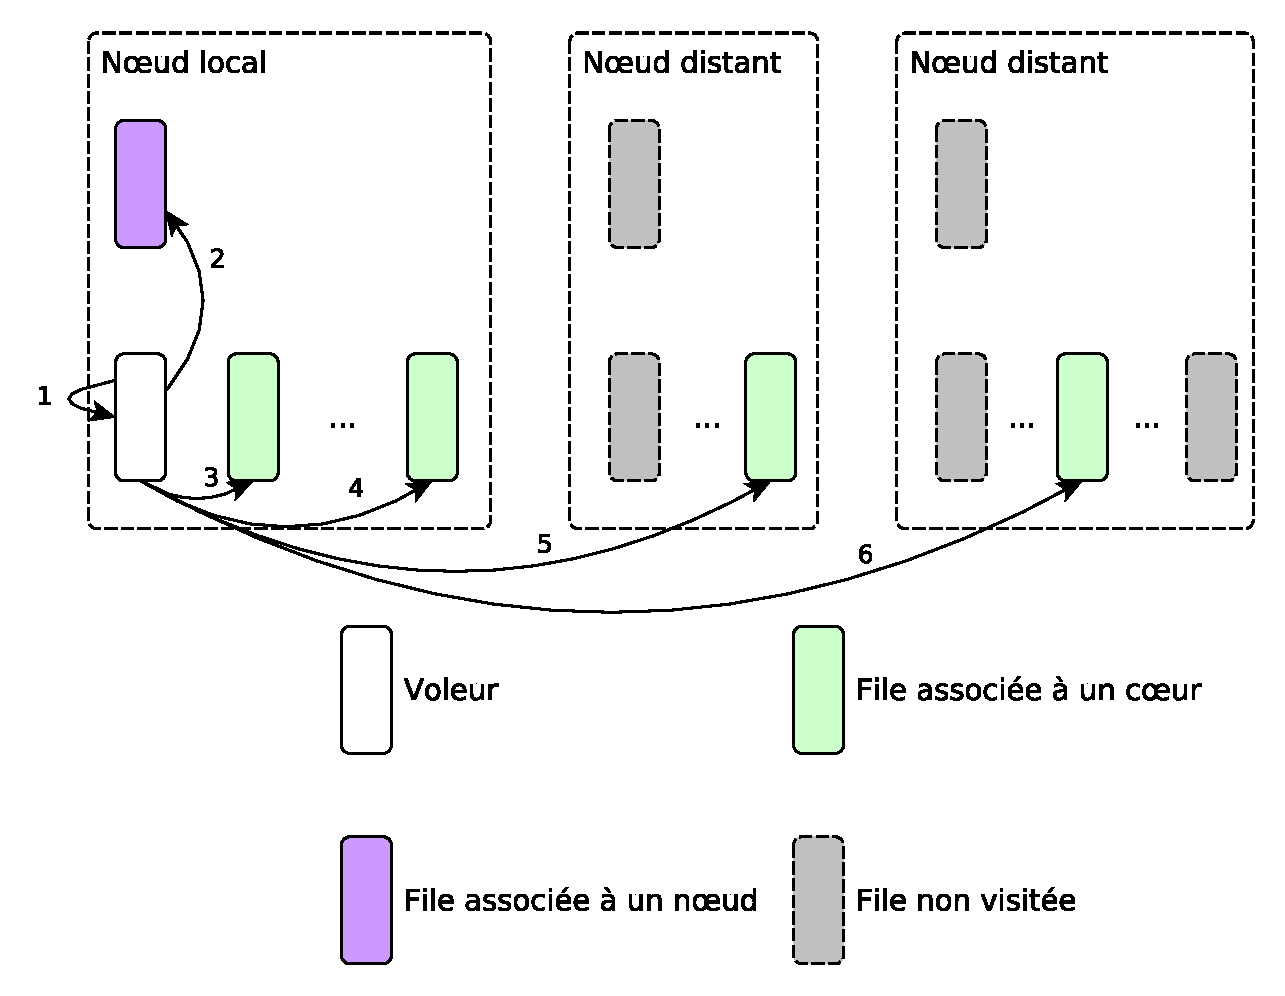
\includegraphics[width=0.73\textwidth]{steal_strategies_proc}
  \caption{Illustration de la stratégie \emph{sProc}, avec l'ordre de visite des files}\label{fig:openmp:runtime:steal_proc}
\end{figure}

\begin{figure}[h!]
  \centering
  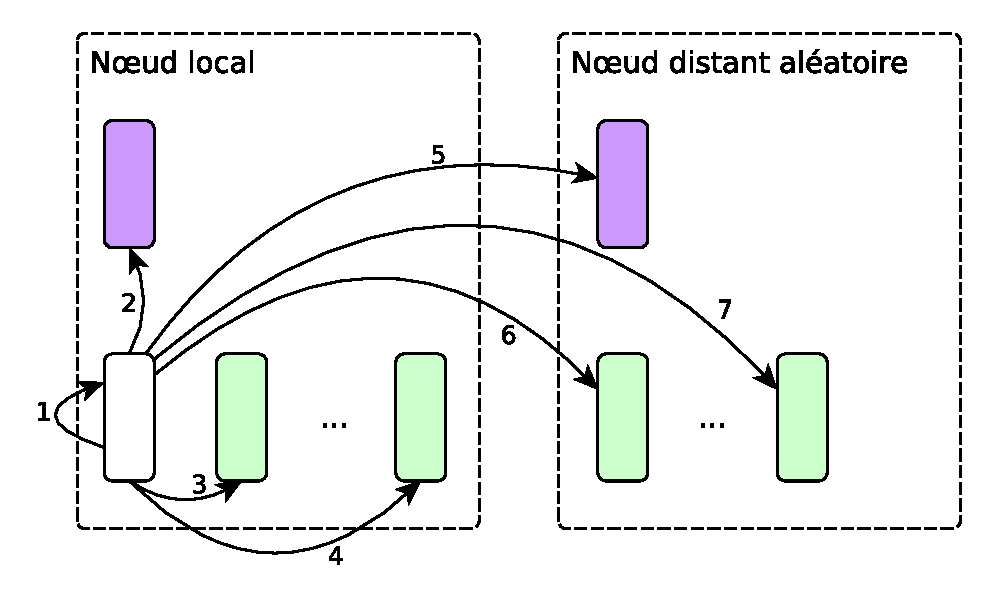
\includegraphics[width=0.6\textwidth]{steal_strategies_numa_proc}
  \caption{Illustration de la stratégie \emph{sNumaProc}, avec l'ordre de visite des files}\label{fig:openmp:runtime:steal_numa_proc}
\end{figure}

\begin{description}
  \item [sProc :] Cette stratégie est illustrée sur la figure~\ref{fig:openmp:runtime:steal_proc}. Le voleur va visiter sa propre file (1), celle de son nœud NUMA (2), puis va parcourir uniquement les files des cœurs en commençant par ses voisins (3, 4), puis en choisissant au hasard parmi les cœurs distant restant (5, 6).
  \item [sNuma :] Le voleur commence par visiter son nœud NUMA, puis les files des cœurs de son nœud, puis uniquement les files des nœuds NUMA distant.
  \item [sProcNuma :] Dans un premier temps le cœur voleur visite sa propre file. Si aucune tâche n'est disponible, il va ensuite visiter les files de tâches des cœurs voisins situés sur le même nœud.
    Si cela échoue de nouveau, il ira voler la file de son nœud NUMA.
    Si cela également, le reste de la topologie sera parcourue de manière similaire : un nœud sera choisi aléatoirement, les files des cœurs puis celle du nœud seront visitées.
  \item [sNumaProc :] Cette stratégie est illustrée sur la figure~\ref{fig:openmp:runtime:steal_numa_proc}~; elle est similaire à la précédente, mais l'ordre de parcours est inversé : après avoir visité sa propre file (1) le voleur regarde d'abord les files des nœuds NUMA (2) avant de regarder les files des cœurs (3, 4). De même que pour la stratégie précédente, le reste de la topologie est parcourue de manière similaire (5, 6, 7).
\end{description}


\subsection{Distribution des tâches d'initialisation}


La section~\ref{sec:openmp:langage:init} décrit comment un utilisateur peut avoir du contrôle sur la distribution des données de son application.
Cela passe par la distribution des tâches d'initialisation, et nécessite donc une modification du support exécutif.

Nous avons implémentés des stratégies additionnelles de placement des tâches prêtes, qui sont prioritaires sur toute autre stratégie décrite dans la section précédent, si une clause |init| est présente.
Elles correspondent directement aux stratégies décrites dans la section~\ref{sec:openmp:langage:init} : \textbf{random}, \textbf{cyclic}, \textbf{cyclicnuma}, et ont naturellement été implémentée en utilisant les files correspondantes de la hiérarchie.

\begin{todo}
  L'intérêt ici était de distinguer ce qu'on propose comme choix à l'utilisateur et comment c'est implémenté derrière.
  Mais bon ça fait un peu maigre comme section...
\end{todo}


\subsection*{Conclusion}

L'ensemble de ces modifications proposent un large choix de paramètres à ajuster pour le support exécutif, et ce n'est pas évident de voir a priori quelle(s) stratégie(s) devraient être privilégiée(s).

Y en a-t-il des meilleures que d'autres quelques soient les circonstances ?
Est-ce que que cela dépend du type d'application ? Du type d'architecture ?
La section suivante propose une évaluation détaillée de l'impact des différents points, et vise à dégager des conseils généraux vis à vis du choix des stratégies.


\section{Évaluation des extensions proposées}\label{sec:contribs:perf_eval}

Nous avons évalué les différentes améliorations proposées dans les sections~\ref{sec:openmp:langage} et~\ref{sec:openmp:runtime} sur les machines idchire et brunch, décrites en détails dans la section~\ref{sec:contribs:machines}.

La section suivante décrit les différents logiciels que nous avons utilisé pour nos expériences, ainsi que les modifications apportées le cas échéant ; et la section~\ref{sec:contribs:perf_eval:resultats} aborde point par point les extensions proposées.
Enfin la section~\ref{sec:contribs:perf_eval:libkomp} discute de l'application de nos idées dans un support exécutif différent, avec également une évaluation de performances.


\subsection{Logiciels}

Les logiciels utilisés pour nos expériences peuvent être divisé en trois catégories~:
\begin{itemize}
  \item Les applications utilisées
  \item Les supports exécutifs
  \item Les bibliothèques externes
\end{itemize}

Les applications et les supports exécutifs utilisées ont pu subire quelques modifications afin d'incorporer les modifications d'OpenMP proposées.
Ces changements sont décrits ci-dessous.
Nous n'avons effectué aucune modification aux bibliothèques externes, mais il est important de faire un point dessus, étant donné qu'une partie des performances peut en dépendre.

\subsubsection{Applications utilisées}

Les applications utilisées pour ces expériences proviennent des KASTORS\footnote{https://gitlab.inria.fr/openmp/kastors, branche 'affinity'}.

Nous avons ajouté une clause \emph{affinity} dans certaines applications~: dans le cas des applications d'algèbre linéaire, les tâches de calculs dépendent d'un ou plusieurs blocs de données. Nous avons ajouté une affinité entre chaque tâche et les données qu'elle écrit.
Dans le cas des applications de type stencil, nous avons ajouté une affinité vers un cœur précis pour les tâches successives.


\subsubsection{Supports exécutifs}


\paragraph{XKAAPI}~: nous avons implémentés les trois types d'extensions proposés dans la section~\ref{sec:openmp:runtime}, à savoir les différentes stratégies de distribution des données, les stratégies de sélection lors du vol de travail, et les stratégies de placement des tâches prêtes.
Ces modifications ont été rassemblées dans une version spécifique de XKAAPI~\footnote{https://scm.gforge.inria.fr/anonscm/git/kaapi/xkaapi.git, branche 'public/europar2016'}.


Nous avons pris comme base de comparaison les supports exécutifs fournis avec les compilateurs existant au moment de nos propositions.

\paragraph{GCC/libGOMP}~: nous avons utilisé la version 5.2.0 comme référence, sans y apporter de modification.

\paragraph{Clang/libOMP}~: nous avons utilisé la version 3.8. Bien que le support exécutif (libOMP) n'ait pas été modifié, le compilateur (Clang) a subit des modifications afin de supporter les clauses décrites dans la section~\ref{sec:openmp:langage}.

\subsubsection{Bibliothèques externes}

\paragraph{BLAS} : les applications d'algèbre linéaire des KASTORS dépendent de la bibliothèque BLAS.
Pour les expériences effectuées dans la section~\ref{sec:contribs:perf_eval:resultats}, nous avons utilisé la bibliothèque OpenBLAS~2.15 pour fournir les noyaux de calculs de base.


\paragraph{hwloc} : cette bibliothèque fournie les informations sur la hiérarchie de la machine, ainsi que des fonctions d'allocation de mémoire selon différentes politique (voir section~\ref{sec:context:os:lib}). Nous avons utilisé la version 1.11.0.

\paragraph{numactl} : nous avons utilisé \emph{numactl} pour certaines courbes de référence. \emph{numactl} est fourni par libNUMA ; nous avons utilisé la version par défaut fourni par le fabricant de la machine.


\subsection{Résultats}\label{sec:contribs:perf_eval:resultats}

\subsubsection{Impact de la distribution des données}

\begin{figure}[ht]
  \centering
  \includegraphics[width=\textwidth]{graph_distrib_data_idchire}
  \caption{Performances des différentes stratégies pour Cholesky en fonction de la distribution de données (N=32768, BS=512)}\label{fig:contribs:perf_eval:distrib-idchire}
\end{figure}

\subsubsection{Impact de l'affinité, et étude comparative des stratégies}

\begin{figure}[ht]
  \centering
  \includegraphics[width=\textwidth]{graph_all_strat_idchire}
  \caption{Performances des différentes stratégies pour Cholesky (N=32768, BS=512)}\label{fig:contribs:perf_eval:eval-strategies}
\end{figure}

\begin{figure}[ht]
  \centering
  \includegraphics[width=\textwidth]{graph_details_qr_cholesky_idchire}
  \caption{Comparaison de trois stratégies sur QR et Cholesky, en fonction de la taille de matrice}\label{fig:contribs:perf_eval:eval-qr-cholesky}
\end{figure}

\begin{todo}
GRAPHE : 5.5.2, Cholesky : (presque non-)impact stratégies affinité sur brunch/idkat
\end{todo}

\subsubsection{Affinité vers des cœurs}

\begin{figure}[ht]
  \centering
  \includegraphics[width=\textwidth]{jacobi_scale_iomp_komp}
  \caption{Performances de Jacobi en fonction de la version et du support exécutif}\label{fig:contribs:perf_eval:eval-jacobi}
\end{figure}

\subsection{Portage dans un autre support exécutif}\label{sec:contribs:perf_eval:libkomp}

\subsubsection{Description}

\subsubsection{Évaluation}

/!\ pour ces xp les versions de gcc/clang ont changé, ainsi que les BLAS !

\begin{todo}
  Il faut aussi comparer ça au simulateur. Peut être plus simplement faire une section à part.

  Vu que c'est principalement effectué avec le nouveau libkomp, peut être mettre ça dans une section suivant celle du "portage" vers le runtime intel.

  À discuter de où on met ça...
\end{todo}



\section{Dicussions et conclusion}


\begin{todo}

parler du fait qu'on pourrait avoir plus d'info, pour prendre de meilleures décisions

on pourrait tester de nouvelles heuristiques à travers un simulateur (ref chapitre 6)

\end{todo}







% This chapter should include
%\begin{itemize}
  %\item HPC ? (OpenMP (with ref to the "main" chapter for details), other existing languages)
\cite{openmp40}, OpenMP 4.0

\cite{openmp45}, OpenMP 4.5

\cite{Marowka2004}, OpenMP-oriented applications for distributed shared memory architectures
  %\item NUMA (with ref to the "main" chapter)
  %\item task + Workstealing (with ref to the "main" chapter)

\cite{cilk5}, CILK

\cite{Tchiboukdjian2010}, A Work Stealing Scheduler for Parallel Loops on Shared Cache Multicores

\part{Related work}

Lorem Ipsum blablabla
%Ce premier chapitre présente brièvement le contexte de cette thèse en section~\ref{sec:intro:contexte}. Puis, nous détaillons les problématiques de recherche en section~\ref{sec:intro:problematique}. Nous présentons les principales contribution de ce travail en section~\ref{sec:intro:demarche}. Ensuite, nous présentons notre cadre applicatif en section~\ref{sec:introduction:digitalhome} et enfin, nous détaillons le plan de ce manuscrit en section~\ref{sec:intro:plan}.

\begin{itemize}
  \item OpenMP
  \item NUMA
  \item Workstealing
\end{itemize}


%\begin{savequote}[6cm]
%<< truc
%\qauthor{Test}
%\end{savequote}

\chapter{Utilisation et amélioration d'OpenMP}\label{chap:contrib:openmp}
\chaptertoc


%\input{tex/OpenMP on numa}
% Big section to describe how we use/extend OpenMP to exploit these architectures

% - Description of OpenMP language (tasking and such)
% - Description of OpenMP runtime

% - Motivating examples for our works using current OpenMP

% - Missing to improve things
%    - What we implemented
%    - What remains

Ce chapitre regroupe les différentes contributions que nous avons faites spécifiquement dans le contexte d'OpenMP.
Cela inclu tout d'abord une suite de benchmarks, KASTORS, regroupant un ensemble de programmes implémentés à l'aide des tâches avec dépendances d'OpenMP, et décrite dans la section~\ref{sec:openmp:kastors}.
Nous décrivons ensuite des extensions dédiées à l'amélioration de la localité des données dans la section~\ref{sec:openmp:langage}.
La section~\ref{sec:openmp:runtime} aborde les modifications faites au niveau du support exécutif pour qu'il puisse avoir une vision hiérarchique de la machine, et qu'il puisse exploiter les informations fournies par les extensions du langage OpenMP proposées.
Enfin toutes ces propositions sont évaluées dans la section~\ref{sec:contribs:perf_eval}.

\section{Préambule : une suite de benchmarks pour OpenMP~4.0, les KASTORS}

\subsection{Motivation pour une nouvelle suite de benchmarks}

Le support pour les applications à base de flots de données dans OpenMP est arrivé avec la version 4.0, qui est sortie au démarrage de cette thèse.
Nous n'avions donc pas d'applications de référence pour utiliser les fonctionnalités ajoutées dans OpenMP, et nous avons donc décidé d'introduire une suite de benchmarks - les KASTORS~\cite{Virouleau2014} - spécifiquement orientée vers ces fonctionnalités, en étendant et regroupant certaines applications existantes.

Il existe évidemment plusieurs suites de benchmarks à destination des architectures à mémoire partagée : d'une part pour les applications à base de tâches indépendantes et utilisant OpenMP~3.0, et d'autre part pour les applications à base de flots de données, mais écrites dans des langages différents.

Parmi les benchmarks populaire ciblant spécifiquement OpenMP, on peut citer la Barcelona OpenMP Task Suite~\cite{Duran2009} (BOTS), proposant des applications à base de tâches OpenMP~3.0 afin d'évaluer le comportement d'OpenMP en fonction de la manière de générer les tâches et de la répartition de la charge de travail.
Nous avons d'ailleurs adapté certaines de leurs applications - SparseLU et Strassen - dans les KASTORS, dont nous parlons plus en détails dans les sections~\ref{sec:kastors:sparselu} et~\ref{sec:kastors:strassen}

Parmi les benchmarks ciblant des modèles de programmations à base de tâche avec dépendances, on peut principalement nommer les PLASMA~\cite{Kurzak2013}.
Cette bibliothèque développée à ICL/UTK met à disposition un grand nombre d'algorithmes d'algèbre linéaire dense, optimisés pour les architectures multi-coeurs.

Nous avions donc assez d'éléments de base pour construire un ensemble d'applications, avec en tête les objectifs suivant :
\begin{itemize}
  \item Rassembler et proposer une suite d'applications exploitant les dépendances introduites avec OpenMP~4.0
  \item Comparer la version utilisant des flots de données à la version utilisant des synchronisations explicites. Le but étant de montrer que le support exécutif peut gérer les synchronisations plus finement, et par conséquent améliorer les performances sans changer l'algorithme.
  \item Avoir une base adaptée pour développer les extensions présentées dans les sections~\ref{sec:openmp:langage} et~\ref{sec:openmp:runtime}.
\end{itemize}

Les sections suivantes décrivent les différents applications de la suite : d'où ils viennent, comment nous les avons étendu pour utiliser les dépendances de données, ainsi que comment nous les avons intégrés.


\subsection{Description des applications}

Les applications suivantes proviennent de différentes suites de benchmarks, et ont été modifiées afin d'utiliser les dépendances de données plutôt que d'autres moyen de synchronisation.

\subsubsection{Factorisations de Cholesky, QR, et LU}

Ces trois applications ont été adaptées des PLASMA.
Dans les PLASMA plusieurs implémentations de chaque algorithme sont disponibles, utilisant soit un ordonnancement statique, soit un ordonnancement dynamique.
Les algorithmes à ordonnancement dynamique sont construit sur le support exécutif QUARK~\cite{YarKhan2011}, qui utilise un modèle avec dépendances de données pour ordonnancer les tâches.

Les trois algorithmes que nous avons sélectionné sont les factorisations de Cholesky, QR, et LU, respectivement nommés DPOTRF, DGEQRF, et DGETRF dans PLASMA.
Ils opèrent tous sur des matrices de nombres flottant à double précision (type |double|).

L'implémentation initiale utilise plusieurs niveaux de wrappers, avec packing et unpacking de paramètres à chaque niveau, ce qui affecte la lisibilité du code et augmente grandement le risque d'erreur.

Les listings~\ref{lst:kastors:dyn} et~\ref{lst:kastors:dyn-omp} montrent respectivement la version dynamique originale, et les transformation que l'on a fait pour porter le code en OpenMP~4.0.
Dans la version originale, la function |wrapper_blas_function| effectue l'unpacking des paramètres avant d'appeler la vraie fonction BLAS/LAPACK sur laquelle elle est construite.
La transformation en OpenMP~4.0 a donné lieu au retrait de plusieurs niveau d'encapsulation, ce qui facilite la lecture du code, la maintenabilité du code, et enlève le besoin de gérer ces paramètres.

\begin{lstlisting}[caption=Format de l'algorithme dynamique,label=lst:kastors:dyn]
wrapper_algorithm_dynamic_call(...) {
  // code séquentiel
  for (...)
    QUARK_Insert_Task(wrapper_blas_function, packed_parameters);
  // code séquentiel
  for (...)
    QUARK_Insert_Task(
        wrapper_another_blas_function,
        packed_parameters);
  // code sequentiel
}
\end{lstlisting}
\begin{lstlisting}[caption=Format de l'algorithme OpenMP,label=lst:kastors:dyn-omp]
algorithm_call(...) {
    // code séquentiel
    for (...)
#pragma omp task depend(inout:array[...])
        blas_function(...);
    // code séquentiel
    for (...)
#pragma omp task depend(inout:array[...])
        another_blas_function(...);
    // code séquentiel
}
\end{lstlisting}


\subsubsection{Jacobi}

C'est un algorithme de type Stencil : c'est un algorithme itératif, et à chaque itérations les différents éléments d'un tableau sont mis à jour en suivant la même formules dépendant généralement des éléments voisins.

En pratique cet algorithme résout l'équation de Poisson sur le carré unitaire [0,1]x[0,1], qui est divisé en une grille de NxN points espacés régulièrement.
Le noyau de calcul principal est un Stencil à 5 points, en 2 dimensions.
Ce noyau est appliqué successivement jusqu'à ce qu'une convergence soit détectée.

Nous avons implémenté deux versions bloquées de ce noyau, en utilisant d'une part des tâches sans dépendances, et d'autre part des tâches avec dépendances.

\subsubsection{SparseLU}\label{sec:kastors:sparselu}

Cette application calcule la factorisation LU d'une matrice creuse.
Nous avons modifié l'implémentation originale des BOTS pour ajouter des dépendances de données.
Ces modifications sont décrites dans les listings~\ref{lst:kastors:sparseLU} et~\ref{lst:kastors:sparseLU-deps}.

\begin{lstlisting}[caption=LU utilisant des tâches indépendantes,label=lst:kastors:sparseLU]
for (k=0; k<NB; k++) {
  lu0(M[k*NB+k]);
  for (j=k+1; j<NB; j++)
#pragma omp task untied shared(M)
    fwd(M[k*NB+k], M[k*NB+j]);

  for (i=k+1; i<NB; i++)
#pragma omp task untied shared(M)
    bdiv(M[k*NB+k], M[i*NB+k]);

#pragma omp taskwait

  for (i=k+1; i<NB; i++)
    for (j=k+1; j<NB; j++)
#pragma omp task untied shared(M)
      bmod(M[i*NB+k],
           M[k*NB+j],
           M[i*NB+j]);
#pragma omp taskwait
}
\end{lstlisting}

\begin{lstlisting}[caption=LU utilisant des tâches avec dépendances,label=lst:kastors:sparseLU-deps]
for (k=0; k<NB; k++) {
#pragma omp task untied shared(M)\
    depend(inout: M[k*NB+k:BS*BS])
  lu0(M[k*NB+k]);
  for (j=k+1; j<NB; j++)
#pragma omp task untied shared(M)\
    depend(in: M[k*NB+k:BS*BS])\
    depend(inout: M[k*NB+j:BS*BS])
    fwd(M[k*NB+k], M[k*NB+j]);

  for (i=k+1; i<NB; i++)
#pragma omp task untied shared(M)\
    depend(in: M[k*NB+k:BS*BS])\
    depend(inout: M[i*NB+k:BS*BS])
    bdiv(M[k*NB+k], M[i*NB+k]);

  for (i=k+1; i<NB; i++)
    for (j=k+1; j<NB; j++)
#pragma omp task untied shared(M)\
   depend(in: M[i*NB+k:BS*BS])\
   depend(in: M[k*NB+j:BS*BS])\
   depend(inout: M[i*NB+j:BS*BS])
    bmod(M[i*NB+k],M[k*NB+j],M[i*NB+j]);
}
\end{lstlisting}

\subsubsection{Strassen}\label{sec:kastors:strassen}

L'application Strassen utilise des décompositions de matrices pour calculer le produit de grandes matrices denses.
De manière similaire à SparseLU, nous avons modifié l'implémentation des BOTS pour ajouter du parallélisme au niveau des additions dans l'algorithme, et nous avons exprimé des dépendances de données plutôt que d'utiliser une synchronisation à base de |taskwait|.

\subsection{Discussions et perspectives}

Nous avons évalué l'intérêt des tâches avec dépendances comparé aux tâches indépendantes dans l'article publié à IWOMP2014~\cite{Virouleau2014}.
Les expériences ont été mené sur toutes les applications avec plusieurs supports exécutifs.
Les résultats ont montrés que l'utilisation des dépendances n'était jamais négatif pour les performances, et induisait en fait une amélioration dans la majorité des cas que nous avons testé.
Cela a pu confirmer que les supports exécutifs pouvaient gérer les synchronisations finement, éliminant ainsi les inactivités des threads dues aux |taskwait|.

D'autres part, ces applications et expériences ont permises de mettre en évidence d'autres limitations des tâches OpenMP.

\begin{figure}[ht]
  \centering
  \includegraphics[width=\textwidth]{jacobi_scale_noaff}
  \caption{Comparaison des performances de Jacobi sur idchire, avec une taille de matrice de 49152}\label{fig:contribs:openmp:kastors:jacobi-motiv}
\end{figure}

La figure~\ref{fig:contribs:openmp:kastors:jacobi-motiv} regroupe une comparaison de l'application de jacobi en fonction de la version implémentée (à base de boucles ou de tâche avec dépendances) et du support exécutif, effectuée sur idchire.
La scalabilité de l'application en elle même est limitée, mais il n'y a pas de raison, a priori, qu'il y ait une dégradation de performances de l'application avec l'augmentation du nombre de cœurs.
Jacobi est une application stencil, et chacune des tâches successives (ou groupe d'itérations pour la version à base de boucles) dépend énormément de la réutilisation du cache L2~: la structure de tâches ne permet pas d'exprimer ce genre de <<dépendances>>, lors de l'ordonnancement certaines tâches vont se faire voler et briser la localité du cache L2, introduisant une grosse dégradation des performances.

Ce problème pourrait être résolu si l'on pouvait exprimer une \emph{affinité} entre une tâche et un cœur de la machine, par exemple.
De plus les résultats de la section~\ref{sec:contribs:apps:cholesky:carton} ont montrés l'importance de la proximité des données pour les différents noyaux de Cholesky, ce qui représente une autre motivation pour la proposition d'une clause permettant l'expression d'une \emph{affinité} entre une tâche et un élément de la machine.

La section suivante aborde ce point, et la section~\ref{sec:contribs:perf_eval} décrit les résultats obtenus à partir des KASTORS étendus avec nos propositions.


\section{Amélioration de l'expressivité du langage}\label{sec:openmp:langage}

Nous avons proposé plusieurs extensions au langage et à l'API d'OpenMP, dont le but général est de faciliter le travail du support exécutif pour maintenir la proximité entre une tâche et ses données au cours de l'exécution du programme.

\subsection{Description du besoin}

Dans un contexte où l'on souhaite améliorer le contrôle sur les tâches et leurs données, OpenMP~4.0 ne propose que deux fonctionnalités~: les |OMP_PLACES| et |OMP_PROCBIND|, mais cela n'a d'effet que sur le placement des threads sur la topologie, et non sur les tâches qui leur sont attribuées.
Il n'y a rien au sein d'OpenMP qui permet d'exprimer une relation entre une tâche et une donnée ou une partie de la topologie de la machine.

En dehors d'OpenMP, les programmeurs utilisent généralement des bibliothèques ou outils externes dans le but de contrôler le placement des données, tels que MAi~\cite{Pousa2009} et MaMi~\cite{Broquedis2010a}.
L'efficacité de certaines approches peut être remise en cause (comme dans le cas de \emph{numactl}), et les approches utilisant une bibliothèque externe peuvent être relativement intrusives.

Nous avons donc introduit deux types de constructions dans OpenMP~: d'une part un moyen de contrôler la distribution initiale des données manipulées par les tâches, et d'autres part un moyen d'associer les tâches à ces données (ou mieux, à n'importe quelle partie de la machine).

\subsection{Contrôle de la distribution des données}\label{sec:openmp:langage:init}

Utiliser une initialisation séquentielle des données de son application peut avoir des conséquences dramatiques sur les performances, tout spécialement lorsque l'on cible des machines NUMA.
Les données se retrouvent dans ce cas sur un unique nœud, dont le bus mémoire va être complètement saturé lorsque les cœurs de tous les autres nœuds vont avoir besoin des données.

Classiquement les programmeurs effectuent l'allocation et l'initialisation des données de manière séquentielle, et utilisent \emph{numactl} pour en faire la distribution.

Ici on va supposer que, de la même manière que le programmeur exprime le parallélisme de son application à base de tâches, il initialise également les données de son application à l'aide de tâches (qu'il est raisonnable de supposer indépendantes) dans une région parallèle séparée.

Dans la plupart des applications que nous avons utilisées nous avons constaté que l'initialisation des données suivait un schéma où l'allocation et l'initialisation de chacun des blocs est fait au fur et à mesure des besoins ou de la construction des structures de données de l'application.

L'initialisation des données devant être groupées ensemble a donc lieu dans une même tâche.
Les solutions de l'état de l'art consistent à allouer, ou migrer, les données initialisées par ces tâches.
Plutôt que d'utiliser une technique similaire, nous allons nous baser sur le principe portable du \emph{first-touch}, décrit dans la section~\ref{sec:context:os}.

Nous proposons ici de distribuer les tâches d'initialisations selon une stratégie choisie par l'utilisateur.
Gérer le placement des tâches est plus efficace et moins couteux que de migrer des données, et permet en fait d'arriver au même résultat~: en distribuant les tâches d'initialisations, on distribue les tâches effectuant le \emph{first-touch} des données, ce qui a pour effet de distribuer physiquement ces données.
Par rapport à \emph{numactl} cela présente également l'avantage de garder sur le même nœud NUMA les données s'étendant sur plusieurs pages.


Pour pouvoir indiquer au support exécutif quelles tâches marquer comme "tâches d'initialisation" et comment gérer leur placement sur la topologie, nous avons mis en place une clause s'appliquant sur une région parallèle~:

\begin{lstlisting}
init(random | cyclic | cyclicnuma)
\end{lstlisting}

Elle indique à l'ordonnanceur de tâches que pour la région parallèle courante les tâches prêtes devraient être distribuées sur la machine en suivant une stratégie :

\begin{description}
  \item [random :]
    distribution aléatoire sur les cœurs de la machine.
  \item [cyclic :]
    distribution de manière cyclique sur les cœurs de la machine.
  \item [cyclicnuma :]
    distribution cyclique sur les nœuds de la machine.
\end{description}


Malgré une restriction dans la manière de réaliser l'initialisation des données de l'application, cet ajout permet au programmeur de spécifier une distribution de données avec une modification minimale du code, et plus efficacement qu'avec les solutions existantes.

Si cette restriction peut être trop forte pour certaines applications, il est aussi possible pour les cas particuliers de spécifier une clause affinité stricte (définie dans la section suivante) sur chacune des tâches d'initialisation.



\subsection{Ajout d'une clause affinité}\label{sec:openmp:langage:affinity}

Pour permettre d'exprimer une association entre une tâche et une donnée (ou un élément de la topologie), nous avons proposé l'introduction du mot clé |affinity| dans le langage OpenMP, qui a été présentée lors du Workshop International sur OpenMP (IWOMP) en 2016~\cite{Virouleau2016b}.
Comme constaté dans le chapitre~\ref{chap:contrib:characterization} et souvent mentionné dans la littérature, un point clé pour obtenir de bonnes performances sur des architectures NUMA est de garantir la proximité entre une tâche et ses ressources.

L'objectif de cette clause est donc de permettre à l'utilisateur de pouvoir spécifier un lien privilégié - une \emph{affinité} - entre une tâche et un élément de l'architecture.
On distingue donc trois types d'affinité que le programmeur pourrait avoir besoin d'exprimer :

\begin{description}
    \item [affinité à un thread :]
      le support exécutif devrait essayer d'ordonnancer la tâche sur le thread donné.
    \item [affinité à un nœud NUMA :]
      le support exécutif devrait essayer d'ordonnancer la tâche sur n'importe
      quel thread du nœud NUMA donné.

    \item [affinité à une donnée :]
      quand une tâche devient prête pour l'exécution, le support exécutif devrait
      l'ordonnancer sur n'importe quel thread attaché au nœud NUMA sur lequel
      la donnée a été physiquement allouée.
\end{description}

De plus, le programmeur peut indiquer si cette affinité est \emph{stricte}, indiquant que la tâche \textbf{doit} s'exécuter sur la ressource indiquée.
Si le programmeur n'indique pas une affinité stricte, l'ordonnanceur peut décider d'exécuter la tâche sur une ressource différente, pour équilibrer la charge de calcul par exemple.

Cette extension visant les constructions de type tâche, elle a été implémentée comme une nouvelle clause pour la directive |task|. La syntaxe proposée est la suivante~:

\begin{lstlisting}
affinity([node | thread | data]: expr[, strict])
\end{lstlisting}

Dans tous les cas l'expression |expr| est un entier naturel, mais en fonction du type d'affinité l'entier est interprété d'une manière spécifique :

\begin{description}
  \item [thread :]
    |expr| est interprétée comme un id de thread. On définit ici la notion d'id de thread comme l'indice du thread au sein des |OMP_PLACES| pour la \textit{team} OpenMP courante.
    Voici une illustration, en prenant une exécution sur quatre threads avec comme valeur |OMP_PLACES="{2},{5},{8},{9}"| :
    \begin{itemize}
      \item Les quatre \emph{threads} qui constituent la \emph{team} vont être ici placés sur quatre \emph{cœurs} de la machine d'indice |2|, |5|, |8|, et |9|.
      \item Les \emph{threads} étant toujours numérotés à partir de |0| dans une \emph{team}, la correspondance entre thread et cœur sera donc la suivante~: le thread d'indice |0| sera donc placé sur le cœur |2|, le thread d'indice |1| sera placé sur le cœur |5|, et ainsi de suite.
    \end{itemize}
  \item [node :]
    |expr| est interprétée comme un id de nœud NUMA. Comme pour le cas précédent, la notion d'id est définie relativement aux places de la \textit{team} OpenMP courante.
    En reprenant l'exemple précédent, supposons que les cœurs 2,5,8, et 9 sont physiquement situés sur 2 nœuds NUMA différents. Il y aura alors 2 nœuds NUMA déduits des places, et les ids utilisés pourront être 0 ou 1.
  \item [data :]
    |expr| est interprétée comme une adresse mémoire. Si le nœud NUMA associé à la donnée ne peut être déterminé, le nœud utilisé par défaut est le nœud local.
\end{description}

Si |expr| désigne une ressource hors limites, la valeur considérée par le support exécutif est prise modulo le nombre de ressources correspondantes.

\subsection{Extension des fonctions du support exécutif}

Si les points précédents décrivent des extensions directement au niveau des constructions OpenMP, il est également important de pouvoir fournir dynamiquement certaines informations au programmeur au cours de l'exécution du programme.
Dans ce but nous avons également ajouté quelques fonctions à l'API d'OpenMP, dont le but est de fournir des informations à propos de l'architecture et de la \emph{team} OpenMP courante :

\begin{lstlisting}
// Retourne le nombre de nœuds NUMA dans la team
int omp_get_num_nodes(void);

// Retourne le nœud NUMA sur lequel
// la tâches est actuellement exécutée
int omp_get_node_num(void);

// Retourne le nœud NUMA sur lequel la donnée a été allouée
int omp_get_node_from_data(void *ptr);
\end{lstlisting}

Ces fonctions retournant des informations spécifiques à une \emph{team} OpenMP, elles ne peuvent être appelées qu'au sein d'une région parallèle.
Sur les machines sans support NUMA, nous considérons que tous les threads sont sur un unique nœud NUMA.

Nous avons également rendu accessible l'ajout d'affinité sur une tâche à une fonction de l'API :
\begin{lstlisting}
void omp_set_task_affinity(omp_affinitykind_t k,
                           uintptr_t ptr, int strict);
\end{lstlisting}
Cette fonction aura un impact sur la prochaine tâche créée dans la région.
Les paramètres de la fonction correspondent aux paramètres de la clause :

\begin{description}
  \item [omp\_affinitykind\_t k] peut être soit |omp_affinity_thread|, |omp_affinity_node|, ou |omp_affinity_data|.
  \item [uintptr\_t ptr] correspond à une expression désignant la ressource.
  \item [int strict] indique si l'affinité est stricte (|strict != 0|) ou non (|strict == 0|).
\end{description}


\subsection{Notes d'implémentation}

Les extensions ont été implémentées dans le compilateur Clang\footnote{https://gitlab.inria.fr/openmp/clang}, en nous basant sur la version~3.9.

Pour intégrer ces extensions, nous avons dans un premier temps étendu différentes parties du \emph{frontend} de Clang~: la partie en charge de l'analyse syntaxique, pour permettre la compréhension des nouvelles clauses et l'enrichissement de l'arbre syntaxique abstrait avec les informations présentes~;
et la partie en charge de l'analyse sémantique afin d'appliquer certaines restrictions sur les clauses (telles que les constructions sur lesquelles elles peuvent être appliquées, ou le type des données attendu).

Dans un second temps nous avons étendu la génération de code, en ajoutant différents point d'entrée dans l'ABI et en passant les données présentes dans l'arbre.

L'ajout des nouveaux points d'entrées dans l'ABI signifie qu'il faut également rajouter leur prise en compte dans le support exécutif, et que du code (contenant des affinités) compilé par notre version modifiée du compilateur n'est pas compatible avec des supports exécutifs n'implémentant pas ces points d'entrée.


L'extension du support exécutif et l'utilisation des informations fournies par le programmeur sont décrites dans la section suivante.

\section{Extension du support exécutif}\label{sec:openmp:runtime}

Cette partie complète la section précédente, puisqu'elle se concentre sur l'exploitation des informations fournies par l'utilisateur, ainsi que sur la prise en compte des architectures NUMA côté support exécutif.

Ces extensions ciblent des supports exécutifs fonctionnant par vol de travail (voir section~\ref{sec:context:runtimes:ws}), et ont été implémenté dans Kaapi ainsi que libKOMP (TODO: ref aux sections décrivant ça ?).

\subsection{Hiérarchiser le support exécutif}

La modification la plus importante consiste à hiérarchiser les files de tâches pour le vol de travail, puisque c'est là dessus que ce base l'ordonnancement.

Des outils tels que hwloc permettent de donner des informations sur la hiérarchie, nous avons donc des informations précises sur quel cœur est placé physiquement sur quel nœud NUMA, et nous avons donc pu mettre en place une hiérarchie dans les files de tâches :

\begin{itemize}
  \item Chaque cœur possèdent deux files de tâches : une publique, dans laquelle les autres cœurs peuvent venir voler ; et une privée, dans laquelle tout le monde peut venir ajouter des tâches, mais seul le cœur propriétaire peut venir voler.
  \item Chaque nœud possèdent également deux files de tâches, suivant le même principe que précédemment. Pour la file privée, seuls les cœurs situés sur le nœud NUMA propriétaire peuvent venir voler des tâches.
\end{itemize}

Nous avons également fait en sorte d'allouer la mémoire manipulée par les différentes files sur le nœud NUMA sur lequel cette file est située.



\subsection{Heuristiques basées sur la localité des données}\label{sec:contrib:ws:heuristics}

Comme décrit dans la section~\ref{sec:context:runtimes:ws}, le vol de travail repose sur deux étapes essentielles : la sélection d'une file de tâches lors du vol, et le choix d'une file lorsqu'une tâche devient prête.

Les deux sections suivantes décrivent les modifications que nous avons mis en place dans le support exécutif, dans l'objectif de prendre en compte le côté NUMA de l'architecture.
Ces travaux ont été publiés à EuroPar 2016~\cite{Virouleau2016b}.


\subsubsection{Distribution des tâches prêtes : stratégies de \emph{placement}}
\label{sec:openmp:runtime:push}

Nous introduisons quatre stratégies différentes pour le placement des tâches prêtes, vis à vis des files de tâches hiérarchiques définies dans la section précédente.
Deux d'entre elles sont indépendantes des données, alors que les deux autres prennent en compte les informations fournies par l'utilisateur via la clause |affinity| décrite dans la section~\ref{sec:openmp:langage:affinity}, ou à défaut utilisent des informations issues des dépendances de données.

\begin{description}
  \item [pLoc :] le processeur responsable du placement de la tâche place celle ci dans sa propre file - \emph{\textbf{p}lacement\textbf{Loc}al}.
  \item [pLocNum :] la stratégie agie de manière similaire à la précédente, à ceci près que le processeur place celle ci dans la file de son nœud NUMA - \emph{\textbf{p}lacement\textbf{Loc}al\textbf{Num}a}.
  \item [pNumaW :] le processeur responsable du placement de la tâche regarde si une affinité de donnée est spécifiée, si aucune affinité n'est présente, il utilise une des dépendances en écriture de la tâche comme affinité.
Il détermine ensuite le nœud NUMA sur lequel a été allouée la donnée, et place la tâche dans la file du nœud correspondant.
  \item [pNumaWLoc :] la stratégie agie de manière similaire à la précédente, mais si le nœud NUMA déterminé correspond au nœud NUMA du processeur courant, alors la tâche est poussée dans la file du processeur directement.
\end{description}

Un détail distingue les deux premières stratégies des deuxx secondes : dans le cas des stratégies |pLoc| et |pLocNum|, le placement initial des données n'est pas pris en compte, alors que les stratégies |pNumaW| et |pNumaWLoc| utilisent toutes deux les informations sur l'allocation physiques des données manipulées par la tâche.

\subsubsection{Équilibrage de charge dynamique : stratégie de \emph{sélection}}
\label{sec:openmp:runtime:select}


Nous avons implémenté un ensemble de stratégie de sélection de files de tâches, qui ont conscience de la topologie de l'architecture sur laquelle est exécutée le programme.

Les deux premières sont similaires aux travaux effectués par Olivier et al.~\cite{Olivier2012} :
\begin{description}
  \item [sRand :] sélection aléatoire d'une file parmi les files des cœurs.
  \item [sRandNuma :] sélection aléatoire d'une file parmi les files des nœuds.
\end{description}

Ces deux stratégies pourront servir de base de comparaison avec les stratégies suivantes, prenant en compte les deux niveaux de hiérarchie disponibles, ainsi que la notion de << voisinage >> entre cœurs.

\begin{figure}[t!]
  \centering
  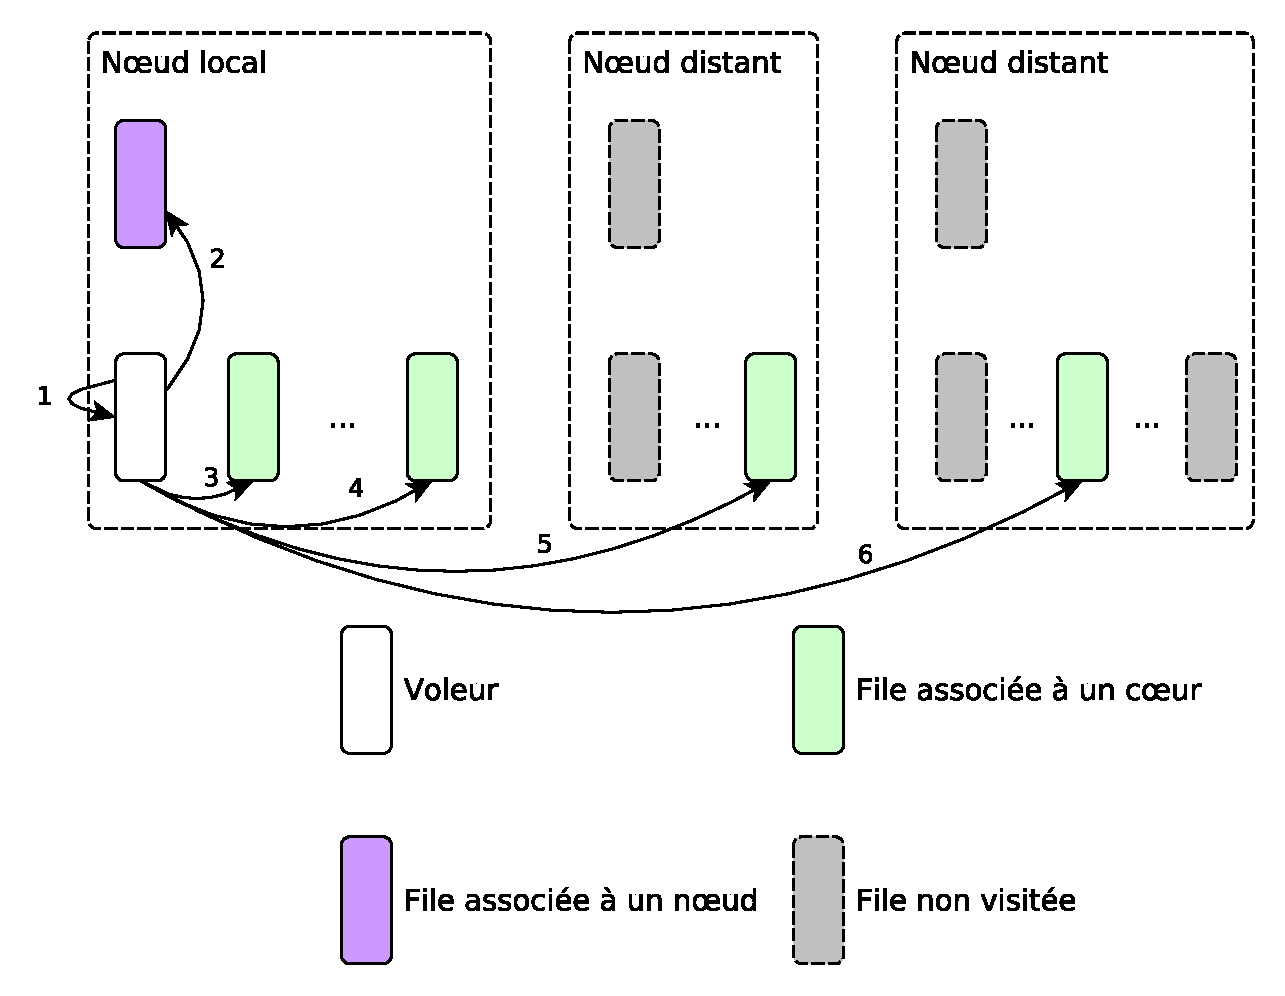
\includegraphics[width=0.73\textwidth]{steal_strategies_proc}
  \caption{Illustration de la stratégie \emph{sProc}, avec l'ordre de visite des files}\label{fig:openmp:runtime:steal_proc}
\end{figure}

\begin{figure}[h!]
  \centering
  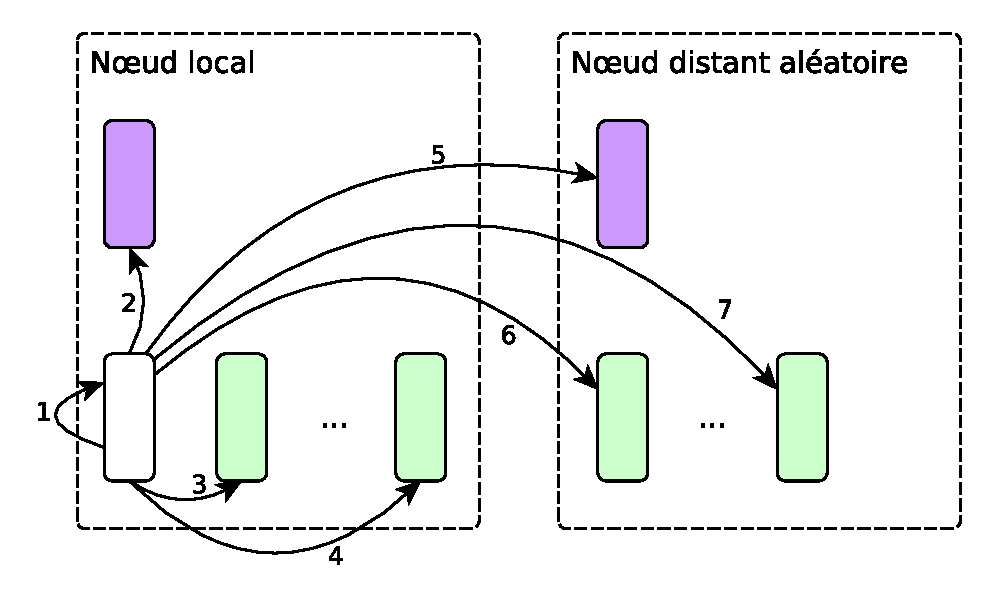
\includegraphics[width=0.6\textwidth]{steal_strategies_numa_proc}
  \caption{Illustration de la stratégie \emph{sNumaProc}, avec l'ordre de visite des files}\label{fig:openmp:runtime:steal_numa_proc}
\end{figure}

\begin{description}
  \item [sProc :] Cette stratégie est illustrée sur la figure~\ref{fig:openmp:runtime:steal_proc}. Le voleur va visiter sa propre file (1), celle de son nœud NUMA (2), puis va parcourir uniquement les files des cœurs en commençant par ses voisins (3, 4), puis en choisissant au hasard parmi les cœurs distant restant (5, 6).
  \item [sNuma :] Le voleur commence par visiter son nœud NUMA, puis les files des cœurs de son nœud, puis uniquement les files des nœuds NUMA distant.
  \item [sProcNuma :] Dans un premier temps le cœur voleur visite sa propre file. Si aucune tâche n'est disponible, il va ensuite visiter les files de tâches des cœurs voisins situés sur le même nœud.
    Si cela échoue de nouveau, il ira voler la file de son nœud NUMA.
    Si cela également, le reste de la topologie sera parcourue de manière similaire : un nœud sera choisi aléatoirement, les files des cœurs puis celle du nœud seront visitées.
  \item [sNumaProc :] Cette stratégie est illustrée sur la figure~\ref{fig:openmp:runtime:steal_numa_proc}~; elle est similaire à la précédente, mais l'ordre de parcours est inversé : après avoir visité sa propre file (1) le voleur regarde d'abord les files des nœuds NUMA (2) avant de regarder les files des cœurs (3, 4). De même que pour la stratégie précédente, le reste de la topologie est parcourue de manière similaire (5, 6, 7).
\end{description}


\subsection{Distribution des tâches d'initialisation}


La section~\ref{sec:openmp:langage:init} décrit comment un utilisateur peut avoir du contrôle sur la distribution des données de son application.
Cela passe par la distribution des tâches d'initialisation, et nécessite donc une modification du support exécutif.

Nous avons implémentés des stratégies additionnelles de placement des tâches prêtes, qui sont prioritaires sur toute autre stratégie décrite dans la section précédent, si une clause |init| est présente.
Elles correspondent directement aux stratégies décrites dans la section~\ref{sec:openmp:langage:init} : \textbf{random}, \textbf{cyclic}, \textbf{cyclicnuma}, et ont naturellement été implémentée en utilisant les files correspondantes de la hiérarchie.

\begin{todo}
  L'intérêt ici était de distinguer ce qu'on propose comme choix à l'utilisateur et comment c'est implémenté derrière.
  Mais bon ça fait un peu maigre comme section...
\end{todo}


\subsection*{Conclusion}

L'ensemble de ces modifications proposent un large choix de paramètres à ajuster pour le support exécutif, et ce n'est pas évident de voir a priori quelle(s) stratégie(s) devraient être privilégiée(s).

Y en a-t-il des meilleures que d'autres quelques soient les circonstances ?
Est-ce que que cela dépend du type d'application ? Du type d'architecture ?
La section suivante propose une évaluation détaillée de l'impact des différents points, et vise à dégager des conseils généraux vis à vis du choix des stratégies.


\section{Évaluation des extensions proposées}\label{sec:contribs:perf_eval}

Nous avons évalué les différentes améliorations proposées dans les sections~\ref{sec:openmp:langage} et~\ref{sec:openmp:runtime} sur les machines idchire et brunch, décrites en détails dans la section~\ref{sec:contribs:machines}.

La section suivante décrit les différents logiciels que nous avons utilisé pour nos expériences, ainsi que les modifications apportées le cas échéant ; et la section~\ref{sec:contribs:perf_eval:resultats} aborde point par point les extensions proposées.
Enfin la section~\ref{sec:contribs:perf_eval:libkomp} discute de l'application de nos idées dans un support exécutif différent, avec également une évaluation de performances.


\subsection{Logiciels}

Les logiciels utilisés pour nos expériences peuvent être divisé en trois catégories~:
\begin{itemize}
  \item Les applications utilisées
  \item Les supports exécutifs
  \item Les bibliothèques externes
\end{itemize}

Les applications et les supports exécutifs utilisées ont pu subire quelques modifications afin d'incorporer les modifications d'OpenMP proposées.
Ces changements sont décrits ci-dessous.
Nous n'avons effectué aucune modification aux bibliothèques externes, mais il est important de faire un point dessus, étant donné qu'une partie des performances peut en dépendre.

\subsubsection{Applications utilisées}

Les applications utilisées pour ces expériences proviennent des KASTORS\footnote{https://gitlab.inria.fr/openmp/kastors, branche 'affinity'}.

Nous avons ajouté une clause \emph{affinity} dans certaines applications~: dans le cas des applications d'algèbre linéaire, les tâches de calculs dépendent d'un ou plusieurs blocs de données. Nous avons ajouté une affinité entre chaque tâche et les données qu'elle écrit.
Dans le cas des applications de type stencil, nous avons ajouté une affinité vers un cœur précis pour les tâches successives.


\subsubsection{Supports exécutifs}


\paragraph{XKAAPI}~: nous avons implémentés les trois types d'extensions proposés dans la section~\ref{sec:openmp:runtime}, à savoir les différentes stratégies de distribution des données, les stratégies de sélection lors du vol de travail, et les stratégies de placement des tâches prêtes.
Ces modifications ont été rassemblées dans une version spécifique de XKAAPI~\footnote{https://scm.gforge.inria.fr/anonscm/git/kaapi/xkaapi.git, branche 'public/europar2016'}.


Nous avons pris comme base de comparaison les supports exécutifs fournis avec les compilateurs existant au moment de nos propositions.

\paragraph{GCC/libGOMP}~: nous avons utilisé la version 5.2.0 comme référence, sans y apporter de modification.

\paragraph{Clang/libOMP}~: nous avons utilisé la version 3.8. Bien que le support exécutif (libOMP) n'ait pas été modifié, le compilateur (Clang) a subit des modifications afin de supporter les clauses décrites dans la section~\ref{sec:openmp:langage}.

\subsubsection{Bibliothèques externes}

\paragraph{BLAS} : les applications d'algèbre linéaire des KASTORS dépendent de la bibliothèque BLAS.
Pour les expériences effectuées dans la section~\ref{sec:contribs:perf_eval:resultats}, nous avons utilisé la bibliothèque OpenBLAS~2.15 pour fournir les noyaux de calculs de base.


\paragraph{hwloc} : cette bibliothèque fournie les informations sur la hiérarchie de la machine, ainsi que des fonctions d'allocation de mémoire selon différentes politique (voir section~\ref{sec:context:os:lib}). Nous avons utilisé la version 1.11.0.

\paragraph{numactl} : nous avons utilisé \emph{numactl} pour certaines courbes de référence. \emph{numactl} est fourni par libNUMA ; nous avons utilisé la version par défaut fourni par le fabricant de la machine.


\subsection{Résultats}\label{sec:contribs:perf_eval:resultats}

\subsubsection{Impact de la distribution des données}

\begin{figure}[ht]
  \centering
  \includegraphics[width=\textwidth]{graph_distrib_data_idchire}
  \caption{Performances des différentes stratégies pour Cholesky en fonction de la distribution de données (N=32768, BS=512)}\label{fig:contribs:perf_eval:distrib-idchire}
\end{figure}

\subsubsection{Impact de l'affinité, et étude comparative des stratégies}

\begin{figure}[ht]
  \centering
  \includegraphics[width=\textwidth]{graph_all_strat_idchire}
  \caption{Performances des différentes stratégies pour Cholesky (N=32768, BS=512)}\label{fig:contribs:perf_eval:eval-strategies}
\end{figure}

\begin{figure}[ht]
  \centering
  \includegraphics[width=\textwidth]{graph_details_qr_cholesky_idchire}
  \caption{Comparaison de trois stratégies sur QR et Cholesky, en fonction de la taille de matrice}\label{fig:contribs:perf_eval:eval-qr-cholesky}
\end{figure}

\begin{todo}
GRAPHE : 5.5.2, Cholesky : (presque non-)impact stratégies affinité sur brunch/idkat
\end{todo}

\subsubsection{Affinité vers des cœurs}

\begin{figure}[ht]
  \centering
  \includegraphics[width=\textwidth]{jacobi_scale_iomp_komp}
  \caption{Performances de Jacobi en fonction de la version et du support exécutif}\label{fig:contribs:perf_eval:eval-jacobi}
\end{figure}

\subsection{Portage dans un autre support exécutif}\label{sec:contribs:perf_eval:libkomp}

\subsubsection{Description}

\subsubsection{Évaluation}

/!\ pour ces xp les versions de gcc/clang ont changé, ainsi que les BLAS !

\begin{todo}
  Il faut aussi comparer ça au simulateur. Peut être plus simplement faire une section à part.

  Vu que c'est principalement effectué avec le nouveau libkomp, peut être mettre ça dans une section suivant celle du "portage" vers le runtime intel.

  À discuter de où on met ça...
\end{todo}



\section{Dicussions et conclusion}


\begin{todo}

parler du fait qu'on pourrait avoir plus d'info, pour prendre de meilleures décisions

on pourrait tester de nouvelles heuristiques à travers un simulateur (ref chapitre 6)

\end{todo}



\section{Architectures à mémoire partagée}\label{sec:context:numa}


Les architectures à mémoire partagée ont subit des changements majeurs liés à l'évolution des processeurs.
L'augmentation du nombre de cœurs par processeur a introduit des problèmes d'accès à la mémoire centrale : dans une architecture composée d'une unique mémoire, plusieurs cœurs cherchant à accéder à la mémoire vont rentrer en concurrence et introduire de la contention et donc des délais dans l'accès à la mémoire, ce qui pénalise formtement les performances.

Pour pallier ce problème, les constructeurs ont divisé la mémoire centrale en plusieurs parties physiquement distinctes, appelées \emph{nœuds}.
Le nœud NUMA est le composant de base pour une architecture NUMA.
Chaque nœud est constitué d'une partie de la mémoire centrale, d'un contrôleur local d'accès à ce bloc mémoire, ainsi que d'un certain nombre de cœurs de calcul.
L'ensemble des nœuds de la machine sont ensuite reliés entre eux par un réseau d'interconnexion.
La topologie de l'interconnexion ne permet généralement pas d'avoir des nœuds équidistants, ce qui introduit une hiérarchie mémoire.

Malgré le fait que les différentes parties de l'architecture soient physiquement séparées, le système d'exploitation voit l'ensemble comme une unique machine.

Nous décrivons dans un premier temps les caractéristiques techniques communes d'un processeur multicœur d'un nœud dans les sections~\ref{sec:context:numa:cache}, et~\ref{sec:context:numa:node}, puis celles des systèmes d'interconnexion des nœuds dans la section~\ref{sec:context:numa:interconnect}.
Elles ont une influence directe sur le comportement du nœud au sein de la machine.

\subsection{Caches des processeurs}\label{sec:context:numa:cache}

Le cache est une mémoire pour laquelle le temps d'accès est bien meilleur que pour la mémoire centrale, mais dont la capacité est beaucoup plus restreinte. Il peut être spécifique à un cœur du processeur, ou partagé par plusieurs d'entre eux.

\subsubsection{Fonctionnement}

Au niveau des accès le fonctionnement d'un cache est légèrement différent de celui de la mémoire centrale : plutôt que de lire uniquement un octet, c'est généralement une partie fixe de la mémoire contenant cet octet qui est chargée.
On appelle cette quantité une \emph{ligne de cache}, et un exemple de taille standard pour une ligne de cache est 64 octets (8 nombres réels double précision).

Lorsqu'une instruction demande le chargement d'une valeur située en mémoire, le contrôleur du cache reçoit la requête du processeur, détermine la ligne de cache correspondante à partir de l'adresse demandée, et effectue l'une des deux opérations suivantes :
\begin{description}
  \item [Cache hit :] si la ligne correspondante est déjà présente dans le cache la donnée est directement retournée au cœur.
  \item [Cache miss :] si la ligne n'est pas présente le contrôleur de cache va charger la valeur depuis la mémoire centrale vers le cache, et retourner la valeur au cœur.
\end{description}

%(je vire ça vu qu'on ne parle de niveaux de cache que plus tard) Si le cœur a accès à plusieurs niveaux de cache, la requête est transférée au niveau supérieur, et seul le dernier niveau effectue la requête à la mémoire centrale.
Une fois qu'une ligne est chargée dans le cache, elle n'y reste pas de manière permanente, plusieurs raisons décrites ci-après peuvent entraîner son \emph{éviction} du cache :

\begin{itemize}
  \item Le maintien de la cohérence : lorsqu'un cœur modifie une ligne de cache dans son propre cache, cette même ligne est \emph{invalidée} dans les caches des autres processeurs qui en disposent d'une version.
Si un processeur essaie de faire un accès sur une ligne invalidée, elle sera rechargée depuis la mémoire centrale, générant un \emph{cache miss}.
  \item Le dépassement de la capacité du cache : il est assez commun que l'ensemble des données manipulées par le programme ne tienne pas dans le cache.
Lorsqu'une requête est effectuée sur une ligne, qu'elle n'est pas présente dans le cache, et que le cache est plein, le contrôleur choisira une ligne à évincer du cache pour faire de la place à la nouvelle ligne.
Le choix de la ligne à évincer est un sujet très étudié, et le prochain paragraphe revient sur les politiques d'éviction communément utilisées.
  \item Le conflit d'adresse : dans certains modèle de caches, certaines lignes correspondant à des adresses mémoires doivent être stockées dans le même emplacement du cache.
    Si elles sont requises alternativement pendant l'exécution du programme, elles se sortiront mutuellement du cache.
    Ce problème dépend directement de l'\emph{associativité} du cache, qui est traitée dans le paragraphe suivant.
\end{itemize}



\subsubsection{Associativité}

Le cache ne pouvant être suffisamment grand pour contenir toute la mémoire, il faut pouvoir déterminer l'association entre l'adresse d'une ligne dans la mémoire centrale et son emplacement dans le cache.
Il y a trois grandes catégories d'associativité utilisées par les caches :
\begin{itemize}
  \item Les caches à association directe (\emph{direct-mapped cache}) : dans ce système, chaque ligne de la mémoire est associée à exactement un emplacement dans le cache.
    Ce système est simple, propose le meilleur temps de réponse, mais est peu prévisible et à taille identique est moins efficace que les deux autres catégories.
  \item Les caches complètement associatifs (\emph{fully associative cache}) : dans ce système, chaque ligne de la mémoire peut être associée à n'importe quel emplacement dans le cache.
    Cela permet de maximiser l'utilisation de l'espace disponible, mais cela induit un coût supplémentaire pour déterminer l'association entre une ligne et son emplacement.
  \item Les caches N-associatifs (\emph{N-way associative cache}) : ce système est un compromis entre les deux précédents.
    Chaque ligne de la mémoire peut être associée à exactement N emplacements dans le cache.
    Cela implique un certain nombre d'opérations sur les adresses des lignes, et l'espace pris par le composant ainsi que le temps d'accès moyen dépend directement de la valeur de N.
\end{itemize}

Hill et al.~\cite{Hill1989} (Table III) illustre l'impact de l'associativité sur la proportion de cache miss et catégorise son origine (conflit d'adresse, défaut de capacité du cache, chargement normal de la donnée).
Cela permet de dégager deux observations : d'une part qu'augmenter l'associativité permet de diminuer les cache miss.
D'autre part que les défauts de cache ayant une forte associativité sont quasi exclusivement dus à la capacité du cache, alors que pour les caches à association directe les conflits d'adresse sont une part non négligeable des cache miss.

\subsubsection{Niveaux de caches}

Il y a en général 3 niveaux de cache dans ces architectures :
\begin{itemize}
  \item L1 : C'est le cache le plus "proche" du CPU, mais aussi le plus petit - typiquement quelques Ko. Il est généralement découpé en deux parties distinctes : une partie pour les instructions, une autre pour les données.
  \item L2 : Ce cache est physiquement plus éloigné du processeur et présente une latence d'accès plus importante que le L1, mais propose une plus grande capacité de mémoire. Il a un ordre de grandeur de quelques centaines de Ko.
  \item L3 : Ce cache est généralement le cache de dernier niveau - \emph{Last Layer Cache (LLC)} - sur un processeur. La latence pour y accéder est plus importante que le L2, mais sa capacité est bien supérieure, pouvant en général atteindre plusieurs Mo.
\end{itemize}

En fonction des fabricants, ces caches peuvent être soit \emph{inclusifs} (c'est-à-dire que toutes les données présentes dans le L1 sont également présentes dans le L2), ou \emph{exclusifs} (c'est-à-dire qu'une donnée est garantie de n'être présente que dans l'un des caches).

Au sein d'un nœud, le L3 est généralement partagé par tous les cœurs, alors que les caches L1 et L2 sont spécifiques à un cœur.

\begin{figure}[ht]
  \centering
  \includegraphics{processor_small}
  \caption{Schéma d'un processeur multicœurs}\label{fig:context:schema-caches}
\end{figure}

La figure~\ref{fig:context:schema-caches} décrit la hiérarchie typique d'un processeur multicœurs que l'on peut trouver sur un nœud NUMA.
Dans cet exemple, le processeur dispose de 8 cœurs, et chaque cœur dispose d'une cache L1 indépendant pour les données et les instructions (32 Ko chacun), d'un cache L2 (256 Ko), et d'un cache L3 partagé avec 7 autres cœurs (20 Mo).


En général les développeurs d'applications pour le HPC accordent beaucoup d'attention à l'optimisation de leur application, pour que les parties de code séquentiel critiques utilisent des données qui puissent être contenues dans le L1/L2.
De même, beaucoup d'optimisations au sein des compilateurs visent également cet objectif.

Lorsqu'il s'agit de cibler des architectures NUMA, on va tout particulièrement s'intéresser au L3, qui représente la mémoire la plus rapide accessible par tous les cœurs d'un même nœud.

\begin{todo}
TODO : ref + paragraph sur les caches configurables du ryzen.
Pas trouvé de ref sur le ryzen parlant de cache configurable, mais j'ai trouvé Jenga : http://people.csail.mit.edu/sanchez/papers/2017.jenga.isca.pdf
\end{todo}

\begin{table}[ht]
\def\arraystretch{1.5}
\centering
\begin{tabular}{|c||c|c|c|c|}\hline
  Cache & \multicolumn{2}{c|}{Intel Sandy Bridge} & \multicolumn{2}{c|}{Intel Broadwell}  \\ \cline{2-5} 
 & Latence & Bande passante & Latence & Bande passante \\ \hline
 L1 & 1.6 ns & 16 Go/s & 1.8 ns & 32 Go/s \\ \hline
 L2 & 5.0 ns & 14 Go/s & 5.4 ns & 17 Go/s \\ \hline
 L3 & ~20 ns & 8 Go/s & ~24 ns & 9 Go/s \\ \hline
 RAM & ~90 ns & 4 Go/s & ~140 ns & 7 Go/s \\ \hline
\end{tabular}
\caption{Tableau synthétiques des latences et bande passante en fonction du niveau de cache et du processeur}\label{tab:synthese-processeurs}
\end{table}

Afin de donner un ordre d'idée des latences et bande passantes sur les différents processeurs, le tableau~\ref{tab:synthese-processeurs} récapitule les chiffres en fonction de la génération du processeurs.
Les mesures ont été faites à l'aide de l'outil LMbench~\cite{McVoy1996}. Pour la latence, les temps considérés sont ceux du benchmark |lat_mem_rd| avec un accès aléatoire à la mémoire.
Pour la bande passante les temps considérés sont ceux du benchmark |bw_mem|, en utilisant un équivalent de |memcpy|.
Pour la latence, tout effet potentiel du prefetcher est annulé par l'utilisation de \emph{pointer chasing} (l'adresse de la case suivante à charger est située dans la case courante), ce qui n'est pas le cas pour la bande passante.

Comme on peut le voir sur ces chiffres, le coût d'accès à la mémoire principale est prohibitif par comparaison aux différents caches, y compris le L3.
Les différentes caractéristiques de ces processeurs et des machines sur lesquels ils sont intégrés seront étudiées en détails dans la section~\ref{sec:contribs:machines}.

\subsubsection{Politiques d'éviction}

Le choix de la ligne de cache à remplacer lorsque le cache est plein a un impact direct sur les performances, et les politiques de remplacement ont été très étudiées par les différents acteurs de la communauté académique et industrielle.

La politique optimale serait de remplacer la ligne qui sera réutilisée le plus tard, mais ce genre de clairvoyance est impossible à implémenter en pratique.
Un certain nombre d'alternatives ont donc été imaginées, et sont décrites ci-après :
\begin{itemize}
  \item Random : cette politique choisi une ligne à remplacer au hasard. Sa simplicité la rend simple à implémenter en pratique, et a notamment été utilisée dans les processeurs ARM Cortex-R~\cite{ARM-Cortex-R}.
  \item First-In First-Out : comme son nom l'indique, la ligne remplacée est la première qui est rentrée dans le cache parmi celles présentes.
  \item Least Recently Used (LRU) : dans cette politique, chaque ligne dispose de plusieurs bits représentant la date de la dernière utilisation de cette ligne. La ligne remplacée est celle ayant été utilisée il y a le plus longtemps.
  \item Pseudo-LRU : cette politique offre une version dégradée permettant de gérer des caches de grandes tailles.
Lorsque l'associativité du cache dépasse un certain seuil, le coût d'implémentation de LRU devient trop important~\cite{Kedzierski2010}, l'alternative proposée par les politiques pseudo-LRU est donc de remplacer une ligne parmi celles utilisées il y a le plus longtemps.
Cela permet de limiter le nombre de bits nécessaire pour tracer les lignes à remplacer potentielles.
  \item Autres politiques adaptatives : dans le cas spécifique du cache de dernier niveau (LLC), certains fabriquants comme Intel utilisent des politiques adaptatives présentées comme supérieures à Pseudo-LRU, prenant en compte la fréquence à laquelle sont utilisées certaines lignes de caches.
    \emph{Dynamic Re-Referency Interval Prediction} en est un exemple, qui a été présenté parmi d'autres par Jaleel et al.~\cite{Jaleel2010}.
\end{itemize}

La politique pseudo-LRU semble être la plus utilisée par les fabricants de processeurs tous niveaux de cache confondus. Al-Zoubi et al.~\cite{Al-Zoubi2004} proposent une évaluation complète et détaillée de l'impact des politiques d'éviction en fonction de l'associativité du cache, justifiant le choix des constructeurs.



\subsection{Autres caractéristiques matérielles des processeurs}\label{sec:context:numa:node}

En plus des caches qui nous intéresseront tout particulièrement dans la suite de ce manuscrit, les processeurs ont également d'autres composants matériels dont il est important d'avoir conscience, mais qui ont une place plus limitée dans le contexte de cette thèse : il s'agit des instructions vectorielles et de l'hyperthreading, décrit ci-après.

\subsubsection{Instructions vectorielles}\label{sec:context:numa:simd}

Le concept de vectorisation est l'action d'appliquer une même instruction sur plusieurs données (ou un \emph{vecteur} de données) nécessitant la même opération.
Ce type d'instructions est appelée SIMD, pour \emph{Single Instruction Multiple Data}.

Afin d'illustrer ce point, il suffit d'imaginer que l'on souhaite additionner deux vecteurs d'entiers :
\begin{lstlisting}
int vecteur_a[8] = { 1 };
int vecteur_b[8] = { 1 };
int addition[8];
for (int i = 0; i < 8; i++) {
  addition[i] = vecteur_a[i] + vecteur_b[i];
}
\end{lstlisting}

Exécuter la boucle complète effectuerait 8 additions sur des entiers.
En supposant que la largeur des registres (et des instructions) du processeur est de 64 bits, et que la taille d'un |int| est 32 bits, on "gaspillerait" en fait 32 bits par addition.

Étant donné que l'on souhaite effectuer la même opération (une addition), sur des éléments indépendants du tableau, on peut alors aisément grouper deux additions successives dans la même instruction : il suffit de mettre un entier de 32 bits sur la partie haute du registre, et un deuxième entier sur la partie basse, d'effectuer l'instruction, et de faire l'opération inverse pour stocker le résultat dans le tableau.
De plus la vectorisation permet au processeur d'optimiser la décomposition de l'instruction en micro opérations et donc l'utilisation du pipeline.
Au final on divise le nombre d'itérations, mais aussi le nombre d'accès mémoire et d'opérations par 2.


\begin{todo}
  j'ai pas trouvé la ref des procs vectoriels sur ACM, (re)demander à Thierry
\end{todo}

Des extensions au jeu d'instructions x86 ont été créées afin de pouvoir opérer sur des éléments plus larges que 64 bits, et la plupart des architectures des processeurs récents utilisent des registres plus larges que le type le plus large en C (|long long|, 64 bits).
La première d'entre elles, SSE (\emph{Streaming SIMD Extensions}), a été introduite par Intel dès 1999 et a évolué régulièrement, agrandissant progressivement la taille des registres jusqu'à l'extension AVX-512, permettant d'effectuer des instructions sur des registres de 512 bits.

La plupart des processeurs actuels (depuis les Sandy Bridge d'Intel, et les Bulldozer d'AMD, en 2011) supportent au moins l'extension AVX avec des registres de 128 bits.

\subsubsection{Hyperthreading}

Chaque cœur possède un certain nombre d'UAL (Unité Arithmétique et Logique) qui lui sont privées. Lorsqu'il est en attente d'une donnée de la mémoire centrale, ces UALs ne sont pas utilisées, et des cycles CPU sont donc "perdus" à ne rien faire.

Afin de maximiser l'utilisation de ces ressources, certains processeurs Intel sont équipés de la technologie \emph{hyperthreading}.
Le concept est assez simple : avoir deux cœurs logiques (\emph{hyperthreads}) associés à un seul cœur physique.
De cette manière lorsqu'un thread est en attente sur une donnée (par exemple lors d'un chargement d'une donnée depuis la mémoire), le second peut profiter des UALs disponibles.

Pour des tâches peu gourmandes en ressources ou utilisant beaucoup de données, cela peut effectivement se traduire par un gain de performances, mais pour le cas des applications HPC il faut regarder le type d'applications utilisées pour savoir si on peut espérer un gain ou non.
En particulier les caches L1 et L2 sont partagés par les deux hyperthreads, donc si le code séquentiel généré est optimisé pour les tailles de caches correspondant, exécuter le même type de code séquentiel sur deux hyperthreads peut entrainer du \emph{cache trashing}.
Au meilleur des cas l'hyperthreading améliorera les performances mais ne sera pas forcément très efficace, atteignant par exemple entre 2.3 et 3.3 de speed-up pour 4 hyperthreads par cœur~\cite{Jeffers2016} sur les derniers processeurs d'Intel, les Xeon Phi.
Si l'application est très intensive en calcul et utilise au maximum les UALs, l'hyperthreading n'apportera pas grand chose, voire rien.

L'hyperthreading est généralement une option que l'on peut désactiver dans le BIOS de la machine, ou éviter en plaçant correctement les threads de son application.


\subsection{Interconnexion des nœuds}\label{sec:context:numa:interconnect}

L'une des parties majeures d'une machine NUMA est le système d'interconnexion entre les différents nœuds.
C'est cette partie qui va déterminer à quel point cela va être couteux d'accéder à la mémoire située sur un nœud distant, et donc à quel point l'aspect NUMA de la machine va impacter les performances d'une application.
Dans la majorité des cas, ce système d'interconnexion est \emph{cache-coherent}, c'est à dire que la cohérence de cache est assurée entre les différents nœuds par le matériel, et n'est pas la responsabilité du programmeur ou du support exécutif.
L'impact sur les performances peut être lié à la fois au protocole de cohérence de caches utilisé, ainsi qu'à la topologie de l'interconnexion des nœuds.


\subsubsection{Protocoles de cohérence de cache}

Le nombre de caches utilisés dans une machine NUMA peut être important, et la même ligne de la mémoire peut être présente dans plusieurs caches en même temps.
Il est important que l'état des différentes copies soit cohérent : par exemple si une ligne a été écrite et modifiée, les copies de cette ligne dans les autres caches doivent être mises à jour.

La plupart des protocoles se basent sur un ensemble d'états possibles pour une ligne de cache :

\begin{description}
  \item [Modified (M) :] la ligne a été modifiée dans le cache. Les données dans cette ligne ne sont donc pas cohérentes avec la mémoire principale. Quand la ligne est évincée, elle doit être écrite dans la mémoire principale.
  \item [Shared (S) :] la ligne est <<propre>> (non modifiée), elle existe dans d'autres caches mais est en lecture seule dans le cache courant. Cette ligne peut être évincée sans autre action.
  \item [Invalid (I) :] la ligne est soit absente du cache courant ou a été invalidé par un autre cache. Elle doit être récupérée depuis la mémoire principale (ou un autre cache qui en possède une copie valide).
\end{description}

Cet ensemble d'états de base forme le protocole \emph{MSI}, qui a ensuite été étendu avec plusieurs autres états :

\begin{description}
  \item [Exclusive (E) :] la ligne est présente uniquement dans le cache courant et elle est <<propre>>.
  \item [Owned (O) :] la ligne est présente dans plusieurs caches dans un état valide, mais seul le cache courant peut y effectuer des modifications.
    Cet état permet de partager des lignes qui ont été modifiées sans passer par une ré-écriture dans la mémoire centrale : le cache qui possède la ligne est responsable de fournir une version à jour, et d'écrire la ligne dans la mémoire centrale lorsque que la ligne est évincée.
  \item [Forward (F) :] cet état est similaire à l'état \emph{Shared}, mais indique au cache courant qu'il est responsable de satisfaire une requête en lecture sur la ligne.
\end{description}

Intel Quick Path Interconnect~\cite{Ziakas2010} (QPI) est le système d'interconnexion utilisé dans les machines d'expérimentation que nous avons utilisé, et qui sont décrites dans la section~\ref{sec:contribs:machines}.
Il implémente le protocole MESIF. Du à l'introduction de l'état \emph{F}, ce protocole est avantageux lorsque la latence de cache à cache est bien plus faible que la latence d'accès à la mémoire principale.

Pour implémenter ce protocole, il existe deux types de mécanismes :

\begin{itemize}
  \item À base de Snooping : chaque cache observe le trafic sur le bus mémoire pour des requêtes qui concerneraient les lignes de caches dont ils possèdent une copie. Un composant dédié peut effectuer un premier filtre pour restreindre le trafic lié au mécanisme de snooping. Néanmoins ce type de mécanismes ne passent pas bien à l'échelle, et aurait du mal à obtenir de bonne performance dans les architectures NUMA, où le nombre de caches est important.

  \item À base de répertoires : la donnée est placée dans un répertoire qui maintien la cohérence entre les caches. Chaque cache ne peut pas accéder directement à la mémoire principale mais doit passer par le répertoire.
\end{itemize}

Le QPI utilise un mix des deux mécanismes : il utilise des \emph{home agents} - comparables à des répertoires - qui sont les principales autorités pour fournir une version du cache depuis la mémoire principale.
Il utilise ensuite du \emph{snooping} pour satisfaire les requêtes des différents \emph{caching agents} (les entités qui possèdent un cache, telles que les processeurs).

Le QPI peut fonctionner avec deux modes de \emph{snooping} :
\begin{description}
  \item [Source snooping :] le \emph{caching agent} envoie la requête à tout le système. Les autres \emph{caching agent} peuvent répondre à la requête s'ils possèdent une version de la ligne de cache dans un état compatible. Le \emph{home agent} responsable de la ligne mémoire doit fournir une copie propre de la ligne de cache si besoin, et résoudre les conflits s'ils apparaissent.
  \item [Home snooping :] le \emph{caching agent} envoie la requête au \emph{home agent}, qui envoie ensuite une requête aux \emph{caching agents} qui possèdent une copie de la ligne et peut commencer à charger la ligne depuis la mémoire. L'un des \emph{caching agents} possédant la ligne et/ou le \emph{home agent} peut ensuite envoyer la réponse.
\end{description}

Le mode \emph{source snooping} a une latence plus faible que le mode \emph{home snooping}, mais passe moins bien à l'échelle.
C'est donc ce dernier qui est le plus adapté à un environnement NUMA, puisqu'il limite le nombre de requêtes envoyés sur le bus mémoire, et économise donc de la bande passante.


\subsubsection{Topologies}
\begin{todo}
  décrire le facteur NUMA et inclure des chiffre (reprendre graphe 2.1.2 plus bas)
\end{todo}

La topologie du système d'interconnexion peut être très différente d'une machine à une autre, et de multiples exemples existent dans les machines commercialisées.
Il existe des topologies plates, où chaque nœud est directement connecté aux autres (TODO: ref graph 2.1.2), des topologies où des couples de nœuds sont groupés entre eux et peuvent passer par un ou deux niveaux d'interconnexion (TODO: ref graph idchire).

Le nombre de rebonds - \emph{hops} - à effectuer avant d'accéder à la mémoire demandée impacte directement la latence et la bande passante, comme le montre le tableau comparatif de la figure~(TODO).

Chiffres :
même noeud: 2.11 GB/s
noeud meme group: 1.50 GB/s
groupe proche: 1.28 GB/s
groupe loin: 1.06 GB/s

GRAPHE : 2.1.2 les chiffres de base !
GRAPHE : 2.1.2 heatmap
GRAPHE : 2.1.2 montrer une version schématique d'une machine NUMA (2 socket, 1 socket/2 nœuds, idchire, knl)



\subsection*{Conclusion}

Cette partie s'est concentrée sur les connaissances de base nécessaires pour comprendre l'interaction entre les différents composants des architectures NUMA.
Le développeur d'application ne va généralement pas influer directement sur ces composants, en revanche il est capital d'avoir conscience des caractéristiques de chacun d'entre eux pour pouvoir expliquer facilement tel ou tel comportement de l'application.

Le premier composant logiciel qui va s'intéresser à la gestion directe du matériel est le système d'exploitation.
La section suivante revient sur les points relatifs à la gestion des architectures NUMA dans le système d'exploitation.


  %\item Related work


%\end{itemize}

\part{Étude approfondie des machines NUMA, et amélioration de leur utilisation à travers OpenMP}



%\begin{savequote}[6cm]
%<< truc
%\qauthor{Test}
%\end{savequote}

\chapter{Caractérisation des architectures NUMA}\label{chap:contrib:characterization}
\chaptertoc

\section{Exécution précise de noyaux}\label{sec:contribs:outil}

Cette partie se concentre sur la présentation de \outil, un outil que nous avons créé afin de faciliter la réalisation d'expériences avec un contrôle précis sur le placement de noyaux à exécuter ainsi que leurs données.
Le but de ces expériences est d'analyser le comportement des parties de calcul critiques aux performances d'une application, sur une architecture donnée.

\subsection{Besoins pour un outil spécifique: \outil}

Il est en général assez facile d'étudier le comportement global d'une application, et d'observer les variations de ce comportement lorsqu'on change certains détails dans l'exécution, comme par exemple via l'utilisation de \emph{numactl}.

En revanche, si l'on connait bien son application, on a envie de pouvoir étudier le comportement précis de certaines de ses parties critiques afin de pouvoir identifier ce qui cause son comportement global.

La suite naturelle de cette identification est de déterminer s'il existe des améliorations possibles pour ce comportement local, et comment l'améliorer en pratique.

Dans le cas d'une application à base de flots de données, chaque partie de l'application est bien identifiée, et correspond à un nœud dans le graphe de tâches.
Toutes les données manipulées par une partie de l'application sont facilement identifiées également, puisqu'il s'agit des connexions entre les nœuds du graphe de tâches.

Dans le contexte d'une machine NUMA, le temps d'exécution d'une tâche dépend à la fois du placement de son exécution, ainsi que du placement de ces données. On a donc envie de pouvoir étudier le comportement individuel de chaque type de tâche en fonction de son placement et du placement des données qu'elle accède.
Une fois cela fait, cela permettra d'identifier des potentielles variations de comportement, et ajuster les heuristiques d'ordonnancement pour prendre en compte ces variations.

Nous n'avons pas trouvé d'outil existant répondant précisément à ce besoin.
BOAST~\cite{Videau2017} est un outil assez proche dans la thématique d'optimisation de noyaux applicatif~: l'utilisateur fourni des noyaux et un ensemble d'optimisations possibles, BOAST en déduit un espace à explorer et va rechercher automatiquement les paramètres optimaux.

Dans notre cas l'objectif n'est pas d'optimiser le code, mais de replacer le noyau applicatif dans une série de situations se présentant au cours de l'exécution réelle de l'application, afin de déterminer des stratégies d'ordonnancement qui pourrait favoriser l'exécution de ce noyau applicatif dans de bonnes conditions.
De fait nous avions également besoin d'un outil qui nous permette de contrôler et faire varier le placement des noyaux et de ses données sur la topologie de la machine, et qui permette une exécution simultanée de noyaux applicatifs.

C'est à ce besoin que répond \outil : une fois que l'utilisateur a isolé les parties critiques de son application, \outil lui permet de définir lesquelles il souhaite exécuter et où, et lui garantir cette exécution, avec un certain nombre de variables observables.

Dans la suite de ce chapitre, on appellera l'ensemble des paramètres décrivant cette expérience un \emph{scenario}.

\subsection{Description d'un scenario}

Ce que l'on appelle ici un \emph{scenario} n'est ni plus ni moins que la description d'une expérience.
Par exemple on pourrait vouloir "observer les performances en gigaflops d'une multiplication de matrices carrées sur le cœur 0 d'une machine".
C'est un scénario simple, et l'exemple que l'on prendra pour illustrer les points un peu plus formel qui vont suivre.

En pratique un scénario est défini par les éléments suivants :
\begin{itemize}
 \item Un ensemble de données et variables~;
 \item Une liste d'actions à effectuer~;
 \item Un ensemble de caractéristiques à observer.
\end{itemize}


Il est important que le format de description d'un scénario soit humainement lisible, et ne conduise pas à une recompilation systématique du programme. C'est donc une description en YAML~\cite{YAML} qui a été choisie.


\paragraph{Modèle d'exécution.}

Le flot d'exécution est le suivant~:
Dans un premier \outil commence par charger le scénario fourni par l'utilisateur, créer les différentes données, et analyser les actions pour déterminer l'ensemble des cœurs physiques qui seront utilisés au cours des actions.
Pour chacun des cœurs utilisés, un thread est créé et attaché à ce cœur. De plus, une file d'actions (FIFO) est créée pour ce thread.
Les actions sont poussées dans les files d'actions correspondantes, dans l'ordre du fichier.
Une fois l'ensemble des actions chargées, les threads exécutent chacun les actions présentes dans leur file, et vont déclencher les mesures de chaque paramètre observé avant et après chaque action.

Une unique primitive de synchronisation est disponible, sous la forme d'une action prédéfinie à insérer dans le scénario~: une barrière sur un ensemble arbitraire de cœurs.


L'architecture de l'outil est donc simple, avec peu de logique relative au contrôle de l'exécution des tâches et à la synchronisation, ce qui permet de minimiser le <<bruit>> lors des expériences.

Les sections suivantes reviennent sur les différentes caractéristiques définissant un scénario, avec des exemples concrets d'utilisation.


\subsubsection{Données et variables}

Elles sont indispensables car c'est là-dessus que vont se baser les actions du scénario.

L'utilisateur doit fournir les noms et types des variables utilisées en paramètre des différents noyaux, elles peuvent être réutilisées par différents noyaux.

\outil ne prend pas en charge l'allocation ou l'initialisation des données. Dans le cas de variables simples comme des constantes, elles peuvent être directement affectées dans le scénario. Dans le cas de variables complexes, l'utilisateur doit déclarer une action d'initialisation (avec ses paramètres) dans \outil, pour pouvoir l'utiliser ensuite dans le scénario pour initialiser les données.
Cette action peut être soit une fonction implémentée comme un module de \outil, soit être un point d'entrée dans une bibliothèque externe.

\outil met néanmoins à disposition une fonction d'allocation ne faisant aucune réutilisation de page, avec une politique explicite d'allocation physique des pages en \emph{first-touch}.


Pour revenir à l'exemple du scénario simple ou l'on souhaite exécuter une multiplication de matrices carrées - |dgemm| - sur un cœur donné, nous avons besoin de trois matrices |a|, |b|, et |c|, ainsi qu'une largeur en nombre d'éléments pour les matrices manipulées, |size|.

Voici concrètement à quoi ressemblerait la déclaration de ces données :

\begin{lstlisting}[language=yaml,caption=Exemple de déclaration de variables,label=lst:tool:data-example]
data:
  - a:
    - type: "double *"
  - b:
    - type: "double *"
  - c:
    - type: "double *"
  - size:
    - type: "int"
    - value: 256
\end{lstlisting}

Nous pouvons voir ici que |size| est initialisée directement, mais les pointeurs |a|, |b|, et |c| seront initialisés plus tard par une action.

\paragraph{Déclarations multiples.}

Il est possible de créer un ensemble de variables en se basant sur un modèle paramétré de nom.
Un nom de variable peut contenir un ensemble de caractères (|[a-zA-Z]+|) encadré par des chevrons (|<>|).
Cet ensemble de caractères est interprété comme un paramètre du nom de la variable, et la déclaration devra alors contenir l'ensemble des valeurs que ce paramètre peut prendre.
L'ensemble des valeurs est soit~: un ensemble d'entier désignant, à la manière d'une boucle, les limites de l'espace d'itération sous la forme |[début, fin, pas]|~; ou bien un ensemble de chaines de caractères qui seront substituées dans le nom de la variable.

L'exemple suivant illustre cette syntaxe en déclarant les variables |a0|, |a2|, |a4|, |a6|, |array_input|, et |array_output|~:

\begin{lstlisting}[language=yaml,caption=Exemple de déclaration de variables paramètrées,label=lst:tool:data-example-for]
data:
  a<i>:
    i: [0, 7, 2]
    type: "double *"
  array_<name>:
    name: ["input", "output"]
    type: "int *"
\end{lstlisting}



\subsubsection{Actions}

C'est là où l'utilisateur décrit effectivement les noyaux exécutés au cours du scénario.
Il indique une série d'actions à exécuter, et avec quels paramètres.

\paragraph{Définition d'une action.}

Les actions peuvent être prédéfinies par \outil, ou encore être implémentées par l'utilisateur comme un module de \outil, ou finalement être un point d'entrée dans une bibliothèque.
Le listing~\ref{lst:tool:declare-action} donne un exemple d'une définition d'action qui serait externe à \outil, où l'on ciblerait la fonction |cblas_dsyrk| de la bibliothèque OpenBLAS.

\begin{figure}[h!]
\begin{lstlisting}[language=yaml,caption=Exemple de définition d'une action externe,label=lst:tool:declare-action]
declare_actions:
  - library: "openblas"
    # Identifiant de l'action
    name: "dsyrk"
    # Point d'entrée dans la bibliothèque
    entry_point: "cblas_dsyrk"
    params:
    - "int"
    - "int"
    - "int"
    - "int"
    - "int"
    - "double"
    - "double *"
    - "int"
    - "double"
    - "double *"
    - "int"
\end{lstlisting}
\end{figure}

\paragraph{Utilisation dans un scénario.}

Un scénario doit contenir une entrée |actions|, qui est le tableau d'actions à réaliser au cours du scénario.
Chaque action peut avoir les caractéristiques suivantes :
\begin{description}
  \item [kernel~:] chaine de caractères identifiant l'action.
    Cet attribut n'a pas de valeur par défaut et est obligatoire.
  \item [core~:] nombre entier indiquant le cœur sur lequel exécuter l'action. Il n'a pas de valeur par défaut, et est obligatoire.
  \item [params~:] liste de variables à passer en paramètre de l'action, leur nom doit correspondre à des données déclarées dans la section précédente.
  \item [repeat~:] nombre entier indiquant le nombre de fois que cette action doit être répétée. La valeur par défaut est 1.
\end{description}

\outil dispose d'une action prédéfinie~: la barrière. Son identifiant est |barrier|, et pour cette action spécifiquement le traitement de l'attribut |core| est un peu différent~: il peut ne pas être spécifié, et auquel cas la barrière sera effectuée sur l'ensemble des cœurs, mais il peut également être un ensemble de cœurs pour restreindre la portée de la barrière.


Si on continue à décrire l'exemple simple d'une multiplication de matrices carrées, il faut que l'on effectue les actions suivantes : l'initialisation de chaque matrice (via une action |init_blas_bloc|, implémentée au préalable par l'utilisateur dans \outil, qui prend en paramètre un pointeur et une largeur de matrice), et le lancement du dgemm une fois que ces matrices sont initialisées.
Afin d'avoir une mesure plus précise du comportement du noyau, on peut indiquer une répétition du noyau, ici on choisit 50 pour l'exemple.

Le listing~\ref{lst:tool:actions-example} montre un exemple réalisant ce scénario.

\begin{figure}[h!]
\begin{lstlisting}[language=yaml,caption=Exemple d'actions à réaliser pour une multiplication de matrice,label=lst:tool:actions-example]
actions:
  - kernel: init_blas_bloc
    params:
    - a
    - size
    core: 0
  - kernel: init_blas_bloc
    params:
    - b
    - size
    core: 0
  - kernel: init_blas_bloc
    params:
    - c
    - size
    core: 0
  - kernel: dgemm
    params:
    - a
    - b
    - c
    - size
    core: 0
    repeat: 50
\end{lstlisting}
\end{figure}

Ici les trois initialisations et le calcul ont lieu sur le même cœur, et sont déroulés dans l'ordre de création, il n'y a donc pas lieu d'utiliser une synchronisation.

\paragraph{Actions paramétrées}

De manière similaire à la déclaration de données, il est possible de paramétrer les actions.
Cela peut être particulièrement pratique dans le cas où l'on souhaite observer l'exécution concurrente de plusieurs noyaux de calcul.

Cela se fait à l'aide d'une action spéciale \emph{for}, qui doit définir plusieurs attributs~: |var|, qui contient le nom de la variable d'itération, et |actions|, qui contient la liste des actions à effectuer.
Pour définir l'espace d'itération, l'utilisateur doit spécifier un et un seul des deux attributs suivants~: |limits|, qui s'exprime sous la forme |[débug, fin, pas]| et permet d'exprimer les limites de la boucles~; ou |values|, qui indique une liste explicite des valeurs que peut prendre la variable.

Le listing~\ref{lst:tool:actions-example-sync} fait une utilisation de cette syntaxe pour exécuter 4 dgemm simultanément sur les cœurs 0, 1, 2, et 3, en ayant au préalable initialisé les données nécessaires.

\begin{figure}[h!]
\begin{lstlisting}[language=yaml,caption=Exemple de déclaration d'actions synchronisées,label=lst:tool:actions-example-sync]
data:
  # Déclaration de a0, a1, a2, a3, etc
  a<i>:
    i: [0, 3, 1]
    type: "double *"
  b<i>:
    i: [0, 3, 1]
    type: "double *"
  c<i>:
    i: [0, 3, 1]
    type: "double *"
actions:
  # Initialise a0, b0, et c0 sur le coeur 0,
  # a1, b1, et c1 sur le coeur 1, etc.
  - for:
      var: name
      values: ["a", "b", "c"]
      actions:
        - for:
            var: i
            limits: [0, 3, 1]
            actions:
              - kernel: init_blas_bloc
                params:
                - <name><i>
                - size
                core: <i>
  # Synchronisation avant de lancer les dgemm
  - kernel: barrier
  # Lancement d'un dgemm sur le coeur 0 utilisant a0, b0, et c0,
  # et d'un dgemm sur le coeur 1 utilisant a1, b1, et c1, etc.
  - for:
      var: i
      limits: [0, 3, 1]
      actions:
        - kernel: dgemm
          params:
          - a<i>
          - b<i>
          - c<i>
          - size
          core: <i>
          repeat: 50
\end{lstlisting}
\end{figure}

Cette syntaxe permet d'exprimer des scénarios relativement complexe de manière compacte.
En revanche simplement exécuter ces actions ne nous donnera pas grand chose, il faut donc définir un ensemble de caractéristiques à observer pendant leur exécution.

\subsubsection{Observateurs}

\outil utilise des \emph{Observateurs} pour enregistrer certaines caractéristiques au cours de la vie du programme.
Un observateur peut avoir plusieurs attributs~:
\begin{description}
  \item [name~:] un identifiant d'observateur existant dans \outil.
  \item [params~:] les paramètres à passer lors de la création de l'observateur.
  \item [kernels~:] une liste d'identifiants d'actions sur lesquelles appliquer cet observateur.
\end{description}

\outil propose de base deux observateurs élémentaires~:

\begin{itemize}
  \item \emph{time}~: le temps passé dans l'action (en millisecondes).
  \item \emph{papi}~: permettant de relever des compteurs de performances à travers PAPI.
\end{itemize}

L'utilisateur peut implémenter lui-même des observateurs additionnels au sein de \outil.
Dans notre cas nous avons implémenté des observateurs spécifiques à certains noyaux d'algèbre linéaire, qui dérivent du temps passé dans l'action et qui indique la performance équivalente en Gflops.

La figure~\ref{lst:tool:watchers-example} illustre à quoi ressemblerait la section du scénario si nous souhaitions observer la performance de dgemm en Gflops, le nombre de cycles, ainsi que le nombre de \emph{cache miss} de niveau 3 pendant l'exécution de chaque dgemm.

\begin{figure}[h!]
\begin{lstlisting}[language=yaml,caption=Exemple de déclaration d'observateurs,label=lst:tool:watchers-example]
watchers:
  - name: flops_dgemm
    # Le nombre de flops dépend de la taille de la matrice,
    # qu'il faut donc donner en paramètre.
    params:
      - size
    kernels:
      - dgemm
  - name: papi
    params:
      - PAPI_TOT_CYC
      - PAPI_L3_TCM
    kernels:
      - dgemm
\end{lstlisting}
\end{figure}

L'ensemble des compteurs à observer étant passé tel quel à PAPI, il est donc de la responsabilité de l'utilisateur de fournir un ensemble de compteurs compatibles entre eux.

L'observation se faisant sur la base d'une seule action, une ligne récapitulative est générée à partir des données des observations.
Si l'utilisateur a indiqué une action avec un |repeat| de 50, il y aura donc 50 lignes avec les valeurs récoltées pour chaque action.

\subsubsection{Notes d'implémentation}

La syntaxe décrite et les fonctionnalités décrites ici sont celles que devraient contenir \outil une fois terminé.
Pour des raisons de temps, un certain nombre de fonctionnalités n'ont pas encore été implémentées~: les syntaxes paramétrées (déclaration de variables et d'actions paramétrées)~; les actions utilisateurs chargées depuis des bibliothèques externes (seules les actions implémentées comme des modules sont utilisables)~; et le filtrage des observateurs par action (le filtrage a lieu en dur dans le code pour le moment).

\subsection{Application et exemples de scénarios}

\outil nous a servi dans deux types de contexte~: pour la caractérisation des machines sur lesquelles nous avons effectuées nos expériences, et pour l'étude détaillées des parties critiques des applications que nous avons utilisées.

La section~\ref{sec:contribs:machines} dresse un profil détaillé des machines et présente une utilisation de \outil pour mesurer certaines caractéristiques de la machine, qui n'aurait pas été facilement mesurable à travers d'autres outils.
La section~\ref{sec:contribs:apps:cholesky} présente une étude de cas de l'une des applications que nous avons utilisé~: la factorisation de Cholesky.
Elle revient sur le fonctionnement de l'outil, les observations préliminaires que nous avons effectué, et la valeur ajoutée qu'a eu \outil dans la compréhension détaillée et l'amélioration des performances de l'application.




\section{Présentation et caractéristiques des machines}\label{sec:contribs:machines}

Nous présentons dans cette sections deux machines NUMA de générations différentes et au caractéristiques assez différentes.
La première, \emph{idchire}, est basée sur des processeurs Intel Sandy Bridge, et possède un nombre important de nœuds NUMA.
La seconde, \emph{brunch}, est basé sur des processeurs Intel plus récents de la génération Broadwell, et dispose d'un nombre assez faible de nœud NUMA.

\subsection{idchire}\label{sec:contribs:machines:idchire}

Cette machine est équipée de 24 processeurs Intel(R) Xeon(R) CPU E5-4640 (Sandy Bridge), cadencés à 2.4 GHz.
Chacun de ce processeurs est associé à 31 Go de RAM pour former un nœud NUMA, ils disposent de 8 cœurs physiques partageant 20 Mo de cache L3 (20-ways associatif).
Chacun des cœur à accès à 32 Ko de cache L1 (données) et 256 Ko de cache L2 (8-ways associatif).

La machine entière dispose donc de 192 cœurs physiques, et de 744 Go de RAM.
Les processeurs Sandy Bridge disposent de l'extension vectorielle AVX, permettant d'effectuer 4 additions et 4 multiplication de nombres flottant à double précision en un cycle, portant le pic de performance théorique de la machine à 3.6 TFLOPs.

\subsubsection{Topologie}

\begin{figure}[ht]
  \centering
  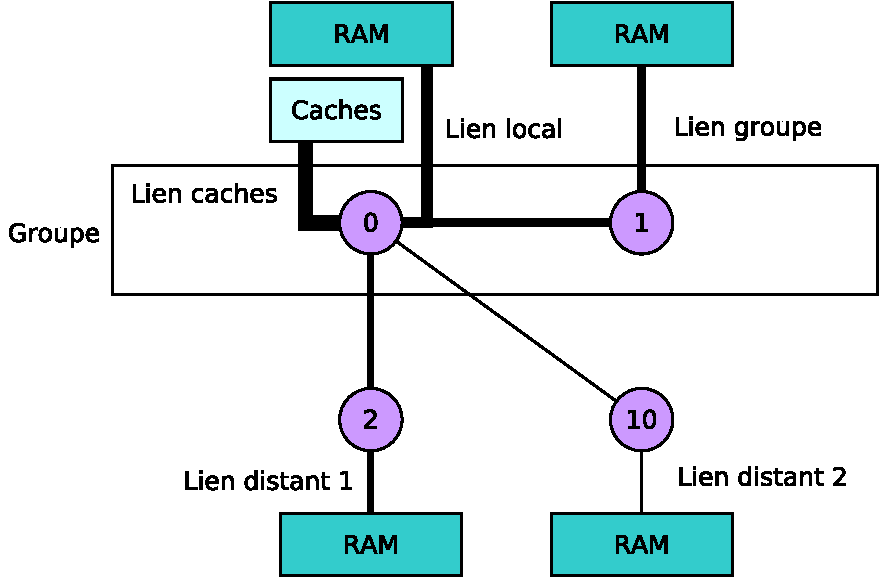
\includegraphics[width=\textwidth]{topo-idchire}
  \caption{Topologie schématique vu du nœud 0}\label{fig:contribs:machines:idchire:topo-liens}
\end{figure}

L'interconnexion des nœuds NUMA est effectué à travers l'Intel \emph{Quick Path Interconnect} (QPI).
La topologie de la machine expose une hiérarchie à plusieurs niveaux, la Figure~\ref{fig:contribs:machines:idchire:topo-liens} présente la hiérarchie de la machine du point de vue du nœud 0.
Chaque nœud est d'abord associé à un autre nœud pour former un groupe. Ces groupes sont ensuite interconnectés entre eux et sont accessibles en deux rebonds maximum dans le système d'interconnexion.
Pour chaque nœud il y a 12 nœuds situés à un rebond, et 10 nœuds situés à deux rebonds.

\begin{figure}[t!]
  \centering
  \includegraphics[width=\textwidth]{heatmap_idchire_memcpy}
  \caption{Carte de la bande passante d'idchire}\label{fig:contribs:machines:idchire:heatmap}
\end{figure}

\begin{figure}[h!]
  \centering
  \includegraphics[width=0.9\textwidth]{link_saturation}
  \caption{Bande passante depuis le nœud 0, en fonction du nombre de threads effectuant une copie et du nœud destination}\label{fig:contribs:machines:idchire:saturation}
\end{figure}


La Figure~\ref{fig:contribs:machines:idchire:heatmap} présente la bande passante nœud à nœud en fonction de la source et de la destination, mesurée à l'aide d'une copie de tableau (|memcpy|) de 200 Mo.
Elle fait apparaître clairement une diagonale où la bande passante est significativement plus grande, illustrant le coût d'un accès mémoire local comparé à un accès distant.

Néanmoins cette simple <<carte>> ne suffit pas à caractériser complètement les temps d'accès aux nœuds NUMA, puisque qu'une seule communication ne va pas saturer la bande passante totale disponible, ni même illustrer l'impact de la contention.


\subsubsection{Mesure des liens}\label{sec:contribs:machines:idchire:liens}

En dehors de l'accès aux caches locaux, il y a 4 liens à quantifier, identifiés sur la Figure~\ref{fig:contribs:machines:idchire:topo-liens}.
Afin de mesurer chacun des liens, nous avons défini des scénarios spécifiques que nous avons exécuté via \outil~: pour un nœud NUMA source donné (ici 0), nous avons alloué et initialisé deux tableaux de 200 Mo. Le premier sur le nœud source, et le second sur le nœud local. Nous avons ensuite effectué une copie du tableau source vers le tableau local (via |memcpy|) et mesuré le temps de l'opération.
Pour chaque type de nœud source (même nœud, distant sur le même groupe, distant via un rebond, distant via deux rebonds), nous avons effectués de une à huit copies simultanées.


La Figure~\ref{fig:contribs:machines:idchire:saturation} regroupe les résultats de la bande passante cumulée en fonction de nombre de copies simultanées ayant lieu, et en fonction du nœud cible.
On constate que la bande passante maximum du lien local atteint 12.2 Go/s, et qu'il commence à saturer lorsque plus de la moitié des cœurs sont utilisés.
Le lien groupe plafonne à 5.6 Go/s, le lien distant 1 plafonne à 5.1 Go/s, et le lien distant 2 à 4.8 Go/s.


\begin{todo}
  Figure saturation output du noeud
\end{todo}


\subsection{brunch}\label{sec:contribs:machines:brunch}

Cette machine est équipée de 4 processeurs Intel(R) Xeon(R) CPU E7-8890 v4 (Broadwell), cadencés à 2.2 GHz.

Chacun de ce processeurs est associé à 378 Go de RAM pour former un nœud NUMA, ils disposent de 24 cœurs physiques partageant 60 Mo de cache L3 (20-ways associatifs).
Chacun des cœur à accès à 32 Ko de cache L1 (données) et 256 Ko de cache L2.

La machine entière dispose donc de 96 cœurs physiques, et de 1.5 To de RAM.
Les processeurs Broadwell disposent d'instructions FMA~\footnote{\emph{Fused Multiply-Add}, permettant d'effectuer une addition et une multiplication en une étape}, permettant d'effectuer 8 additions et multiplications de nombres flottant à double précision en un cycle, portant le pic de performance théorique de la machine à 3.3 TFLOPs.


\subsubsection{Topologie}

L'interconnexion des nœuds NUMA est effectué à travers l'Intel \emph{Quick Path Interconnect} (QPI).
Contrairement à idchire, la topologie de la machine est relativement plate~: les nœuds sont directement connectés les uns aux autres, et seule la notion d'accès distant ou local permet de distinguer une hiérarchie.

\begin{figure}[h]
  \centering
  \includegraphics[width=\textwidth]{heatmap_brunch}
  \caption{Carte de la bande passante de brunch}\label{fig:contribs:machines:brunch:heatmap}
\end{figure}

La Figure~\ref{fig:contribs:machines:brunch:heatmap} présente la bande passante nœud à nœud en fonction de la source et de la destination, mesurée à l'aide d'une copie de tableau (|memcpy|) de 200 Mo.
Bien qu'une diagonale se dégage clairement, la différence entre accès local et accès distant n'est de l'ordre que de 10\%, comme en témoigne l'échelle de couleur sur la figure.

\subsubsection{Mesure des liens}

De même que pour idchire, nous avons effectué des observations complémentaires pour caractériser plus précisément les liens locaux et distant, afin de déterminer leur saturation.

\begin{todo}
  TODO, faire le graphe et la conclusion
\end{todo}


\section{Une étude de cas : Cholesky}\label{sec:contribs:apps:cholesky}

Afin de mettre en application nos analyses nous avons choisi comme cas d'étude une application d'algèbre linéaire très étudiée et bien connue : la factorisation de Cholesky.
Une manière standard de paralléliser les applications d'algèbre linéaire est de découper le problème en l'appliquant à différentes sous parties (ou \emph{blocs}) des matrices.

Nous allons étudier en détails l'algorithme de Cholesky par blocs tel qu'implémenté dans PLASMA~\cite{Kurzak2013}, dont nous donnons le code dans le listing~\ref{lst:contribs:apps:cholesky-block-plasma}.
Nous allons voir quelles sont ses parties critiques et leurs comportements, et nous allons également voir comment nous avons pu améliorer son exécution.

\begin{figure}[h]
\begin{lstlisting}[language=c++,caption=Algorithme de Cholesky par bloc tel qu'exprimé dans PLASMA,label=lst:contribs:apps:cholesky-block-plasma]
for (int k = 0; k < n_blocs; k++) {
  DPOTRF(A(k, k));

  for (int m = k+1; m < n_blocs; m++) {
    DTRSM(A(k, k), A(k, m));
  }

  for (int m = k+1; m < n_blocs; m++) {
    DSYRK(A(k, m), A(k, k));

    for (int n = k+1; n < m; n++) {
      DGEMM(A(k, n), A(k, m), A(n, m));
    }
  }
}
\end{lstlisting}
\end{figure}


\subsection{Description générale}

La factorisation de Cholesky a pour but de résoudre l'équation suivante :

$$ A = L*L^T$$

Où $A$ est une matrice symétrique définie positive à coefficients réels, et $L$ est l'inconnue, une matrice triangulaire inférieure.

Pour paralléliser la résolution de cette équation, nous allons découper la matrice $A$ par bloc, et appliquer un algorithme de Cholesky par bloc.
Nous pouvons donc caractériser une factorisation de Cholesky par sa taille de bloc et sa largeur en nombre de blocs.

L'algorithme de résolution par bloc repose sur quatre algorithmes basiques d'algèbre linéaire tirés des \emph{BLAS} - \emph{Basic Linear Algebra Subprograms} - décrits ci-dessous~:


\paragraph{\potrfcolor{POTRF(A)}}

Ce noyau effectue la factorisation de Cholesky de base sur une matrice symétrique définie positive $A$.

\paragraph{\trsmcolor{TRSM(A, B)}}

Ce noyau résoud l'équation suivante~: $A*X = B$, où $A$ est une matrice triangulaire, et $B$ une matrice générique. $B$ est écrasée par la matrice solution $X$.

\paragraph{\syrkcolor{SYRK(A, C)}}

Ce noyau effectue l'opération suivante~: $C := A*A^t + C$, où $A$ est une matrice générique, et $C$ est une matrice symétrique.

\paragraph{\gemmcolor{GEMM(A, B, C)}}

Ce noyau effectue une multiplication de matrices génériques, définie de la manière suivante~: $C := A*B + C$, où $A$, $B$, et $C$ sont des matrices génériques.

\begin{figure}[h]
  \centering
  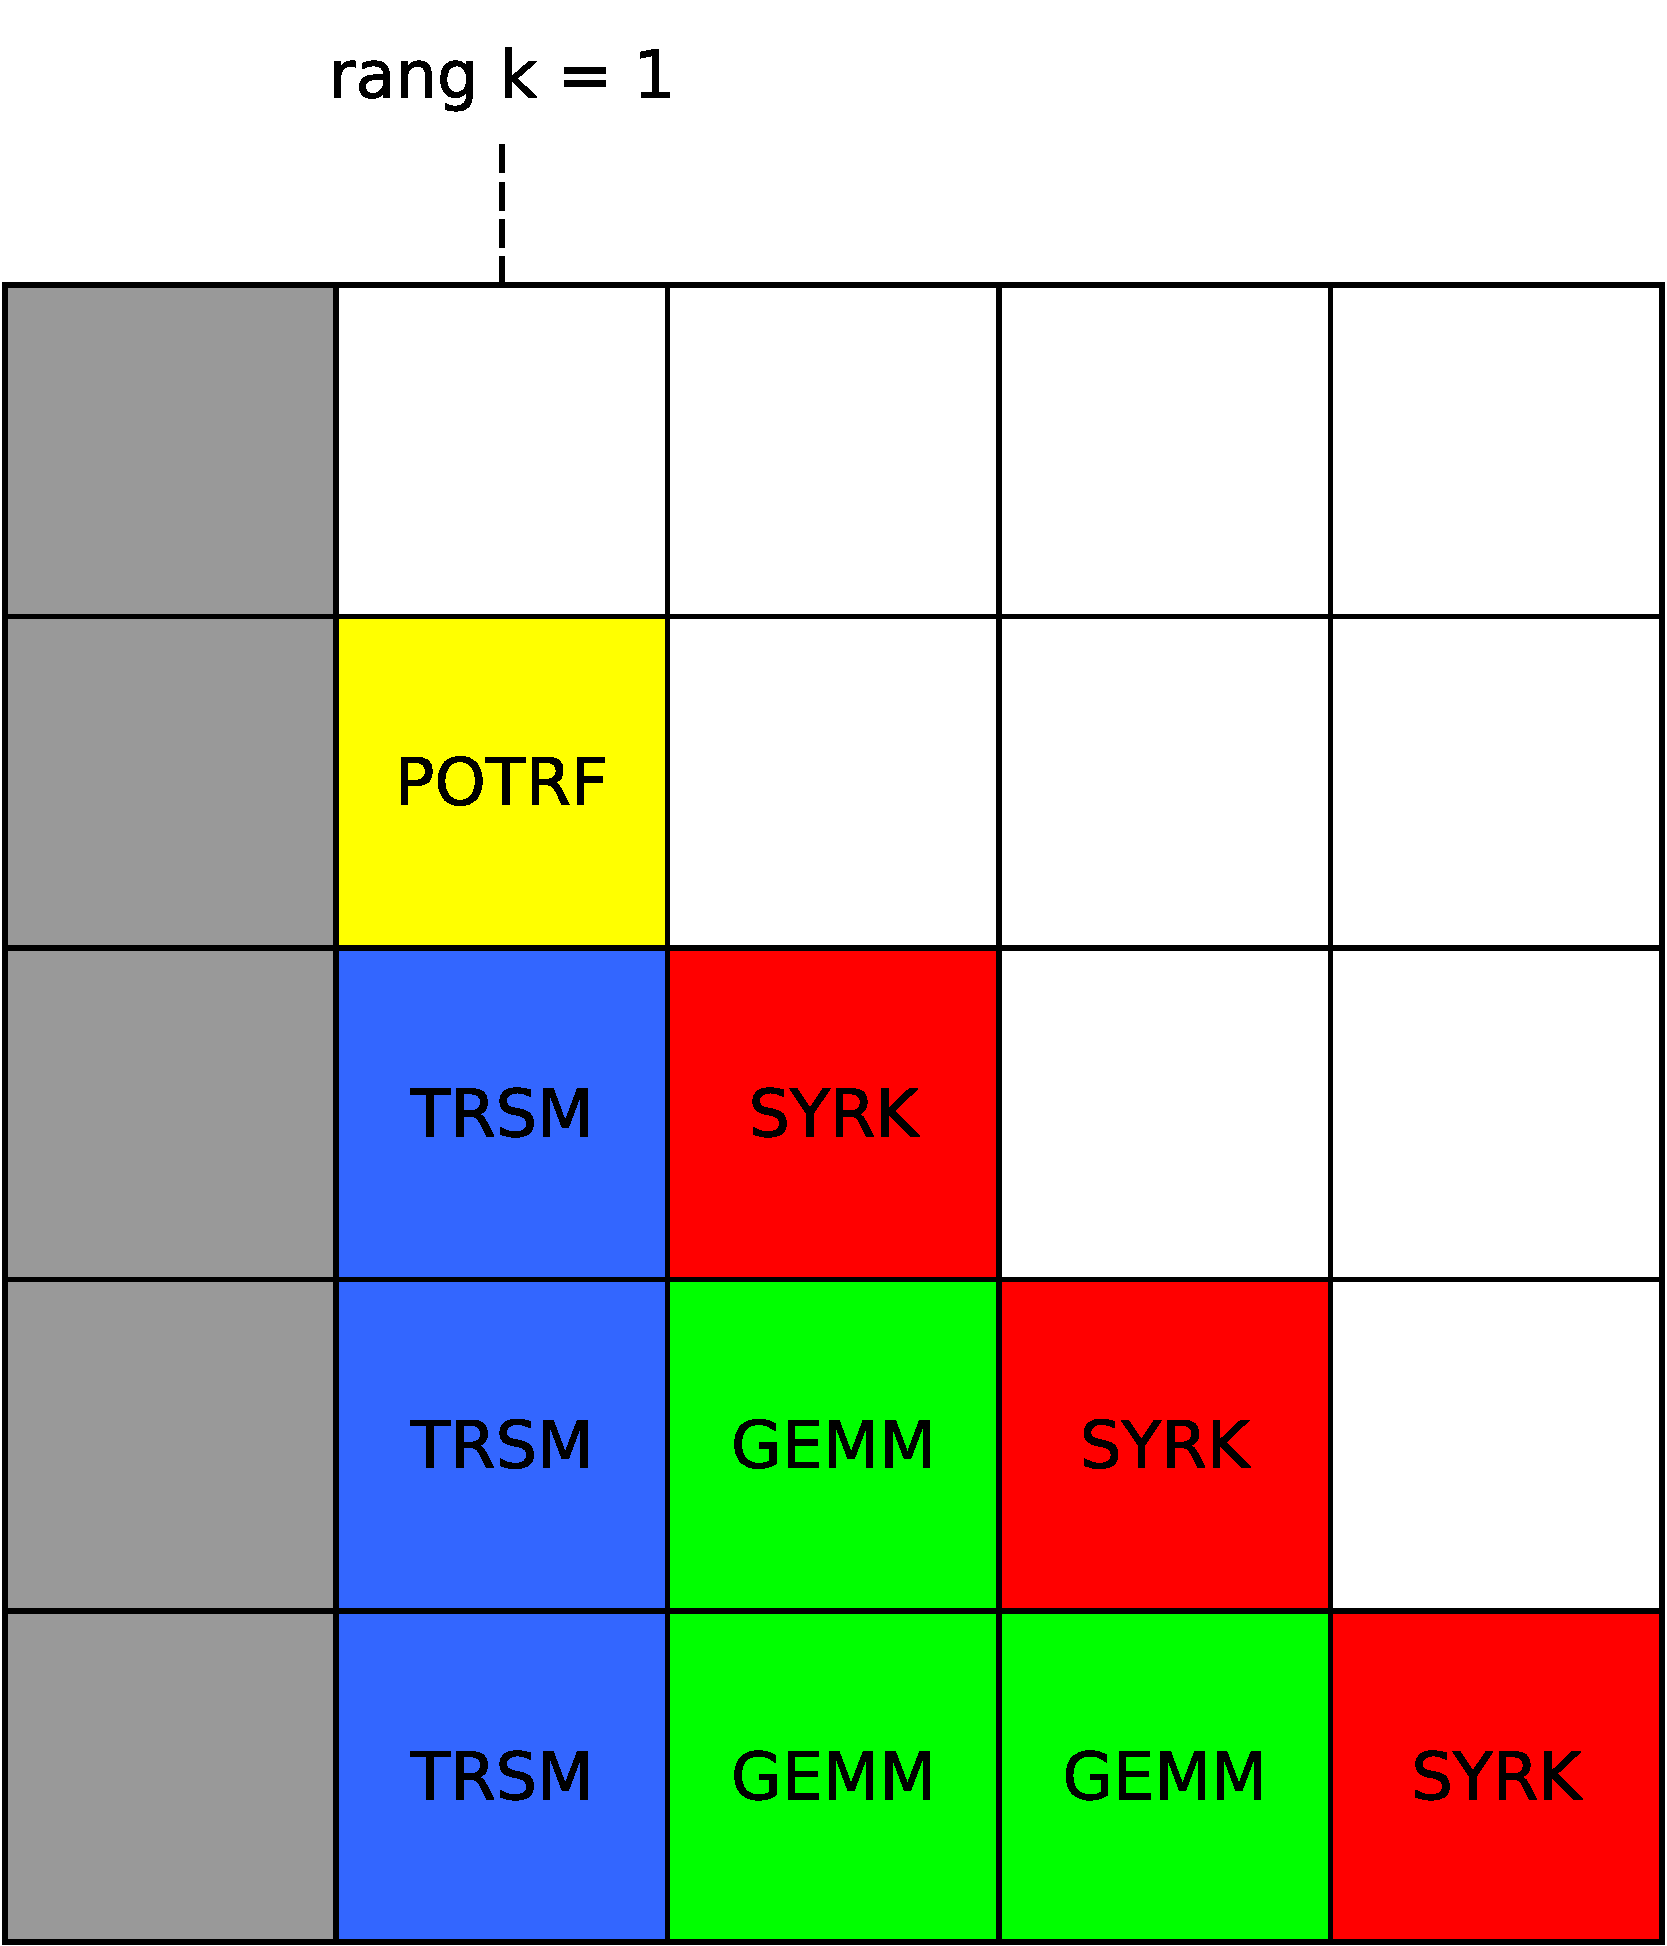
\includegraphics[width=0.6\textwidth]{cholesky-rank-update}
  \caption{Itération du rang k de la factorisation de Cholesky}\label{fig:contribs:apps:cholesky:rank-update}
\end{figure}

Pour permettre de mieux représenter l'algorithme du listing~\ref{lst:contribs:apps:cholesky-block-plasma}, les opérations se produisant sur chaque bloc de la matrice au rang |k| sont illustrées sur la figure~\ref{fig:contribs:apps:cholesky:rank-update}


À chaque itération, un \potrf est d'abord effectué sur le bloc diagonal de l'itération. Les blocs de la colonne sont ensuite mis à jour via des \trsm, à la suite desquels les autres blocs restant peuvent être mis à jour par des \gemm (ou \syrk pour les blocs diagonaux).
Le parallélisme de l'algorithme est donc principalement libéré par les \potrf ainsi que les \trsm.
Cela peut être illustré par la Figure~\ref{fig:contribs:apps:cholesky:dag-5}, qui donne le graphe de dépendances d'une factorisation de Cholesky de largeur 5.

\begin{figure}[h]
  \centering
  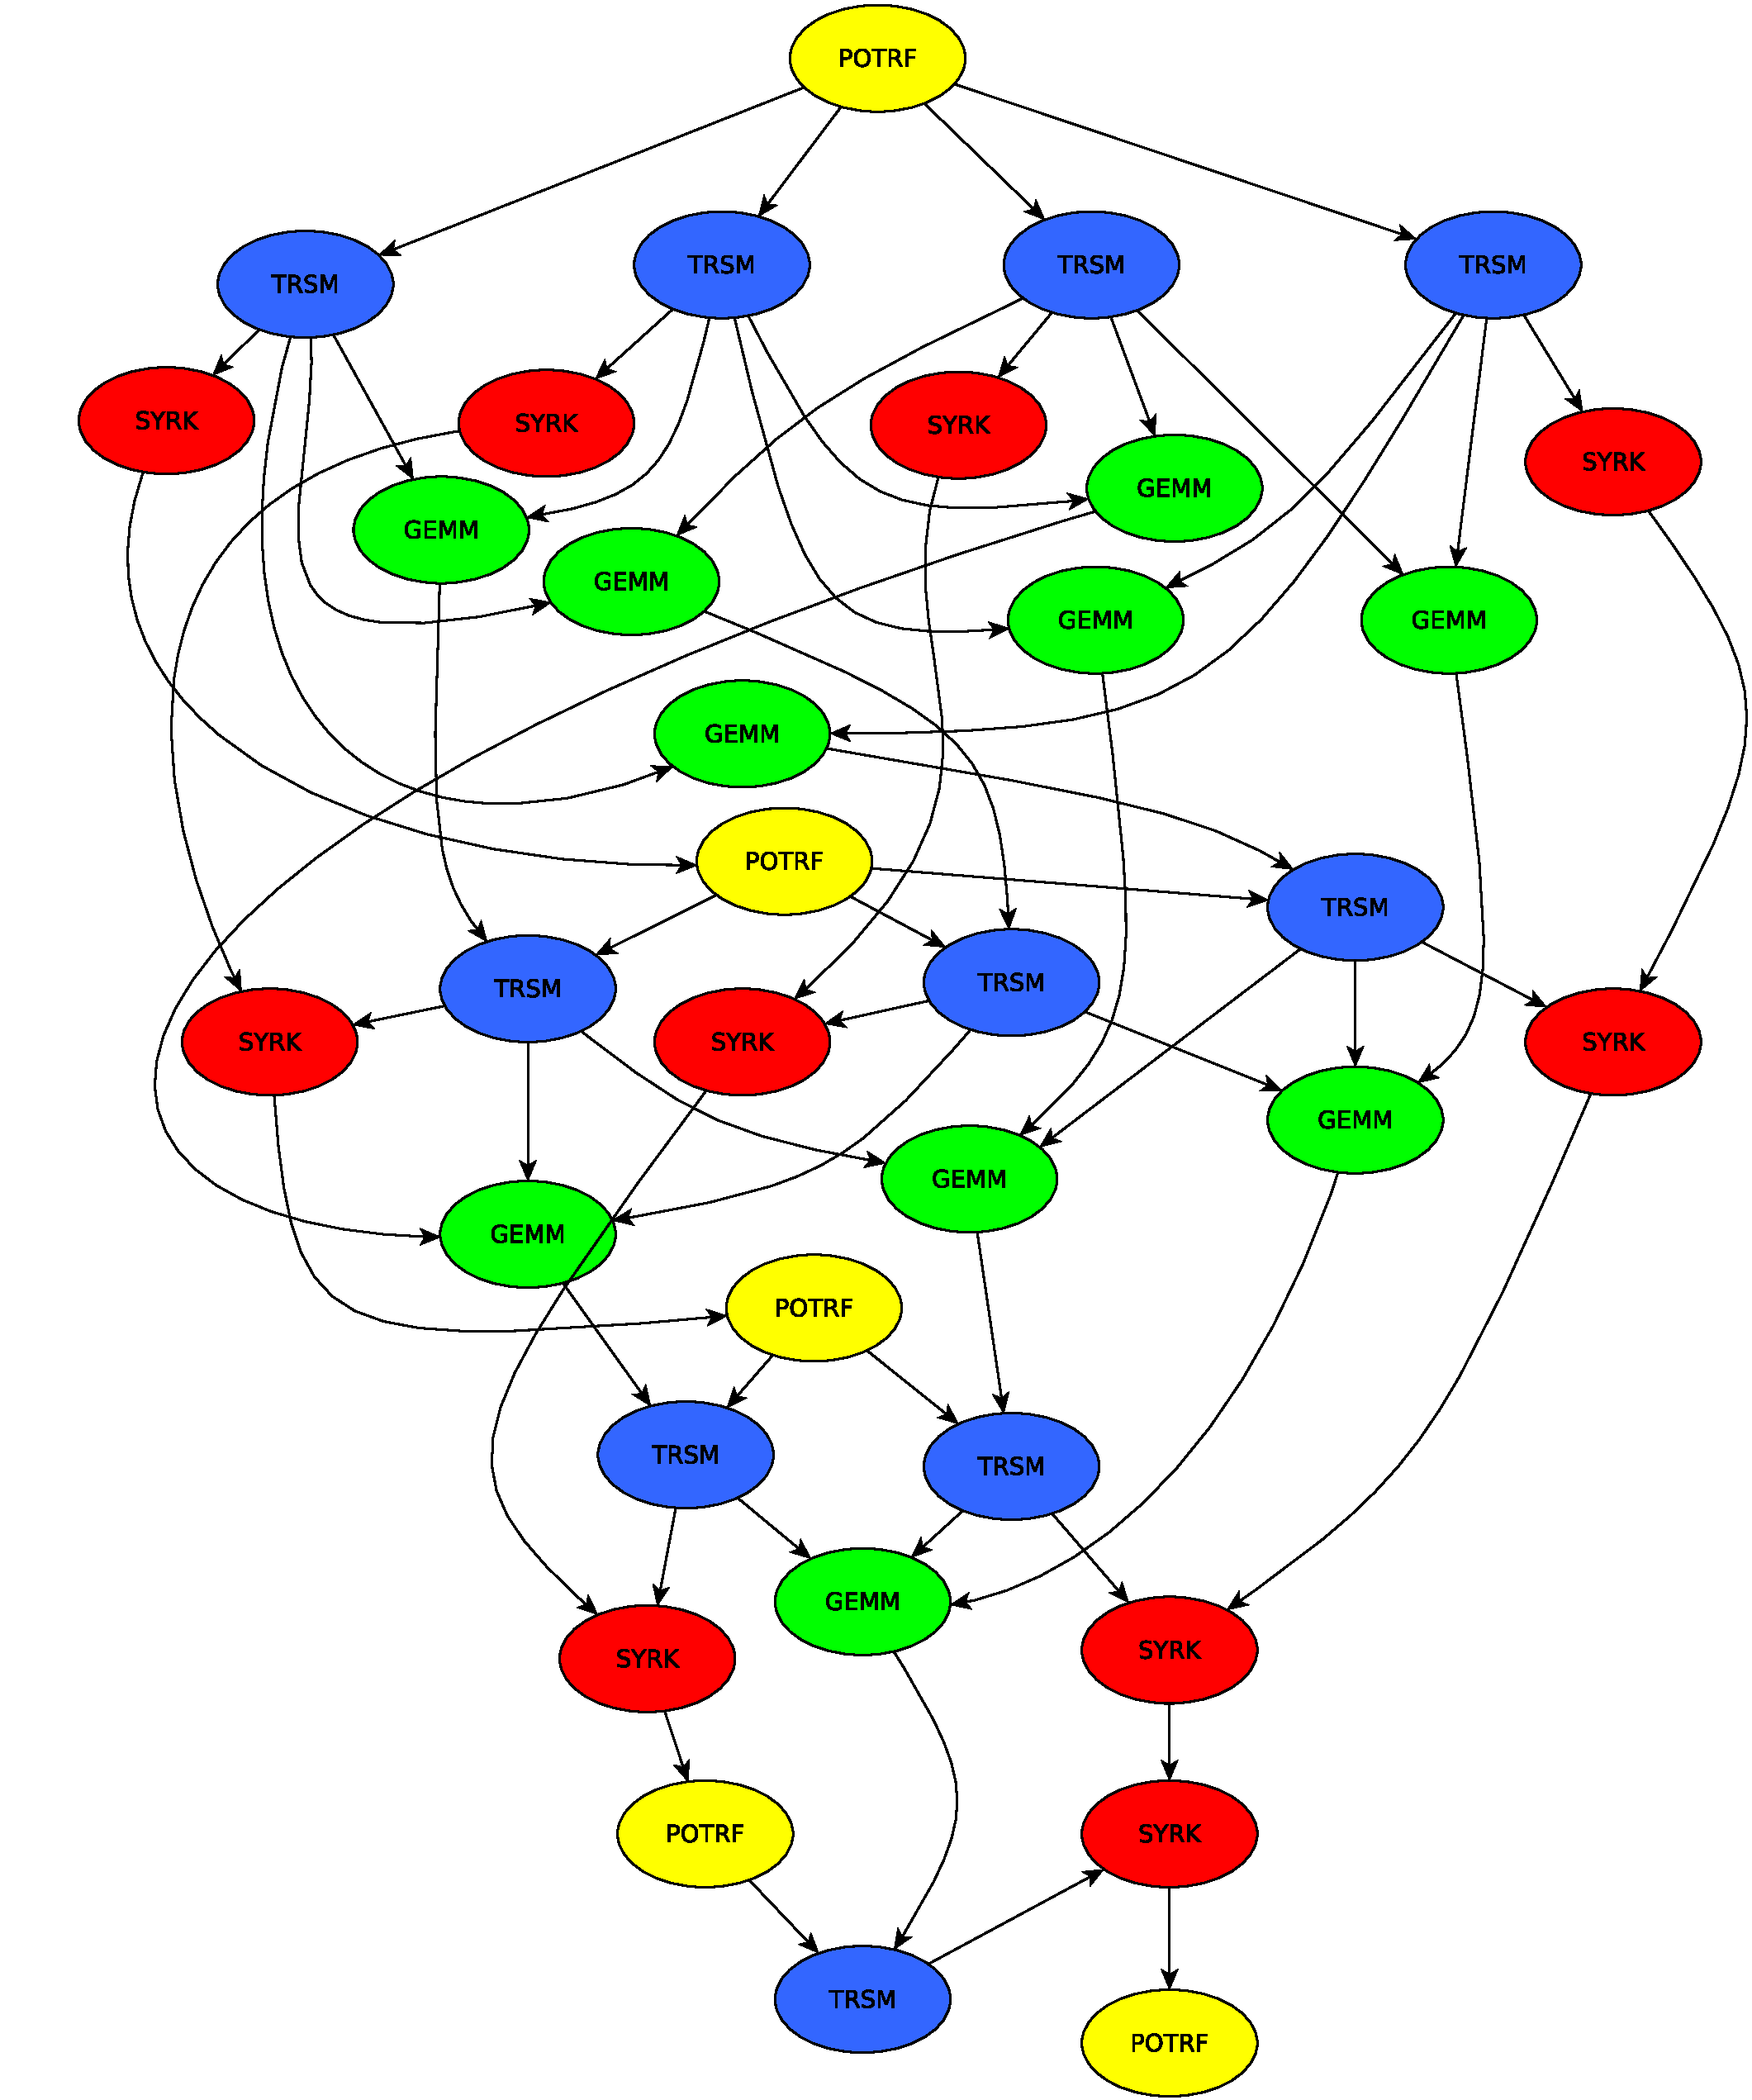
\includegraphics[width=0.7\textwidth]{cholesky-dag-5}
  \caption{DAG d'un Cholesky de largeur 5}\label{fig:contribs:apps:cholesky:dag-5}
\end{figure}

Le nombre de tâches créées pour une largeur de matrice $L$ (en nombre de blocs), le nombre d'opérations arithmétiques flottantes (ou \emph{flops}) en fonction de la taille de bloc $N$, ainsi que l'intensité opérationnelle\footnote{Définie par $\frac{Flops}{bytes}$} sont résumés dans la table~\ref{tab:contribs:apps:cholesky:kernels-info}.


\begin{table}[h!]
\def\arraystretch{1.5}
\centering
\begin{tabular}{|c||c|c|c|}\hline
  Noyau & \makecell{Nombre pour une\\largeur de matrice $L$} & \makecell{Flops pour une\\ taille de bloc $N$~\cite{LAWN41}} & \makecell{Intensité\\Opérationnelle} \\ \hline
  \potrf & $L$ & $\frac{N^3}{3} + \frac{N^2}{2} + \frac{N}{6}$ & $\frac{N}{24} + o(N)$ \\ \hline
  \trsm & $\frac{L*(L-1)}{2}$ & $N^3$ & $\frac{N}{8} + o(N)$ \\ \hline
  \syrk & $\frac{L*(L-1)}{2}$ & $N^2*(N+1)$ & $\frac{N}{8} +o(N)$ \\ \hline
  \gemm & $\frac{L^3}{6} - \frac{L^2}{2} + \frac{L}{3} + 1$ & $2*N^3$ & $\frac{N}{4} +o(N)$ \\ \hline
%$\sum_{k=1}^{n}\frac{(k-1)*(k-2)}{2}$
%simplifié via wolframalpha
\end{tabular}
\caption{Nombre et complexité des différents noyaux}\label{tab:contribs:apps:cholesky:kernels-info}
\end{table}

Les \gemm sont donc très largement majoritaires dans l'algorithme quand la largeur de la matrice augmente.
En revanche en terme de Flops et d'intensité opérationnelle, on peut constater que tous les noyaux présentent des chiffres d'un ordre de grandeur équivalent.


\subsection{Observations préliminaires et limites}\label{sec:contribs:apps:cholesky:observations}

Cette section et les suivantes montrent des évaluations reposant sur une bibliothèque BLAS, sauf indication contraire, la version utilisée est OpenBLAS 2.19.
La figure~\ref{fig:context:granularity} a montré qu'on pouvait observer l'impact de certains paramètres, tels que la taille de bloc ou le support exécutif, sur les performances globales.

Certains supports exécutifs tels que Kaapi, StarPU, OpenStream, ou encore OmpSs permettent d'aller plus loin via un système de traces, permettant d'observer certaines caractéristiques de tâches particulières.

\begin{figure}[t!]
  \centering
  \includegraphics[width=\textwidth]{graph_evolution_cholesky_8192_224}
  \caption{Évolution des performances de Cholesky avec libKOMP, pour une taille de matrice de 8192 et une taille de bloc de 224}\label{fig:contribs:apps:cholesky:overview-8192-224}
\end{figure}

Pour illustrer cela, prenons un exemple d'évolution des performances de Cholesky en fonction du nombre de cœurs utilisés, montré sur la figure~\ref{fig:contribs:apps:cholesky:overview-8192-224}. Dans cet exemple la taille de matrice est de 8192, la taille de bloc de 224, et le support exécutif utilisé est libKOMP, sans aucune extension relatives à nos travaux sur l'affinité des données, que nous présentons dans le chapitre~\ref{chap:contrib:openmp}.

En activant le support des traces, on peut avoir plus de détails sur l'exécution individuelle de chacune des tâches.

\begin{figure}[h!]
  \centering
  \includegraphics[width=\textwidth]{graph_distrib_overview_8192_224}
  \caption{Distribution des différents noyaux en fonction du nombre de cœurs}\label{fig:contribs:apps:cholesky:distrib-overview-8192-224}
\end{figure}

La figure~\ref{fig:contribs:apps:cholesky:distrib-overview-8192-224} montre, pour chaque type de tâche (ou \emph{noyau}), la répartition du temps d'exécution (en cycles) en fonction du nombre de cœurs.

On constate deux types de répartitions~:
\begin{itemize}
  \item Une distribution relativement restreinte des cycles de chaque noyau, typiquement observée pour 16 cœurs.
    La distribution peut avoir plusieurs pics~: pour \gemm sur 16 cœurs par exemple.
    Cela pourrait être expliqué par le nombre de cas possibles pour le placement des blocs de données manipulés par le noyau~: avec 16 cœurs il y a 2 nœuds impliqués, et donc 4 cas pour la position des blocs (3 locaux, 2 locaux, 1 local, 3 distants), ce qui pourrait correspondre aux 4 niveaux de performances observés.
  \item Une distribution relativement large, typiquement observée pour un grand nombre de cœur. Pour un \gemm sur 192 cœurs, le nombre de cycles nécessaires pour l'exécution peut varier du simple au double !
\end{itemize}

Nous souhaiterions identifier d'où vient cette évolution dans la distribution, afin d'éventuellement réussir à la corriger en limitant sa largeur.

Malheureusement il n'existait pas, à notre connaissance, d'outil permettant d'isoler une (ou plusieurs) tâches d'une application, et permettant de changer certains paramètres prédéfinis pouvant avoir un impact sur le temps d'exécution de la tâche.
Nous avons donc utilisé \outil dans le but de comprendre et d'analyser plus en profondeur nos observations préliminaires.

\subsection{Caractérisation détaillée des noyaux via \outil}\label{sec:contribs:apps:cholesky:carton}

L'objectif de cette section est de décrire le processus expérimental nous ayant permis d'analyser et comprendre le comportement des quatre noyaux de Cholesky~: \potrf, \trsm, \syrk, \gemm, qui a finalement abouti à des améliorations du support exécutif.
Nous allons donc aborder d'une part les types de scénarios exécutés via \outil, puis illustrer les résultats que nous avons obtenus avec des exemples significatifs.

\subsubsection{Description des scénarios}\label{sec:contribs:apps:cholesky:scenario}

Afin d'étudier le comportement de chaque noyau impliqué dans Cholesky, nous avons défini des scénarios au cours desquels les noyaux sont exécutés avec un contrôle sur les conditions d'exécution.

Pour un noyau donné (parmi \potrf, \trsm, \syrk, \gemm), le scénario de base est le suivant :
\begin{itemize}
  \item Allocation et initialisation des données sur un nœud précis pour une taille de bloc donnée.
  \item Exécution d'un certain nombre de répétitions du noyau choisi (par défaut 50) sur ces données, en plaçant le thread de calcul soit sur un cœur du même nœud que les données, soit sur un cœur distant.
  \item Observation de la performance en FLOPS.
\end{itemize}

Ce scénario de base est donné en entier dans l'annexe~\ref{chap:annexe:tool:dgemm-base}, pour l'exécution d'un \gemm local de taille 256.

Pour évaluer le comportement des noyaux en fonction de la charge de la machine, nous avons créé des scénarios exécutant simultanément plusieurs noyaux sur des données complètement indépendantes, et où le démarrage de l'exécution des noyaux est synchronisé.
L'annexe~\ref{chap:annexe:tool:dgemm} illustre l'un de ces scénarios, qui permet d'exécuter 8 \gemm en parallèle, sur des données locales complètement indépendantes, avec une taille de matrice de 256.

Il y a plusieurs paramètres que l'on peut faire varier pour changer les conditions d'exécution~:
\begin{itemize}
  \item Le nombre de noyaux s'exécutant simultanément~;
  \item L'utilisation de données distantes ou locales~;
  \item La taille du bloc sur lequel appliquer le noyau.
\end{itemize}

Les trois sections suivantes décrivent l'impact des changements de ces paramètres, et illustrent certaines caractéristiques des machines utilisées qui donnent des opportunités pour de possibles améliorations du support exécutif.

\subsubsection{Exécutions simultanées}

\begin{figure}[ht]
  \centering
  \includegraphics[width=0.95\textwidth]{kernel_256_local_idchire}
  \caption{Performances des noyaux (B=256) avec données locales sur idchire}\label{fig:contribs:apps:cholesky:perf-256-local}
\end{figure}

Afin d'évaluer l'impact de la charge de la machine, nous avons lancé des scénarios avec un nombre variable d'exécutions simultanées de chacun des noyaux.
Pour le remplissage de la machine, nous avons placé les exécutions linéairement sur la machine, remplissant progressivement un nœud après l'autre.

La figure~\ref{fig:contribs:apps:cholesky:perf-256-local} montre la performance moyenne (en GFlops) de chaque noyau, en fonction du nombre de cœurs exécutant simultanément des noyaux.
Par exemple pour déterminer le point d'abscisse 144 sur la figure pour un \gemm, nous avons exécuté 50 répétitions de \gemm sur chacun des 144 premiers cœurs de la machine idchire (remplissant donc les 18 premiers nœuds), de manière indépendante et simultanée.
La performance moyenne pour ce point est obtenue en faisant la moyenne des performances sur l'ensemble des exécutions.
Pour ce cas la taille de bloc a été fixée à 256, avec les données allouées et initialisées localement.

Pour une taille de bloc de 256, la quantité maximale de données utilisée par l'un des noyaux (\gemm) est de 256*256*8*3 = 1.5 Mo. La taille du cache L2 étant de 256 Ko, le jeu de données ne tient pas dans ce cache. Mais avec un nœud de 8 cœurs exécutant 8 exécutions concurrentes, la quantité totale de données utilisée serait au pire de 12.58 Mo, soit environ 50\% des 20Mo de cache L3 disponible.
On pourrait donc s'attendre à ce que la performance moyenne des noyaux ne soit impactée que par des effets locaux aux nœuds.

Néanmoins les courbes montrent clairement une dégradation des performances de chaque noyaux lorsque la charge de la machine augmente.
Ce comportement a également été observé pour d'autres tailles de blocs. Sur brunch le comportement a été également observé, avec néanmoins une dégradation moindre.

\begin{todo}
  faire la mesure via hubstat pour confirmer ou infirmer l'hypothèse de la cohérence.

  %https://www.researchgate.net/profile/Daniel_Molka/publication/315703632_Performance_Analysis_of_Complex_Shared_Memory_Systems/links/58dd3cf292851cd2d3d9d5d3/Performance-Analysis-of-Complex-Shared-Memory-Systems.pdf
  %https://pdfs.semanticscholar.org/67cf/1189c859d66bac309f9438df434fb651f97a.pdf
  % sandy bridge : https://tu-dresden.de/zih/forschung/ressourcen/dateien/abgeschlossene-projekte/benchit/2014_MSPC_authors_version.pdf?lang=en
  % haswell : https://pdfs.semanticscholar.org/67cf/1189c859d66bac309f9438df434fb651f97a.pdf
\end{todo}

\subsubsection{Impact de la localité des accès}\label{sec:contribs:apps:cholesky:locality}

Les expériences de bande passante dans la section précédente ont montrées des différences significatives dans les temps d'accès à la mémoire locale et distante.
Nous avons donc déroulé des scénarios avec des noyaux utilisant des données distantes ou des données locales afin de pouvoir les comparer, et éventuellement déceler des comportements typiques.
Lorsque les données sont dites <<locales>>, l'ensemble des données est allouée sur le nœud local. Lorsque les données sont dites <<distantes>>, l'ensemble des données est alloué sur le nœud suivant (numériquement) dans la hiérarchie de la machine.

\begin{figure}[t!]
  \centering
  \includegraphics[width=0.95\textwidth]{kernel_512_remote_idchire}
  \caption{Performances GEMM, POTRF (B=512) avec données distantes sur \emph{idchire}}\label{fig:contribs:apps:cholesky:perf-512-remote-idchire}
\end{figure}
\begin{figure}[h!]
  \centering
  \includegraphics[width=0.95\textwidth]{kernel_512_remote_brunch}
  \caption{Performances GEMM, POTRF (B=512) avec données distantes sur \emph{brunch}}\label{fig:contribs:apps:cholesky:perf-512-remote-brunch}
\end{figure}

Les figures~\ref{fig:contribs:apps:cholesky:perf-512-remote-idchire} et~\ref{fig:contribs:apps:cholesky:perf-512-remote-brunch} illustrent les performances de deux noyaux, \gemm et \potrf, exécutés en concurrence sur des blocs de 512, en fonction du type d'accès, sur idchire et brunch, respectivement.

Avec une telle taille de bloc, l'ensemble des données pour tous les \potrf tient dans le cache L3, mais ce n'est pas le cas pour \gemm.
Pour les \potrf la dégradation de performances est moindre : les données tiennent dans le cache L3, il y a donc un coût pour rapatrier les données, mais une fois les données dans le cache L3 il n'y a plus besoin de faire d'accès distants.

Pour les \gemm, une utilisation de seulement quelques cœurs ne montre pas une différence de performances flagrante, en revanche le lien en sortie de nœud arrive assez vite à saturation (voir section~\ref{sec:contribs:machines:idchire:liens}), ce qui entraine une dégradation massive de performances.
À la fois pour idchire et brunch, on peut observer l'impact de la bande passante sur les performances~: les exécutions sont placées de manière à remplir progressivement les différents nœuds de la machine, et on peut observer que les courbes sont en dent de scie avec une période égale à la taille des nœuds sur chaque machine (8 sur idchire, 24 sur brunch).

Cela devient évident lorsqu'on regarde plus en détail le passage d'un nœud à un autre.
Sur la figure~\ref{fig:contribs:apps:cholesky:perf-512-remote-brunch}, la courbe pour les \gemm distants remonte progressivement entre 24 et 36 cœurs utilisés~: le fait de faire la moyenne des noyaux sur l'ensemble des cœurs cache légèrement le phénomène de saturation du lien.
En revanche ce phénomène devient évident lorsque l'on affiche la moyenne du temps d'exécution par cœurs pour certains des points de la courbe, comme illustré sur la figure~\ref{fig:contribs:apps:cholesky:distrib-load-512}.

\begin{figure}[ht]
  \centering
  \includegraphics[width=0.95\textwidth]{illustration_load_avg}
  \caption{Distribution des performances de chaque noyau (Bloc = 512), en fonction du nombre total d'exécutions concurrentes, sur brunch.}\label{fig:contribs:apps:cholesky:distrib-load-512}
\end{figure}

Le premier panneau montre la distribution des \gemm et des \potrf pour une exécution sur 24 cœurs concurrents situés sur le même nœud.
Cette distribution montre un unique pic bien défini pour chaque noyau (environ 12.5 GFlops pour \potrf, et 16.5 pour \gemm).
En revanche le passage à 26 cœurs (avec donc 2 cœurs situés seuls sur un autre nœud), montre une distribution avec deux pics~: un pic important correspondant au 24 premiers cœurs, et un second pic plus petit, montrant des performances beaucoup plus grandes, pour les 2 cœurs situé sur l'autre nœud.
Les autres panneaux montrent l'évolution de ces pics pour arriver au panneau 48, où les deux nœuds sont complètement utilisés.

%Note : Ici il y a aussi deux pics sur le panneau 48. Cela doit venir de la manière dont j'ai initialisé les accès distants : le premier nœud utilise des données du deuxième nœud, qui utilise des données du troisième nœud. Donc en pratique les liens du deuxième nœuds sont plus utilisés que ceux du premier : il doit donc un peu peiner à fournir les données nécessaires au premier nœud, ce qui expliquerait pourquoi il y a deux groupes de perf.


L'impact de la localité des données est majeur dans le cas où le jeu de données manipulé par l'ensemble des cœurs ne tient pas dans les caches L3.
Étant donné que la plus grande proportion des noyaux de Cholesky manipule 2 ou 3 blocs, la dégradation de performance devrait être importante lorsque la taille de bloc dépasse environ 320.

% Note : à la fois sur brunch et idchire, chaque cœur peut utiliser environ 2.5Mo de cache L3



\subsubsection{Impact de la taille de bloc}

La figure~\ref{fig:contribs:apps:cholesky:perf-multiple-bs-idchire} montre la performance des \gemm et \potrf sur idchire en fonction de la taille de bloc et du nombre de cœurs utilisés (tous les accès sont locaux).

\begin{figure}[ht]
  \centering
  \includegraphics[width=0.95\textwidth]{kernels_multiple_bs_local_idchire}
  \caption{Performances des noyaux avec données locales sur idchire}\label{fig:contribs:apps:cholesky:perf-multiple-bs-idchire}
\end{figure}

La taille de bloc n'a pas d'impact significatif sur le phénomène observé précédemment de dégradation des performances.
Elle a bien un impact sur le niveau de performance globale de chaque noyau (qui dépend de l'implémentation des BLAS), mais le comportement général de chaque noyau reste le même.

Cette conclusion est similaire lors d'un placement distant des données.


\subsubsection{Impact de la bibliothèque BLAS}

Pour comparer l'impact potentiel de la bibliothèque implémentant les BLAS, nous avons configuré \outil pour qu'il utilise soit OpenBLAS (2.19), Intel MKL (11.3), ou ATLAS (3.10.3).
La figure~\ref{fig:contribs:apps:cholesky:perf-blas} montre la performance des \gemm et \potrf sur \emph{brunch}, pour une taille de bloc de 256 avec des données locales, en fonction de la bibliothèque BLAS utilisée.

\begin{figure}[ht]
  \centering
  \includegraphics[width=0.98\textwidth]{comparaison_atlas_openblas_mkl_256_local}
  \caption{Comparaison des bibliothèques BLAS sur \emph{brunch}, données locales, taille de bloc = 256}\label{fig:contribs:apps:cholesky:perf-blas}
\end{figure}

Bien qu'on puisse constater une différence de performance brute, il y a dans tous les cas une baisse (relativement faible) des performances avec l'augmentation du nombre d'exécution concurrentes, bien qu'elles soient toutes indépendantes.
Pour rappel sur \emph{brunch} chaque nœud dispose de 24 cœurs, et pour les \gemm on peut deviner une baisse sur ces 24 premiers cœurs, qui d'autant plus flagrante que la performance est grande.
Cela pourrait tout simplement s'expliquer par le fait qu'on atteint la limite de bande passante cumulée disponible sur le nœud local.
Pour les autres cas, l'impact de la bibliothèque semble concerner principalement le pic de performance de chaque noyau, sans différence majeure sur l'allure générale des courbes.

\subsection{Bilan et discussions}

La figure~\ref{fig:contribs:apps:cholesky:distrib-overview-8192-224} avait montrée, à l'aide des traces obtenues à partir d'une exécution, que nous pouvions observer une baisse et une dispersion des performances individuelles des noyaux de l'application Cholesky.
\outil nous a permis d'identifier principalement deux facteurs pouvant être à l'origine de ce phénomène~: tout d'abord une partie de la baisse de performance générale est due à la baisse de performance des noyaux qui accompagne l'augmentation de la charge de la machine.
\begin{todo}
  rappeler d'où ça vient quand c'est fait
\end{todo}
L'autre partie de cette baisse de performance, ainsi que la dispersion des temps d'exécution, peuvent être attribuées à une absence de contrôle de la localité des données au cours de l'application.



\bigskip
\bigskip

\tool nous a permis de mettre en évidence certaines caractéristiques des machines et des parties critiques d'une application utilisée comme étude de cas.
Le chapitre suivant est axé sur les différentes extensions que nous avons proposées dans le modèle de programmation et le support exécutif, afin d'essayer de mitiger le manque de localité des données.
En pratique les observations faites à travers \outil nous ont également servies à sélectionner des expériences et paramètres pertinents lors de l'évaluation des stratégies de vol de travail proposées avec la factorisation de Cholesky.


%\begin{savequote}[6cm]
%<< truc
%\qauthor{Test}
%\end{savequote}

\chapter{Utilisation et amélioration d'OpenMP}\label{chap:contrib:openmp}
\chaptertoc


%\input{tex/OpenMP on numa}
% Big section to describe how we use/extend OpenMP to exploit these architectures

% - Description of OpenMP language (tasking and such)
% - Description of OpenMP runtime

% - Motivating examples for our works using current OpenMP

% - Missing to improve things
%    - What we implemented
%    - What remains

Ce chapitre regroupe les différentes contributions que nous avons faites spécifiquement dans le contexte d'OpenMP.
Cela inclu tout d'abord une suite de benchmarks, KASTORS, regroupant un ensemble de programmes implémentés à l'aide des tâches avec dépendances d'OpenMP, et décrite dans la section~\ref{sec:openmp:kastors}.
Nous décrivons ensuite des extensions dédiées à l'amélioration de la localité des données dans la section~\ref{sec:openmp:langage}.
La section~\ref{sec:openmp:runtime} aborde les modifications faites au niveau du support exécutif pour qu'il puisse avoir une vision hiérarchique de la machine, et qu'il puisse exploiter les informations fournies par les extensions du langage OpenMP proposées.
Enfin toutes ces propositions sont évaluées dans la section~\ref{sec:contribs:perf_eval}.

\section{Préambule : une suite de benchmarks pour OpenMP~4.0, les KASTORS}

\subsection{Motivation pour une nouvelle suite de benchmarks}

Le support pour les applications à base de flots de données dans OpenMP est arrivé avec la version 4.0, qui est sortie au démarrage de cette thèse.
Nous n'avions donc pas d'applications de référence pour utiliser les fonctionnalités ajoutées dans OpenMP, et nous avons donc décidé d'introduire une suite de benchmarks - les KASTORS~\cite{Virouleau2014} - spécifiquement orientée vers ces fonctionnalités, en étendant et regroupant certaines applications existantes.

Il existe évidemment plusieurs suites de benchmarks à destination des architectures à mémoire partagée : d'une part pour les applications à base de tâches indépendantes et utilisant OpenMP~3.0, et d'autre part pour les applications à base de flots de données, mais écrites dans des langages différents.

Parmi les benchmarks populaire ciblant spécifiquement OpenMP, on peut citer la Barcelona OpenMP Task Suite~\cite{Duran2009} (BOTS), proposant des applications à base de tâches OpenMP~3.0 afin d'évaluer le comportement d'OpenMP en fonction de la manière de générer les tâches et de la répartition de la charge de travail.
Nous avons d'ailleurs adapté certaines de leurs applications - SparseLU et Strassen - dans les KASTORS, dont nous parlons plus en détails dans les sections~\ref{sec:kastors:sparselu} et~\ref{sec:kastors:strassen}

Parmi les benchmarks ciblant des modèles de programmations à base de tâche avec dépendances, on peut principalement nommer les PLASMA~\cite{Kurzak2013}.
Cette bibliothèque développée à ICL/UTK met à disposition un grand nombre d'algorithmes d'algèbre linéaire dense, optimisés pour les architectures multi-coeurs.

Nous avions donc assez d'éléments de base pour construire un ensemble d'applications, avec en tête les objectifs suivant :
\begin{itemize}
  \item Rassembler et proposer une suite d'applications exploitant les dépendances introduites avec OpenMP~4.0
  \item Comparer la version utilisant des flots de données à la version utilisant des synchronisations explicites. Le but étant de montrer que le support exécutif peut gérer les synchronisations plus finement, et par conséquent améliorer les performances sans changer l'algorithme.
  \item Avoir une base adaptée pour développer les extensions présentées dans les sections~\ref{sec:openmp:langage} et~\ref{sec:openmp:runtime}.
\end{itemize}

Les sections suivantes décrivent les différents applications de la suite : d'où ils viennent, comment nous les avons étendu pour utiliser les dépendances de données, ainsi que comment nous les avons intégrés.


\subsection{Description des applications}

Les applications suivantes proviennent de différentes suites de benchmarks, et ont été modifiées afin d'utiliser les dépendances de données plutôt que d'autres moyen de synchronisation.

\subsubsection{Factorisations de Cholesky, QR, et LU}

Ces trois applications ont été adaptées des PLASMA.
Dans les PLASMA plusieurs implémentations de chaque algorithme sont disponibles, utilisant soit un ordonnancement statique, soit un ordonnancement dynamique.
Les algorithmes à ordonnancement dynamique sont construit sur le support exécutif QUARK~\cite{YarKhan2011}, qui utilise un modèle avec dépendances de données pour ordonnancer les tâches.

Les trois algorithmes que nous avons sélectionné sont les factorisations de Cholesky, QR, et LU, respectivement nommés DPOTRF, DGEQRF, et DGETRF dans PLASMA.
Ils opèrent tous sur des matrices de nombres flottant à double précision (type |double|).

L'implémentation initiale utilise plusieurs niveaux de wrappers, avec packing et unpacking de paramètres à chaque niveau, ce qui affecte la lisibilité du code et augmente grandement le risque d'erreur.

Les listings~\ref{lst:kastors:dyn} et~\ref{lst:kastors:dyn-omp} montrent respectivement la version dynamique originale, et les transformation que l'on a fait pour porter le code en OpenMP~4.0.
Dans la version originale, la function |wrapper_blas_function| effectue l'unpacking des paramètres avant d'appeler la vraie fonction BLAS/LAPACK sur laquelle elle est construite.
La transformation en OpenMP~4.0 a donné lieu au retrait de plusieurs niveau d'encapsulation, ce qui facilite la lecture du code, la maintenabilité du code, et enlève le besoin de gérer ces paramètres.

\begin{lstlisting}[caption=Format de l'algorithme dynamique,label=lst:kastors:dyn]
wrapper_algorithm_dynamic_call(...) {
  // code séquentiel
  for (...)
    QUARK_Insert_Task(wrapper_blas_function, packed_parameters);
  // code séquentiel
  for (...)
    QUARK_Insert_Task(
        wrapper_another_blas_function,
        packed_parameters);
  // code sequentiel
}
\end{lstlisting}
\begin{lstlisting}[caption=Format de l'algorithme OpenMP,label=lst:kastors:dyn-omp]
algorithm_call(...) {
    // code séquentiel
    for (...)
#pragma omp task depend(inout:array[...])
        blas_function(...);
    // code séquentiel
    for (...)
#pragma omp task depend(inout:array[...])
        another_blas_function(...);
    // code séquentiel
}
\end{lstlisting}


\subsubsection{Jacobi}

C'est un algorithme de type Stencil : c'est un algorithme itératif, et à chaque itérations les différents éléments d'un tableau sont mis à jour en suivant la même formules dépendant généralement des éléments voisins.

En pratique cet algorithme résout l'équation de Poisson sur le carré unitaire [0,1]x[0,1], qui est divisé en une grille de NxN points espacés régulièrement.
Le noyau de calcul principal est un Stencil à 5 points, en 2 dimensions.
Ce noyau est appliqué successivement jusqu'à ce qu'une convergence soit détectée.

Nous avons implémenté deux versions bloquées de ce noyau, en utilisant d'une part des tâches sans dépendances, et d'autre part des tâches avec dépendances.

\subsubsection{SparseLU}\label{sec:kastors:sparselu}

Cette application calcule la factorisation LU d'une matrice creuse.
Nous avons modifié l'implémentation originale des BOTS pour ajouter des dépendances de données.
Ces modifications sont décrites dans les listings~\ref{lst:kastors:sparseLU} et~\ref{lst:kastors:sparseLU-deps}.

\begin{lstlisting}[caption=LU utilisant des tâches indépendantes,label=lst:kastors:sparseLU]
for (k=0; k<NB; k++) {
  lu0(M[k*NB+k]);
  for (j=k+1; j<NB; j++)
#pragma omp task untied shared(M)
    fwd(M[k*NB+k], M[k*NB+j]);

  for (i=k+1; i<NB; i++)
#pragma omp task untied shared(M)
    bdiv(M[k*NB+k], M[i*NB+k]);

#pragma omp taskwait

  for (i=k+1; i<NB; i++)
    for (j=k+1; j<NB; j++)
#pragma omp task untied shared(M)
      bmod(M[i*NB+k],
           M[k*NB+j],
           M[i*NB+j]);
#pragma omp taskwait
}
\end{lstlisting}

\begin{lstlisting}[caption=LU utilisant des tâches avec dépendances,label=lst:kastors:sparseLU-deps]
for (k=0; k<NB; k++) {
#pragma omp task untied shared(M)\
    depend(inout: M[k*NB+k:BS*BS])
  lu0(M[k*NB+k]);
  for (j=k+1; j<NB; j++)
#pragma omp task untied shared(M)\
    depend(in: M[k*NB+k:BS*BS])\
    depend(inout: M[k*NB+j:BS*BS])
    fwd(M[k*NB+k], M[k*NB+j]);

  for (i=k+1; i<NB; i++)
#pragma omp task untied shared(M)\
    depend(in: M[k*NB+k:BS*BS])\
    depend(inout: M[i*NB+k:BS*BS])
    bdiv(M[k*NB+k], M[i*NB+k]);

  for (i=k+1; i<NB; i++)
    for (j=k+1; j<NB; j++)
#pragma omp task untied shared(M)\
   depend(in: M[i*NB+k:BS*BS])\
   depend(in: M[k*NB+j:BS*BS])\
   depend(inout: M[i*NB+j:BS*BS])
    bmod(M[i*NB+k],M[k*NB+j],M[i*NB+j]);
}
\end{lstlisting}

\subsubsection{Strassen}\label{sec:kastors:strassen}

L'application Strassen utilise des décompositions de matrices pour calculer le produit de grandes matrices denses.
De manière similaire à SparseLU, nous avons modifié l'implémentation des BOTS pour ajouter du parallélisme au niveau des additions dans l'algorithme, et nous avons exprimé des dépendances de données plutôt que d'utiliser une synchronisation à base de |taskwait|.

\subsection{Discussions et perspectives}

Nous avons évalué l'intérêt des tâches avec dépendances comparé aux tâches indépendantes dans l'article publié à IWOMP2014~\cite{Virouleau2014}.
Les expériences ont été mené sur toutes les applications avec plusieurs supports exécutifs.
Les résultats ont montrés que l'utilisation des dépendances n'était jamais négatif pour les performances, et induisait en fait une amélioration dans la majorité des cas que nous avons testé.
Cela a pu confirmer que les supports exécutifs pouvaient gérer les synchronisations finement, éliminant ainsi les inactivités des threads dues aux |taskwait|.

D'autres part, ces applications et expériences ont permises de mettre en évidence d'autres limitations des tâches OpenMP.

\begin{figure}[ht]
  \centering
  \includegraphics[width=\textwidth]{jacobi_scale_noaff}
  \caption{Comparaison des performances de Jacobi sur idchire, avec une taille de matrice de 49152}\label{fig:contribs:openmp:kastors:jacobi-motiv}
\end{figure}

La figure~\ref{fig:contribs:openmp:kastors:jacobi-motiv} regroupe une comparaison de l'application de jacobi en fonction de la version implémentée (à base de boucles ou de tâche avec dépendances) et du support exécutif, effectuée sur idchire.
La scalabilité de l'application en elle même est limitée, mais il n'y a pas de raison, a priori, qu'il y ait une dégradation de performances de l'application avec l'augmentation du nombre de cœurs.
Jacobi est une application stencil, et chacune des tâches successives (ou groupe d'itérations pour la version à base de boucles) dépend énormément de la réutilisation du cache L2~: la structure de tâches ne permet pas d'exprimer ce genre de <<dépendances>>, lors de l'ordonnancement certaines tâches vont se faire voler et briser la localité du cache L2, introduisant une grosse dégradation des performances.

Ce problème pourrait être résolu si l'on pouvait exprimer une \emph{affinité} entre une tâche et un cœur de la machine, par exemple.
De plus les résultats de la section~\ref{sec:contribs:apps:cholesky:carton} ont montrés l'importance de la proximité des données pour les différents noyaux de Cholesky, ce qui représente une autre motivation pour la proposition d'une clause permettant l'expression d'une \emph{affinité} entre une tâche et un élément de la machine.

La section suivante aborde ce point, et la section~\ref{sec:contribs:perf_eval} décrit les résultats obtenus à partir des KASTORS étendus avec nos propositions.


\section{Amélioration de l'expressivité du langage}\label{sec:openmp:langage}

Nous avons proposé plusieurs extensions au langage et à l'API d'OpenMP, dont le but général est de faciliter le travail du support exécutif pour maintenir la proximité entre une tâche et ses données au cours de l'exécution du programme.

\subsection{Description du besoin}

Dans un contexte où l'on souhaite améliorer le contrôle sur les tâches et leurs données, OpenMP~4.0 ne propose que deux fonctionnalités~: les |OMP_PLACES| et |OMP_PROCBIND|, mais cela n'a d'effet que sur le placement des threads sur la topologie, et non sur les tâches qui leur sont attribuées.
Il n'y a rien au sein d'OpenMP qui permet d'exprimer une relation entre une tâche et une donnée ou une partie de la topologie de la machine.

En dehors d'OpenMP, les programmeurs utilisent généralement des bibliothèques ou outils externes dans le but de contrôler le placement des données, tels que MAi~\cite{Pousa2009} et MaMi~\cite{Broquedis2010a}.
L'efficacité de certaines approches peut être remise en cause (comme dans le cas de \emph{numactl}), et les approches utilisant une bibliothèque externe peuvent être relativement intrusives.

Nous avons donc introduit deux types de constructions dans OpenMP~: d'une part un moyen de contrôler la distribution initiale des données manipulées par les tâches, et d'autres part un moyen d'associer les tâches à ces données (ou mieux, à n'importe quelle partie de la machine).

\subsection{Contrôle de la distribution des données}\label{sec:openmp:langage:init}

Utiliser une initialisation séquentielle des données de son application peut avoir des conséquences dramatiques sur les performances, tout spécialement lorsque l'on cible des machines NUMA.
Les données se retrouvent dans ce cas sur un unique nœud, dont le bus mémoire va être complètement saturé lorsque les cœurs de tous les autres nœuds vont avoir besoin des données.

Classiquement les programmeurs effectuent l'allocation et l'initialisation des données de manière séquentielle, et utilisent \emph{numactl} pour en faire la distribution.

Ici on va supposer que, de la même manière que le programmeur exprime le parallélisme de son application à base de tâches, il initialise également les données de son application à l'aide de tâches (qu'il est raisonnable de supposer indépendantes) dans une région parallèle séparée.

Dans la plupart des applications que nous avons utilisées nous avons constaté que l'initialisation des données suivait un schéma où l'allocation et l'initialisation de chacun des blocs est fait au fur et à mesure des besoins ou de la construction des structures de données de l'application.

L'initialisation des données devant être groupées ensemble a donc lieu dans une même tâche.
Les solutions de l'état de l'art consistent à allouer, ou migrer, les données initialisées par ces tâches.
Plutôt que d'utiliser une technique similaire, nous allons nous baser sur le principe portable du \emph{first-touch}, décrit dans la section~\ref{sec:context:os}.

Nous proposons ici de distribuer les tâches d'initialisations selon une stratégie choisie par l'utilisateur.
Gérer le placement des tâches est plus efficace et moins couteux que de migrer des données, et permet en fait d'arriver au même résultat~: en distribuant les tâches d'initialisations, on distribue les tâches effectuant le \emph{first-touch} des données, ce qui a pour effet de distribuer physiquement ces données.
Par rapport à \emph{numactl} cela présente également l'avantage de garder sur le même nœud NUMA les données s'étendant sur plusieurs pages.


Pour pouvoir indiquer au support exécutif quelles tâches marquer comme "tâches d'initialisation" et comment gérer leur placement sur la topologie, nous avons mis en place une clause s'appliquant sur une région parallèle~:

\begin{lstlisting}
init(random | cyclic | cyclicnuma)
\end{lstlisting}

Elle indique à l'ordonnanceur de tâches que pour la région parallèle courante les tâches prêtes devraient être distribuées sur la machine en suivant une stratégie :

\begin{description}
  \item [random :]
    distribution aléatoire sur les cœurs de la machine.
  \item [cyclic :]
    distribution de manière cyclique sur les cœurs de la machine.
  \item [cyclicnuma :]
    distribution cyclique sur les nœuds de la machine.
\end{description}


Malgré une restriction dans la manière de réaliser l'initialisation des données de l'application, cet ajout permet au programmeur de spécifier une distribution de données avec une modification minimale du code, et plus efficacement qu'avec les solutions existantes.

Si cette restriction peut être trop forte pour certaines applications, il est aussi possible pour les cas particuliers de spécifier une clause affinité stricte (définie dans la section suivante) sur chacune des tâches d'initialisation.



\subsection{Ajout d'une clause affinité}\label{sec:openmp:langage:affinity}

Pour permettre d'exprimer une association entre une tâche et une donnée (ou un élément de la topologie), nous avons proposé l'introduction du mot clé |affinity| dans le langage OpenMP, qui a été présentée lors du Workshop International sur OpenMP (IWOMP) en 2016~\cite{Virouleau2016b}.
Comme constaté dans le chapitre~\ref{chap:contrib:characterization} et souvent mentionné dans la littérature, un point clé pour obtenir de bonnes performances sur des architectures NUMA est de garantir la proximité entre une tâche et ses ressources.

L'objectif de cette clause est donc de permettre à l'utilisateur de pouvoir spécifier un lien privilégié - une \emph{affinité} - entre une tâche et un élément de l'architecture.
On distingue donc trois types d'affinité que le programmeur pourrait avoir besoin d'exprimer :

\begin{description}
    \item [affinité à un thread :]
      le support exécutif devrait essayer d'ordonnancer la tâche sur le thread donné.
    \item [affinité à un nœud NUMA :]
      le support exécutif devrait essayer d'ordonnancer la tâche sur n'importe
      quel thread du nœud NUMA donné.

    \item [affinité à une donnée :]
      quand une tâche devient prête pour l'exécution, le support exécutif devrait
      l'ordonnancer sur n'importe quel thread attaché au nœud NUMA sur lequel
      la donnée a été physiquement allouée.
\end{description}

De plus, le programmeur peut indiquer si cette affinité est \emph{stricte}, indiquant que la tâche \textbf{doit} s'exécuter sur la ressource indiquée.
Si le programmeur n'indique pas une affinité stricte, l'ordonnanceur peut décider d'exécuter la tâche sur une ressource différente, pour équilibrer la charge de calcul par exemple.

Cette extension visant les constructions de type tâche, elle a été implémentée comme une nouvelle clause pour la directive |task|. La syntaxe proposée est la suivante~:

\begin{lstlisting}
affinity([node | thread | data]: expr[, strict])
\end{lstlisting}

Dans tous les cas l'expression |expr| est un entier naturel, mais en fonction du type d'affinité l'entier est interprété d'une manière spécifique :

\begin{description}
  \item [thread :]
    |expr| est interprétée comme un id de thread. On définit ici la notion d'id de thread comme l'indice du thread au sein des |OMP_PLACES| pour la \textit{team} OpenMP courante.
    Voici une illustration, en prenant une exécution sur quatre threads avec comme valeur |OMP_PLACES="{2},{5},{8},{9}"| :
    \begin{itemize}
      \item Les quatre \emph{threads} qui constituent la \emph{team} vont être ici placés sur quatre \emph{cœurs} de la machine d'indice |2|, |5|, |8|, et |9|.
      \item Les \emph{threads} étant toujours numérotés à partir de |0| dans une \emph{team}, la correspondance entre thread et cœur sera donc la suivante~: le thread d'indice |0| sera donc placé sur le cœur |2|, le thread d'indice |1| sera placé sur le cœur |5|, et ainsi de suite.
    \end{itemize}
  \item [node :]
    |expr| est interprétée comme un id de nœud NUMA. Comme pour le cas précédent, la notion d'id est définie relativement aux places de la \textit{team} OpenMP courante.
    En reprenant l'exemple précédent, supposons que les cœurs 2,5,8, et 9 sont physiquement situés sur 2 nœuds NUMA différents. Il y aura alors 2 nœuds NUMA déduits des places, et les ids utilisés pourront être 0 ou 1.
  \item [data :]
    |expr| est interprétée comme une adresse mémoire. Si le nœud NUMA associé à la donnée ne peut être déterminé, le nœud utilisé par défaut est le nœud local.
\end{description}

Si |expr| désigne une ressource hors limites, la valeur considérée par le support exécutif est prise modulo le nombre de ressources correspondantes.

\subsection{Extension des fonctions du support exécutif}

Si les points précédents décrivent des extensions directement au niveau des constructions OpenMP, il est également important de pouvoir fournir dynamiquement certaines informations au programmeur au cours de l'exécution du programme.
Dans ce but nous avons également ajouté quelques fonctions à l'API d'OpenMP, dont le but est de fournir des informations à propos de l'architecture et de la \emph{team} OpenMP courante :

\begin{lstlisting}
// Retourne le nombre de nœuds NUMA dans la team
int omp_get_num_nodes(void);

// Retourne le nœud NUMA sur lequel
// la tâches est actuellement exécutée
int omp_get_node_num(void);

// Retourne le nœud NUMA sur lequel la donnée a été allouée
int omp_get_node_from_data(void *ptr);
\end{lstlisting}

Ces fonctions retournant des informations spécifiques à une \emph{team} OpenMP, elles ne peuvent être appelées qu'au sein d'une région parallèle.
Sur les machines sans support NUMA, nous considérons que tous les threads sont sur un unique nœud NUMA.

Nous avons également rendu accessible l'ajout d'affinité sur une tâche à une fonction de l'API :
\begin{lstlisting}
void omp_set_task_affinity(omp_affinitykind_t k,
                           uintptr_t ptr, int strict);
\end{lstlisting}
Cette fonction aura un impact sur la prochaine tâche créée dans la région.
Les paramètres de la fonction correspondent aux paramètres de la clause :

\begin{description}
  \item [omp\_affinitykind\_t k] peut être soit |omp_affinity_thread|, |omp_affinity_node|, ou |omp_affinity_data|.
  \item [uintptr\_t ptr] correspond à une expression désignant la ressource.
  \item [int strict] indique si l'affinité est stricte (|strict != 0|) ou non (|strict == 0|).
\end{description}


\subsection{Notes d'implémentation}

Les extensions ont été implémentées dans le compilateur Clang\footnote{https://gitlab.inria.fr/openmp/clang}, en nous basant sur la version~3.9.

Pour intégrer ces extensions, nous avons dans un premier temps étendu différentes parties du \emph{frontend} de Clang~: la partie en charge de l'analyse syntaxique, pour permettre la compréhension des nouvelles clauses et l'enrichissement de l'arbre syntaxique abstrait avec les informations présentes~;
et la partie en charge de l'analyse sémantique afin d'appliquer certaines restrictions sur les clauses (telles que les constructions sur lesquelles elles peuvent être appliquées, ou le type des données attendu).

Dans un second temps nous avons étendu la génération de code, en ajoutant différents point d'entrée dans l'ABI et en passant les données présentes dans l'arbre.

L'ajout des nouveaux points d'entrées dans l'ABI signifie qu'il faut également rajouter leur prise en compte dans le support exécutif, et que du code (contenant des affinités) compilé par notre version modifiée du compilateur n'est pas compatible avec des supports exécutifs n'implémentant pas ces points d'entrée.


L'extension du support exécutif et l'utilisation des informations fournies par le programmeur sont décrites dans la section suivante.

\section{Extension du support exécutif}\label{sec:openmp:runtime}

Cette partie complète la section précédente, puisqu'elle se concentre sur l'exploitation des informations fournies par l'utilisateur, ainsi que sur la prise en compte des architectures NUMA côté support exécutif.

Ces extensions ciblent des supports exécutifs fonctionnant par vol de travail (voir section~\ref{sec:context:runtimes:ws}), et ont été implémenté dans Kaapi ainsi que libKOMP (TODO: ref aux sections décrivant ça ?).

\subsection{Hiérarchiser le support exécutif}

La modification la plus importante consiste à hiérarchiser les files de tâches pour le vol de travail, puisque c'est là dessus que ce base l'ordonnancement.

Des outils tels que hwloc permettent de donner des informations sur la hiérarchie, nous avons donc des informations précises sur quel cœur est placé physiquement sur quel nœud NUMA, et nous avons donc pu mettre en place une hiérarchie dans les files de tâches :

\begin{itemize}
  \item Chaque cœur possèdent deux files de tâches : une publique, dans laquelle les autres cœurs peuvent venir voler ; et une privée, dans laquelle tout le monde peut venir ajouter des tâches, mais seul le cœur propriétaire peut venir voler.
  \item Chaque nœud possèdent également deux files de tâches, suivant le même principe que précédemment. Pour la file privée, seuls les cœurs situés sur le nœud NUMA propriétaire peuvent venir voler des tâches.
\end{itemize}

Nous avons également fait en sorte d'allouer la mémoire manipulée par les différentes files sur le nœud NUMA sur lequel cette file est située.



\subsection{Heuristiques basées sur la localité des données}\label{sec:contrib:ws:heuristics}

Comme décrit dans la section~\ref{sec:context:runtimes:ws}, le vol de travail repose sur deux étapes essentielles : la sélection d'une file de tâches lors du vol, et le choix d'une file lorsqu'une tâche devient prête.

Les deux sections suivantes décrivent les modifications que nous avons mis en place dans le support exécutif, dans l'objectif de prendre en compte le côté NUMA de l'architecture.
Ces travaux ont été publiés à EuroPar 2016~\cite{Virouleau2016b}.


\subsubsection{Distribution des tâches prêtes : stratégies de \emph{placement}}
\label{sec:openmp:runtime:push}

Nous introduisons quatre stratégies différentes pour le placement des tâches prêtes, vis à vis des files de tâches hiérarchiques définies dans la section précédente.
Deux d'entre elles sont indépendantes des données, alors que les deux autres prennent en compte les informations fournies par l'utilisateur via la clause |affinity| décrite dans la section~\ref{sec:openmp:langage:affinity}, ou à défaut utilisent des informations issues des dépendances de données.

\begin{description}
  \item [pLoc :] le processeur responsable du placement de la tâche place celle ci dans sa propre file - \emph{\textbf{p}lacement\textbf{Loc}al}.
  \item [pLocNum :] la stratégie agie de manière similaire à la précédente, à ceci près que le processeur place celle ci dans la file de son nœud NUMA - \emph{\textbf{p}lacement\textbf{Loc}al\textbf{Num}a}.
  \item [pNumaW :] le processeur responsable du placement de la tâche regarde si une affinité de donnée est spécifiée, si aucune affinité n'est présente, il utilise une des dépendances en écriture de la tâche comme affinité.
Il détermine ensuite le nœud NUMA sur lequel a été allouée la donnée, et place la tâche dans la file du nœud correspondant.
  \item [pNumaWLoc :] la stratégie agie de manière similaire à la précédente, mais si le nœud NUMA déterminé correspond au nœud NUMA du processeur courant, alors la tâche est poussée dans la file du processeur directement.
\end{description}

Un détail distingue les deux premières stratégies des deuxx secondes : dans le cas des stratégies |pLoc| et |pLocNum|, le placement initial des données n'est pas pris en compte, alors que les stratégies |pNumaW| et |pNumaWLoc| utilisent toutes deux les informations sur l'allocation physiques des données manipulées par la tâche.

\subsubsection{Équilibrage de charge dynamique : stratégie de \emph{sélection}}
\label{sec:openmp:runtime:select}


Nous avons implémenté un ensemble de stratégie de sélection de files de tâches, qui ont conscience de la topologie de l'architecture sur laquelle est exécutée le programme.

Les deux premières sont similaires aux travaux effectués par Olivier et al.~\cite{Olivier2012} :
\begin{description}
  \item [sRand :] sélection aléatoire d'une file parmi les files des cœurs.
  \item [sRandNuma :] sélection aléatoire d'une file parmi les files des nœuds.
\end{description}

Ces deux stratégies pourront servir de base de comparaison avec les stratégies suivantes, prenant en compte les deux niveaux de hiérarchie disponibles, ainsi que la notion de << voisinage >> entre cœurs.

\begin{figure}[t!]
  \centering
  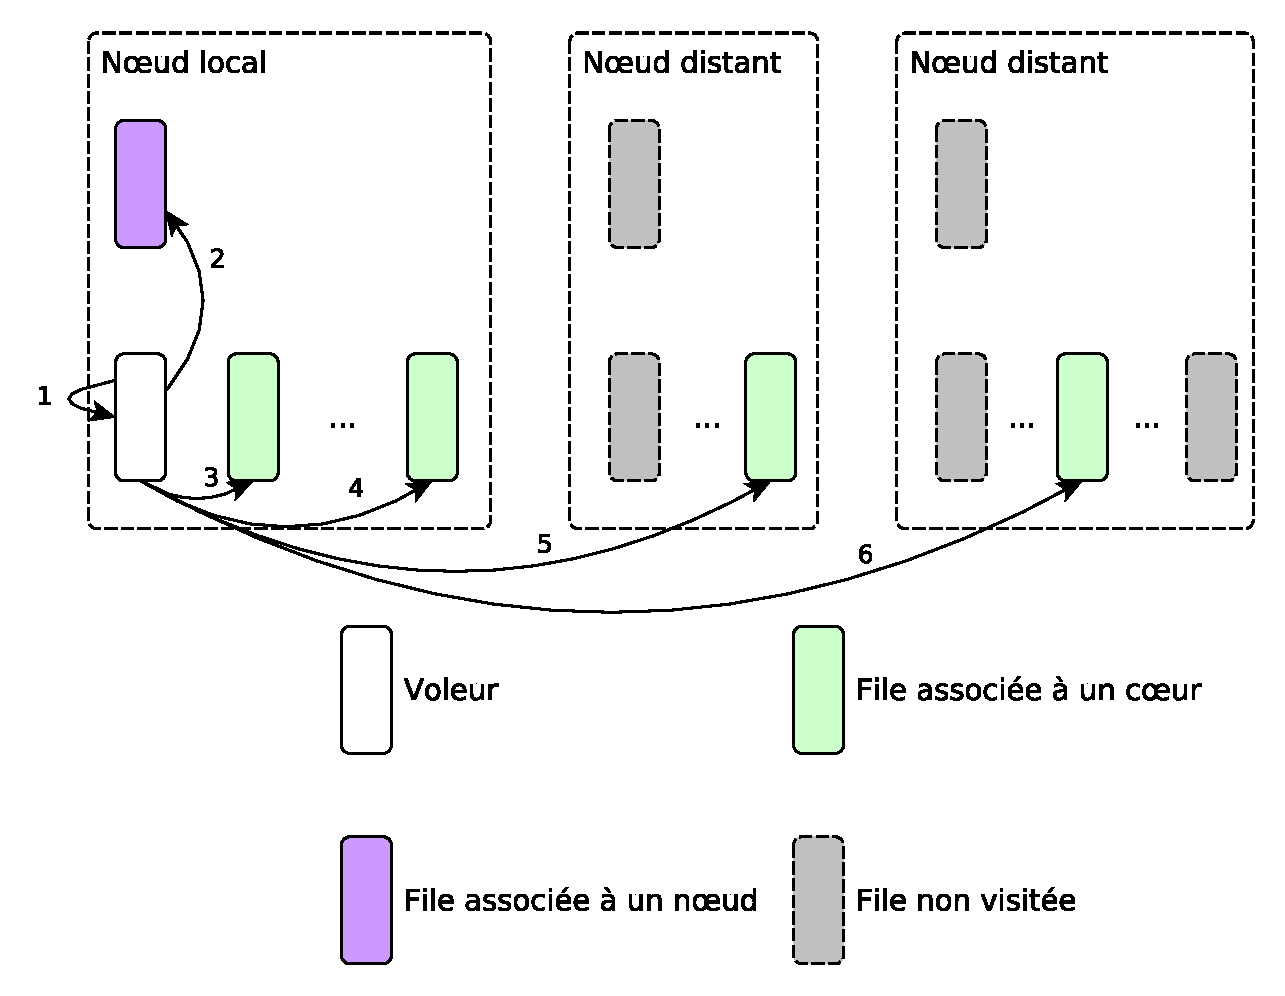
\includegraphics[width=0.73\textwidth]{steal_strategies_proc}
  \caption{Illustration de la stratégie \emph{sProc}, avec l'ordre de visite des files}\label{fig:openmp:runtime:steal_proc}
\end{figure}

\begin{figure}[h!]
  \centering
  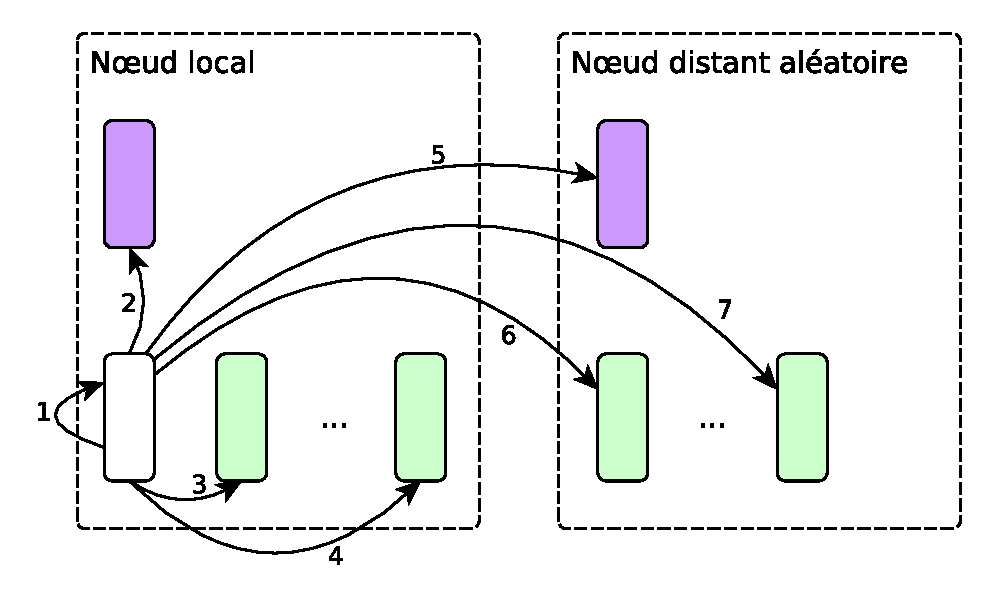
\includegraphics[width=0.6\textwidth]{steal_strategies_numa_proc}
  \caption{Illustration de la stratégie \emph{sNumaProc}, avec l'ordre de visite des files}\label{fig:openmp:runtime:steal_numa_proc}
\end{figure}

\begin{description}
  \item [sProc :] Cette stratégie est illustrée sur la figure~\ref{fig:openmp:runtime:steal_proc}. Le voleur va visiter sa propre file (1), celle de son nœud NUMA (2), puis va parcourir uniquement les files des cœurs en commençant par ses voisins (3, 4), puis en choisissant au hasard parmi les cœurs distant restant (5, 6).
  \item [sNuma :] Le voleur commence par visiter son nœud NUMA, puis les files des cœurs de son nœud, puis uniquement les files des nœuds NUMA distant.
  \item [sProcNuma :] Dans un premier temps le cœur voleur visite sa propre file. Si aucune tâche n'est disponible, il va ensuite visiter les files de tâches des cœurs voisins situés sur le même nœud.
    Si cela échoue de nouveau, il ira voler la file de son nœud NUMA.
    Si cela également, le reste de la topologie sera parcourue de manière similaire : un nœud sera choisi aléatoirement, les files des cœurs puis celle du nœud seront visitées.
  \item [sNumaProc :] Cette stratégie est illustrée sur la figure~\ref{fig:openmp:runtime:steal_numa_proc}~; elle est similaire à la précédente, mais l'ordre de parcours est inversé : après avoir visité sa propre file (1) le voleur regarde d'abord les files des nœuds NUMA (2) avant de regarder les files des cœurs (3, 4). De même que pour la stratégie précédente, le reste de la topologie est parcourue de manière similaire (5, 6, 7).
\end{description}


\subsection{Distribution des tâches d'initialisation}


La section~\ref{sec:openmp:langage:init} décrit comment un utilisateur peut avoir du contrôle sur la distribution des données de son application.
Cela passe par la distribution des tâches d'initialisation, et nécessite donc une modification du support exécutif.

Nous avons implémentés des stratégies additionnelles de placement des tâches prêtes, qui sont prioritaires sur toute autre stratégie décrite dans la section précédent, si une clause |init| est présente.
Elles correspondent directement aux stratégies décrites dans la section~\ref{sec:openmp:langage:init} : \textbf{random}, \textbf{cyclic}, \textbf{cyclicnuma}, et ont naturellement été implémentée en utilisant les files correspondantes de la hiérarchie.

\begin{todo}
  L'intérêt ici était de distinguer ce qu'on propose comme choix à l'utilisateur et comment c'est implémenté derrière.
  Mais bon ça fait un peu maigre comme section...
\end{todo}


\subsection*{Conclusion}

L'ensemble de ces modifications proposent un large choix de paramètres à ajuster pour le support exécutif, et ce n'est pas évident de voir a priori quelle(s) stratégie(s) devraient être privilégiée(s).

Y en a-t-il des meilleures que d'autres quelques soient les circonstances ?
Est-ce que que cela dépend du type d'application ? Du type d'architecture ?
La section suivante propose une évaluation détaillée de l'impact des différents points, et vise à dégager des conseils généraux vis à vis du choix des stratégies.


\section{Évaluation des extensions proposées}\label{sec:contribs:perf_eval}

Nous avons évalué les différentes améliorations proposées dans les sections~\ref{sec:openmp:langage} et~\ref{sec:openmp:runtime} sur les machines idchire et brunch, décrites en détails dans la section~\ref{sec:contribs:machines}.

La section suivante décrit les différents logiciels que nous avons utilisé pour nos expériences, ainsi que les modifications apportées le cas échéant ; et la section~\ref{sec:contribs:perf_eval:resultats} aborde point par point les extensions proposées.
Enfin la section~\ref{sec:contribs:perf_eval:libkomp} discute de l'application de nos idées dans un support exécutif différent, avec également une évaluation de performances.


\subsection{Logiciels}

Les logiciels utilisés pour nos expériences peuvent être divisé en trois catégories~:
\begin{itemize}
  \item Les applications utilisées
  \item Les supports exécutifs
  \item Les bibliothèques externes
\end{itemize}

Les applications et les supports exécutifs utilisées ont pu subire quelques modifications afin d'incorporer les modifications d'OpenMP proposées.
Ces changements sont décrits ci-dessous.
Nous n'avons effectué aucune modification aux bibliothèques externes, mais il est important de faire un point dessus, étant donné qu'une partie des performances peut en dépendre.

\subsubsection{Applications utilisées}

Les applications utilisées pour ces expériences proviennent des KASTORS\footnote{https://gitlab.inria.fr/openmp/kastors, branche 'affinity'}.

Nous avons ajouté une clause \emph{affinity} dans certaines applications~: dans le cas des applications d'algèbre linéaire, les tâches de calculs dépendent d'un ou plusieurs blocs de données. Nous avons ajouté une affinité entre chaque tâche et les données qu'elle écrit.
Dans le cas des applications de type stencil, nous avons ajouté une affinité vers un cœur précis pour les tâches successives.


\subsubsection{Supports exécutifs}


\paragraph{XKAAPI}~: nous avons implémentés les trois types d'extensions proposés dans la section~\ref{sec:openmp:runtime}, à savoir les différentes stratégies de distribution des données, les stratégies de sélection lors du vol de travail, et les stratégies de placement des tâches prêtes.
Ces modifications ont été rassemblées dans une version spécifique de XKAAPI~\footnote{https://scm.gforge.inria.fr/anonscm/git/kaapi/xkaapi.git, branche 'public/europar2016'}.


Nous avons pris comme base de comparaison les supports exécutifs fournis avec les compilateurs existant au moment de nos propositions.

\paragraph{GCC/libGOMP}~: nous avons utilisé la version 5.2.0 comme référence, sans y apporter de modification.

\paragraph{Clang/libOMP}~: nous avons utilisé la version 3.8. Bien que le support exécutif (libOMP) n'ait pas été modifié, le compilateur (Clang) a subit des modifications afin de supporter les clauses décrites dans la section~\ref{sec:openmp:langage}.

\subsubsection{Bibliothèques externes}

\paragraph{BLAS} : les applications d'algèbre linéaire des KASTORS dépendent de la bibliothèque BLAS.
Pour les expériences effectuées dans la section~\ref{sec:contribs:perf_eval:resultats}, nous avons utilisé la bibliothèque OpenBLAS~2.15 pour fournir les noyaux de calculs de base.


\paragraph{hwloc} : cette bibliothèque fournie les informations sur la hiérarchie de la machine, ainsi que des fonctions d'allocation de mémoire selon différentes politique (voir section~\ref{sec:context:os:lib}). Nous avons utilisé la version 1.11.0.

\paragraph{numactl} : nous avons utilisé \emph{numactl} pour certaines courbes de référence. \emph{numactl} est fourni par libNUMA ; nous avons utilisé la version par défaut fourni par le fabricant de la machine.


\subsection{Résultats}\label{sec:contribs:perf_eval:resultats}

\subsubsection{Impact de la distribution des données}

\begin{figure}[ht]
  \centering
  \includegraphics[width=\textwidth]{graph_distrib_data_idchire}
  \caption{Performances des différentes stratégies pour Cholesky en fonction de la distribution de données (N=32768, BS=512)}\label{fig:contribs:perf_eval:distrib-idchire}
\end{figure}

\subsubsection{Impact de l'affinité, et étude comparative des stratégies}

\begin{figure}[ht]
  \centering
  \includegraphics[width=\textwidth]{graph_all_strat_idchire}
  \caption{Performances des différentes stratégies pour Cholesky (N=32768, BS=512)}\label{fig:contribs:perf_eval:eval-strategies}
\end{figure}

\begin{figure}[ht]
  \centering
  \includegraphics[width=\textwidth]{graph_details_qr_cholesky_idchire}
  \caption{Comparaison de trois stratégies sur QR et Cholesky, en fonction de la taille de matrice}\label{fig:contribs:perf_eval:eval-qr-cholesky}
\end{figure}

\begin{todo}
GRAPHE : 5.5.2, Cholesky : (presque non-)impact stratégies affinité sur brunch/idkat
\end{todo}

\subsubsection{Affinité vers des cœurs}

\begin{figure}[ht]
  \centering
  \includegraphics[width=\textwidth]{jacobi_scale_iomp_komp}
  \caption{Performances de Jacobi en fonction de la version et du support exécutif}\label{fig:contribs:perf_eval:eval-jacobi}
\end{figure}

\subsection{Portage dans un autre support exécutif}\label{sec:contribs:perf_eval:libkomp}

\subsubsection{Description}

\subsubsection{Évaluation}

/!\ pour ces xp les versions de gcc/clang ont changé, ainsi que les BLAS !

\begin{todo}
  Il faut aussi comparer ça au simulateur. Peut être plus simplement faire une section à part.

  Vu que c'est principalement effectué avec le nouveau libkomp, peut être mettre ça dans une section suivant celle du "portage" vers le runtime intel.

  À discuter de où on met ça...
\end{todo}



\section{Dicussions et conclusion}


\begin{todo}

parler du fait qu'on pourrait avoir plus d'info, pour prendre de meilleures décisions

on pourrait tester de nouvelles heuristiques à travers un simulateur (ref chapitre 6)

\end{todo}







\part{Future work}

\begin{savequote}[6cm]
<< truc
\qauthor{Test}
\end{savequote}

\chapter{More OpenMP}\label{chap:contrib:TODO}
\chaptertoc

%\input{tex/future}
% This chapter should include:
% - What's left to do ?
% - Perspective

\begin{savequote}[6cm]
<< truc
\qauthor{Test}
\end{savequote}

\chapter{Conclusion}\label{chap:contrib:TODO}
\chaptertoc

%\part{Du concrêt}

C'est ici que j'écrit des trucs intéressant.

\begin{savequote}[6cm]
<< truc
\qauthor{Test}
\end{savequote}

\chapter{Some title dealing with runtimes}\label{chap:contrib:runtime}
\chaptertoc

%\lstset{language=PrologAstral}
\section{Conclusion}\label{sec:contrib:runtime:conclusion}

C'était cool



%\section{Conclusion}\label{sec:contrib:runtime:conclusion}

C'était cool

